\documentclass[12pt]{ucsddissertation}
% mathptmx is a Times Roman look-alike (don't use the times package)
% It isn't clear if Times is required. The OGS manual lists several
% "standard fonts" but never says they need to be used.
\usepackage{mathptmx}
\usepackage[NoDate]{currvita}
\usepackage{array}
\usepackage{tabularx}
\usepackage{booktabs}
\usepackage{ragged2e}
\usepackage{microtype}
\usepackage[breaklinks=true,pdfborder={0 0 0}]{hyperref}
\usepackage{graphicx}
\AtBeginDocument{%
	\settowidth\cvlabelwidth{\cvlabelfont 0000--0000}%
}
\usepackage{times}
%\usepackage[latin1]{inputenc}
\usepackage{fixltx2e}
\usepackage{xcolor}
\usepackage{footnote}
\usepackage{amssymb,amsfonts,amsmath}
\usepackage{booktabs}
\usepackage{graphicx}
\usepackage[export]{adjustbox}
\usepackage{subfig}
%\usepackage[sc]{mathpazo} % Palatino at 10pt is smaller than Times at 11pt
%\usepackage[scaled=0.86]{berasans}
\usepackage[scaled=1.03]{inconsolata} % Use Inconsolata instead of CMTT
\usepackage[T1]{fontenc}
\usepackage{pifont}
\usepackage{url}
\usepackage[htt]{hyphenat}
\usepackage{verbatim}
%\usepackage[explicit]{titlesec}
\usepackage[justification=centering]{caption}

%\usepackage[captionskip=5pt]{floatrow}
%\floatsetup[table]{style=plain}
%\setlength\textfloatsep{10pt}


\usepackage{color}
\usepackage{multirow}
%\usepackage{subcaption}
\usepackage{wasysym}
\usepackage{relsize}
\usepackage{array}
\usepackage{xspace}

% Clickable link colors here:
\definecolor{linkcol}{rgb}{0,0,0}
\definecolor{citecol}{rgb}{0,0,0}
\definecolor{urlcol}{rgb}{0,0,0.75}

\newcommand\xxx[1]{\textcolor{red}{\textbf{XXX: #1}}}

\newcommand\veryemph[1]{\textbf{#1}}

%\usepackage[bookmarks=true,%
%	bookmarksnumbered=true,%
%	colorlinks=true,%
%	linkcolor=linkcol,%
%	citecolor=citecol,%
%	urlcolor=urlcol,%
%	hypertexnames=true,%
%	pdfpagelabels]{hyperref}

%\usepackage[margin=1in]{geometry}


% Christian's magic space-saving stuff.
% http://www-h.eng.cam.ac.uk/help/tpl/textprocessing/squeeze.html
%

\renewcommand\floatpagefraction{.9}
\renewcommand\topfraction{.9}
\renewcommand\bottomfraction{.9}
\renewcommand\textfraction{.1}
\setlength{\parskip}{0em}
\frenchspacing

% Kirill's dainty list environments.

\newenvironment{prettylist}{
	\begin{list}{
		\footnotesize\raisebox{0.1mm}{\small\ding{118}}
	}{
		\setlength\topsep{2pt plus 1pt minus 1pt}
		\setlength\leftmargin{2em}
		\setlength\rightmargin{0pt}
		\setlength\itemsep{1pt plus.1pt}
		\setlength\parskip{0pt}
		\setlength\parsep{0pt}
		\setlength\itemindent{0pt}
	}
}{
	\end{list}
}

\newenvironment{catinfolist}{
	% Environment preamble
	\begin{list}{
		\% No label
	}{
		% List declaration
		%\raggedright
		\setlength\topsep{5pt plus 2pt minus 1pt}
		\setlength\leftmargin{12pt}
		\setlength\labelwidth{12pt}
		\setlength\rightmargin{0pt}
		\setlength\itemsep{1pt}
		\setlength\parskip{0pt}
		\setlength\parsep{0.25pt}
		\setlength\labelsep{0ex}
		\setlength\itemindent{0pt}
		\setlength\listparindent{0pt}
		\renewcommand\makelabel[1]{\bfseries$\circ$\hspace{6pt}\upshape ##1:\hspace{0.5em}}
	}
}{
	% Environment closing
	\end{list}
}

\newenvironment{categorylist}{
	% Environment preamble
	\begin{list}{
		\% No label
	}{
		% List declaration
		%\raggedright
		\setlength\topsep{5pt plus 2pt minus 1pt}
		\setlength\leftmargin{24pt}
		\setlength\labelwidth{12pt}
		\setlength\rightmargin{0pt}
		\setlength\itemsep{1pt}
		\setlength\parskip{0pt}
		\setlength\parsep{0.25pt}
		\setlength\labelsep{0ex}
		\setlength\itemindent{0pt}
		\setlength\listparindent{0pt}
		\renewcommand\makelabel[1]{\bfseries$\circ$\hspace{6pt}\upshape ##1:\hspace{0.5em}}
	}
}{
	% Environment closing
	\end{list}
}

\newenvironment{findinglist}{
	% Environment preamble
	\begin{list}{
		\footnotesize\raisebox{-0pt}{\footnotesize\ding{70}}
	}{
		\setlength\topsep{2pt plus 1pt minus 1pt}
		\setlength\leftmargin{2em}
		\setlength\rightmargin{0pt}
		\setlength\itemsep{1pt plus.1pt}
		\setlength\parskip{0pt}
		\setlength\parsep{0pt}
		\setlength\itemindent{0pt}
	}
}{
	% Environment closing
	\end{list}
}

\newenvironment{characteristics}{
	% Environment preamble
	\begin{list}{
		% No label
	}{
		% List declaration
		\setlength\topsep{5pt plus 2pt minus 1pt}
		\setlength\leftmargin{12pt}
		\setlength\labelwidth{0em}
		\setlength\rightmargin{30pt}
		\setlength\itemsep{1pt}
		\setlength\parskip{0pt}
		\setlength\parsep{0.25pt}
		\setlength\labelsep{0ex}
		\setlength\itemindent{0pt}
		\setlength\listparindent{0pt}
		\renewcommand\makelabel[1]{\bfseries\upshape ##1.\hspace{0.5em}}
	}
}{
	% Environment closing
	\end{list}
}

% Fine-tuning for table spacing. --cpk
\def\TblSpT{\rule[-1ex]{0pt}{0pt}}
\def\TblSpB{\rule{0pt}{2.5ex}}

% Column name formatting
\newcommand\colname[1]{\textit{#1}}

% Et al.
\newcommand\etal{\emph{et~al.}}

% Black filled circles with white number on it
% See Comprehensive LaTeX Symbol List --cpk
\def\blackI{\ding{182}}
\def\blackII{\ding{183}}
\def\blackIII{\ding{184}}
\def\blackIV{\ding{185}}
\def\blackV{\ding{186}}
\def\blackVI{\ding{187}}
\def\blackVII{\ding{188}}
\def\blackVIII{\ding{189}}

% Some kind of bibliography sorcery.

%\let\oldthebibliography=\thebibliography
%  \let\endoldthebibliography=\endthebibliography
%  \renewenvironment{thebibliography}[1]{%
%    \begin{oldthebibliography}{#1}%
%      \setlength{\parskip}{0ex}%
%      \setlength{\itemsep}{0ex}%
%  }%
%  {%
%    \end{oldthebibliography}%
%  }

% During paper preparation, "draft" should be set to true using the
% \drafttrue command in proposal.tex. For submission, set \draftfalse.

% For notes to authors. These are only enabled for draft versions. In
% non-draft versions \note does nothing.

\newcommand\noteby[2]{\note{#2\hspace{0.5em}---#1}}
\newcommand\notefor[2]{\note{\textbf{#1:} #2}}
\newcommand\pp[1]{\noteby{PP}{#1}}


%\titleformat\paragraph[runin]{}{}{1em}{\normalfont\normalsize\bfseries#1.}
%\titlespacing*\section{0pt}{1ex plus.5ex minus.2ex}{0ex plus .2ex}
%\titlespacing*\subsection{0pt}{1ex plus.5ex minus.2ex}{0ex plus .2ex}
%\titlespacing*\subsubsection{0pt}{1ex plus.5ex minus.2ex}{0ex plus .2ex}
%\titlespacing*\paragraph{0pt}{0.25ex plus.2ex minus.1ex}{0.5em}

\newcommand\emphpar[1]{\noindent\textbf{#1.}}
\newcommand\justpar[1]{\noindent\emph{#1.}}
\newcommand\finding{\noindent\ding{70}\hspace{0.5em}\textbf{Finding:}}
\newcommand\metrics{\noindent\ding{71}\hspace{0.5em}}
%%%
%%% PAPER-SPECIFIC MACROS
%%%

\newcommand{\eg}{{e.g.},\xspace}
\newcommand{\ie}{{i.e.},\xspace}
\newcommand{\et}{{et~al.}\xspace}

\def\ti{\textbf{\textsc{ti}}}
\newcolumntype{H}{>{\setbox0=\hbox\bgroup}c<{\egroup}@{}}

\newcommand\snapfeedsym{$\Circle$}
\newcommand\deltafeedsym{$\triangle$}
\newcommand\singlefeedsym{$\CIRCLE$}
\newcommand\aggfeedsym{$\LEFTcircle$}


\makeatletter

\renewcommand\paragraph[1]{%
\@startsection{paragraph}{4}{\z@}%
{-0.75ex plus 0.05ex}{-0.5em}%
{\normalfont\normalsize\bfseries}{#1}}

\renewcommand\section{%
\@startsection{section}{1}{\z@}%
{-1.25ex plus -0.5ex minus -.2ex}%
{0.75ex plus .25ex}%
{\reset@font\Large\bfseries}}

\renewcommand\subsection{%
\@startsection{subsection}{2}{\z@}%
{-1.25ex\@plus -0.5ex \@minus -.2ex}%
{0.5ex \@plus .2ex}%
{\reset@font\large\bfseries}}

\renewcommand\subsubsection{%
\@startsection{subsubsection}{3}{\z@}%
{-0.75ex\@plus -0.25ex \@minus -.25ex}%
{0.25ex \@plus .2ex}%
{\normalfont\normalsize\bfseries}}

\makeatother
\def\numallfeeds{XXX}
\def\numipfeeds{47}
\def\numhashfeeds{8}

% Scan feeds
\def\feedTSAlienVault{PA AlienVault IPs}
\def\feeddshield{DShield IPs}
\def\feedetiprep{Paid IP Reputation}
\def\feedpacketmail{Packetmail IPs}
\def\feedTSramnode{PA Packetmail ramnode}
\def\feedTSLabScan{PA Lab Scan}
\def\feedTSSnort{PA Snort BlockList}
\def\feedTSAnalyst{PA Analyst}


% Bot feeds
\def\feedTSCI{PA CI Army}
\def\feedTSBotscout{PA Botscout IPs}
\def\feedTSVoIP{PA VoIP Blacklist}
\def\feedTSCompr{PA Compromised IPs}
\def\feedTSBots{PA Blocklist Bots}
\def\feedTSHoneypot{PA Project Honeypot}


% Brute-force feeds
\def\feedbadipssh{Badips SSH}
\def\feedbadipbot{Badips Badbots}
\def\feedTSBrute{PA Brute-Force}
\def\feedusername{Badips Username Notfound}
\def\feeddisco{Haley SSH}
\def\feednothink{Nothink SSH}
\def\feeddangerrule{Dangerrulez Brute}
\def\feedTSScopVoIP{PA ScopServ VoIPBL}


% Malwre feeds
\def\feedfeodo{Feodo IP Blacklist}
\def\feedTSLabMalware{PA Lab Malware}
\def\feedmalcode{Malc0de IP Blacklist}
\def\feedTSBambenek{PA Bambenek C2 IPs}
\def\feedTSSSL{PA SSL Malware IPs}
\def\feedTSAbusech{PA Abuse.ch Ransomware}
\def\feedTSMalTraffic{PA Mal-Traffic-Anal}
\def\feedzeus{Zeus IP Blacklist}

% Exploit feeds
\def\feedbadiphttp{Badips HTTP}
\def\feedbadipftp{Badips FTP}
\def\feedbadiprfi{Badips RFI}
\def\feedbadipdns{Badips DNS}
\def\feedbadipsql{Badips SQL}

% Spam feeds
\def\feedbadippostfix{Badips Postfix}
\def\feedbadipspam{Badips Spam}


\def\feedFBBasecamp{FB Aggregator$_1$}
\def\feedFBZendesk{FB Aggregator$_2$}
\def\feedFBAdmin{FB Malicious IPs}

\def\feedalienvault{Alienvault IP Reputation}


% Malware md5 hash feed.
\def\feedTSOSINT{PA OSINT}
\def\feedTSmalcode{PA Malc0de}
\def\feedTSMobile{PA Mobile Malware}
\def\feedTSRAT{PA RAT Hunter}
\def\feedTSBackdoor{PA Backdoor \& RAT}




% Definition of feed name
\def\spamhausdrop{Spamhaus DROP}
\def\spamhausedrop{Spamhaus EDROP}
\def\dshieldtop{DShield Top Blacklist}
\def\ciarmy{CI Army Blacklist}
\def\etcompromised{ET Compromised}
\def\snortfilter{Snort IP Filter List}
\def\bdsatif{BDS IP Ban List}
\def\feodo{Feodo IP Blacklist}
\def\ettor{Tor IP Blacklist}
\def\blocklistde{Blocklist De Blacklist}


% Definition of reflector
\def\reflector{reflector}
\def\Reflector{Reflector}
% Definition of reflector plural
\def\reflectors{reflectors}
\def\Reflectors{Reflectors}
% Definition of reflector capitalized
\def\reflectorcap{Reflector}

% Definition of reflector count
\def\reflcount{222,782}

% Definition of reflector rough number
\def\reflroughnum{220K}

% Definition of blacklist number
\def\blacklistnum{9}

% OGS recommends increasing the margins slightly.
\increasemargins{.1in}

% These are just for testing/examples, delete them
\usepackage{trace}
%\usepackage{showframe} % This package was just to see page margins
\usepackage[english]{babel}
\usepackage{blindtext}
\overfullrule5pt
% ---

% Required information
\title{An Empirical Analysis on Threat Intelligence: Data Characteristic and Real-World Uses}
\author{Guo Li}
\degree{Computer Science}{Doctor of Philosophy}

\cochair{Professor Kirill Levchenko}
\cochair{Professor Stefan Savage}
% Your committee members (other than the chairs) must be 
% in alphabetical order
\committee{Professor Deian Stefan}
\committee{Professor Geoffrey M. Voelker}
\committee{Professor Xinyu Zhang}
\degreeyear{2020}

% Start the document
\begin{document}
% Begin with frontmatter and so forth
\frontmatter
\maketitle
\makecopyright
\makesignature


% Optional
\begin{dedication}
\setsinglespacing
\raggedright % It would be better to use \RaggedRight from ragged2e
\parindent0pt\parskip\baselineskip
\centering
To everyone who has supported me.
\end{dedication}


% Optional
%\begin{epigraph}
%\vskip0pt plus.5fil
%\setsinglespacing
%\vfil
%\begin{center}
%``The cowards never started, and the weak died along the way.
%That leaves us.''
%\vskip\baselineskip
%\textit{Phil Knight}
%\end{center}
%\vfil
%\end{epigraph}



% Next comes the table of contents, list of figures, list of tables,
% etc. If you have code listings, you can use \listoflistings (or
% \lstlistoflistings) to have it be produced here as well. Same with
% \listofalgorithms.
\tableofcontents
\listoffigures
\listoftables



% Preface
%\begin{preface}
%Almost nothing is said in the manual about the preface. There is no
%indication about how it is to be typeset. Given that, one is forced to
%simply typeset it and hope it is accepted. It is, however, optional
%and may be omitted.
%\end{preface}


% Your fancy acks here. Keep in mind you need to ack each paper you
% use. See the examples here. In addition, each chapter ack needs to
% be repeated at the end of the relevant chapter.
\begin{acknowledgements}
First and foremost, I would like to thank my advisors, professor Stefan
Savage and professor Kirill Levchenko. When I first joined the PhD program,
I was an introvert student with little understanding of research. I was
too scared to try something new or to think boldly. Thanks to my advisors,
who both have very clean visions and are not afraid to take risks, I had a 
very wild PhD experience. We tried a completely new idea for malware 
analysis, reverse-engineered Volkswagen engine firmware to try to disclose 
its cheating logic, and eventually moved to Threat Intelligence and try to 
picture the landscape of threat on the Internet. Some projects worked out, 
some did not, but I learned so much from this journey. They taught me
to always follow my interests, not the trend, and never be afraid of 
failure. This attitude towards research had changed me a lot, both in the
way of doing research, also in the way of making life decisions. Besides, 
I really appreciate that both of my advisors gave me great freedom during
my study, which makes my PhD journey a lot less stressful, and at the same 
time taught me to be independent very early on.

I also liked to thank professor Geoffrey M. Voelker. Although he is not my
official advisor, he helped me a lot during two of my projects, both of 
which are covered in this dissertation. He also gave me a lot of valuable 
guidance during some of my lowest points. I really thank his kindness
and caring. I would also like to thank Professors Deian Stefan and Xinyu Zhang 
for being on my doctoral committee and being available whenever I needed help.

PhD experience is fun but also challenging, and I can not make it 
without the help from so many people, especially from my ``Foundry'' lab
mates (CSE 3142), where everyone is so kind and supportive.
Our lab has a very free, open atmosphere, and we discuss almost anything
freely here. With these discussions and exchange of ideas, I become 
more objective on thinking, and learned a lot on many different 
topics. We are also hard-working and spent many long nights together
at lab. I will never forget those times when we laugh and fight together. 
I would also like to thank members from ``Tiger'' lab (CSE 3152), we 
hang out frequently and give support to each other during hard times. The style 
of how they approach research problems---being very strict on defining the
problem and validating with real-world examples---inspired me a lot.

Special thanks to Danny Huang and Tianyin Xu. These two senior students(now 
both become professors) had helped me a lot during my PhD and give me
valuable advice. During my lowest points, I had multiple long conversations
with them, and they shared a lot of their own stories and encouraged me to
keep going. Their encouragement and the experience they shared is critical 
for my journey.

I would like than all the member of Sysnet group, including all the faculties,
staffs and students. It has been a wonderful 6 years for me, and I had many 
interactions with many people during this process, in security lunch, 
syslunch, sysnet hiking, CNS meeting etc. All these activities not only enable
me to learn a lot of stuff, but also make my journey much more enjoyable, and 
give me a strong feeling of belonging. Special thanks to Cindy Moore, who 
helped me numerous times setting up servers and fixing network issues. 

Chapter~\ref{chapter:data_character}, in part, is a reprint of the material 
as it appears in Proceedings of the Usenix Security 2019. \textit{Reading the 
Tea Leaves: A Comparative Analysis of Threat Intelligence.} Vector Guo Li,
Matthew Dunn, Paul Pearce, Damon McCoy, Geoffrey M. Voelker, Stefan Savage,
Kirill Levchenko. The dissertation author was the primary investigator and 
author of this paper. I really like to thank my coauthors on this paper,
without who I will never be able to finish this work. I like to especially 
thank Paul Pearce, who helped me a lot throughout the project. At the
beginning, when I had little idea about what to do and was so unfamiliar with 
data analysis tools, he gave me critical hands-on assists. I am also very
grateful to Alberto Dainotti and Alistair King for sharing the UCSD telescope
data and helping me with the analysis, also professor Micheal Bailey for 
sharing the Mirai Botnet data. Besides, I like to thanks professor Aaron 
Schulman, who encouraged me a lot when the first submission of this paper 
was rejected, and helped me regain my confidence in the work.

Chapter~\ref{chapter:data_usage}, in part, is a reprint of the material as 
submitted to the Proceedings of the Usenix Security 2020. \textit{
Clairvoyance: Inferring Blacklist Use on the Internet} Vector Guo Li, 
Gautam Akiwate, Yihui Chen, Geoffrey M. Voelker, Kirill Levchenko, Stefan 
Savage. The dissertation author was the primary investigator and author of 
this paper. I really appreciate the help from my coauthors, especially 
Gautam Akiwate. He helped me a lot on data collection and analysis,
and I really learned a lot from the way he looks at data problems. 
Furthermore, he gave me crucial moral support during some critical times
of the project. I will not be able to finish this work without his help.
I also really appreciate the suggestions I received from kc Claffy and 
Alex Gantman regarding this project.

Last but not least, I want to thank my parents. My parents know little
about research, but they know how to do things. They gave me lots of 
suggestions on my study, but I was too fool to realize how valuable those 
suggestions are. This journey is tough, and many times when I did not
know what to do, when I lost my hope, when I thought about giving up,
they supported me, encouraged me, gave me strength and hope to 
carry on and keep going. If the PhD journey is walking through a dark 
tunnel, then they are the torch in my hand that are always there,
calm me down, show me the way and bring me warmth. They are the source of 
my strength and my motivation to work hard. It is very lucky for me to have 
such wise and supportive parents, and I will never forget their love 
and caring.
\end{acknowledgements}


% Stupid vita goes next
\begin{vita}
\noindent
\begin{cv}{}
\begin{cvlist}{}
\item[2014] Bachelor of Science, Peking University
\item[2014--2020] Research Assistant, University of California, San Diego
\item[2017] Master of Science in Computer Science, University of California, San Diego
\item[2020] Doctor of Philosophy in Computer Science, University of California, San Diego
\end{cvlist}
\end{cv}
\end{vita}


% Put your maximum 350 word abstract here.
\begin{dissertationabstract}

Threat Intelligence, both as a concept and a product, has been increasingly
gaining prominence in the security industry. At a high-level, it is the 
``knowledge'' that helps organizations understand and mitigate cyber-attacks.
Most commonly, it refers to the collection of threat indicators---IP 
addresses, domain names, file hashes, etc. known to be associated with 
attacks. By compiling and distributing this information, it is believed 
that recipients will be able to better 
defend their systems from future attacks. Thus, there are now hundreds of
vendors offering their threat intelligence solutions as a mix of public and
commercial products. 

However, our understanding of this data, its characterization, and the
extent to which it can meaningfully support its intended uses, is
still quite limited. Furthermore, how the data is being used by
organizations, how popular it is, and what impact it could have on the 
Internet are also not clear to our community. We lack an empirical 
assessment of real-world threat intelligence, both in terms of the data
itself and its usage, and it is important to first understand the current 
status of threat intelligence, then can we reasonably discuss how to make
improvements.

In this dissertation, I take an empirical approach to study threat 
intelligence and try to address these gaps. In particular, I explore 
this topic from two perspectives: 1) the characteristic and dynamics of 
threat intelligence data feeds and 2) how they are used in the 
real-world. In particular, I formally defined a set of metrics for 
analyzing threat intelligence data feeds and use these measures to 
systematically characterize a broad range of public and commercial feeds. 
Further, I ground my quantitative assessments using external measurements 
to qualitatively investigate issues of coverage and accuracy. Finally, I
designed a method using the IP ID side channel to test if a remote host 
is blocking traffic from a given IP address. Using this technique, I 
measure over {\reflroughnum} U.S. hosts and test whether they 
consistently block connections with IPs identified on popular IP blacklists. 
Beyond these blacklists, I also demonstrate the evidence for more widespread 
use of other blacklists for traffic blocking. Together, my work provides
an in-depth look into the current picture of threat intelligence and augments
the knowledge of our community on this topic.

\end{dissertationabstract}


% This is where the main body of your dissertation goes!
\mainmatter

% Optional Introduction
% Optional Introduction
\chapter{Introduction}

Computer security is an inherently adversarial discipline in which
each ``side'' seeks to exploit the assumptions and limitations of the
other.  Attackers rely on exploiting knowledge of vulnerabilities,
configuration errors or operational lapses in order to penetrate
targeted systems, while defenders in turn seek to improve their
resistance to such attacks by better understanding the nature of
contemporary threats and the technical fingerprints left by attacker's
craft.  Invariably, this means that attackers are driven to innovate
and diversify while defenders, in response, must continually monitor
for such changes and update their operational security practices
accordingly.  This dynamic is present in virtually every aspect of the
operational security landscape, from anti-virus signatures to the
configuration of firewalls and intrusion detection systems to incident
response and triage.  Common to all such reifications, however, is the
process of monitoring for new data on attacker behavior and using that
data to update defenses and security practices. Indeed, the extent to
which a defender is able to gather and analyze such data effectively
defines a de facto window of vulnerability---the time during which an
organization is less effective in addressing attacks due to ignorance
of current attacker behaviors.

This abstract problem has given rise to a concrete demand for
contemporary threat data sources that are frequently collectively
referred to as \emph{threat intelligence}. Threat Intelligence 
is the \emph{knowledge} that allows organizations to understand and 
mitigate cyber-attacks. This ``knowledge'' involves a wide variety 
of things. It can be vulnerability reports, where system and 
network administrators can learn the vulnerabilities and the potential
impact on their systems. It can also be IP or domain blacklists,
which tell users where the attacks are originating from, so people
can take precautions against these indicators. It can even be some 
online discussion thread in an underground forum, so security 
experts can track what malicious actors are discussing about. 
All of these knowledge can help security experts better understand 
potential threats, and then better help organizations to defend 
against them.

By far the most common form of Threat Intelligence are so-called 
\emph{indicators of compromise:} simple observable behaviors that 
signal that a host or network may be compromised. These indicators 
are in general straightforward forensic data that are directly 
associated with attacks. The most notable examples are:
\begin{prettylist}
    \item \textbf{IP Addresses}: IPs known to launch particular 
    attacks, like port scanning, brute-force login, etc.
    \item \textbf{Domain Addresses}: Domains known to host 
    Command-and-Control servers or sending spam emails, etc.
    \item \textbf{URLs}: Compromised websites or phish URLs, etc.
    \item \textbf{File Hashes}: Indicating a file or executable 
    known to be associated with a particular variety of malware, etc.
\end{prettylist}

The presence of such indicators in a system or network is a symptom 
that alerts an organization to a problem. For example, if one 
machine in an organization contacted a domain that known to be
associated with malware Command-and-Control servers, it is a strong
indication that this machine is probably infected with the 
corresponding malware. Part of an organization's defenses 
should reasonably include monitoring its assets
for such indicators to detect and mitigate potential compromises as
they occur. And these indicators are simple enough that they can be
easily integrated into defense or monitoring systems, like network
firewalls or malware scanners.

While each organization naturally collects a certain amount of threat
intelligence data on its own (e.g., the attacks they repel, the e-mail
spam they filter, etc.). any single entity has a limited footprint and
few are instrumented to carefully segregate crisp signals of attacks
from the range of ambiguity found in normal production network and
system logs. Thus, it is now commonly accepted that threat
intelligence data procurement is a specialized activity whereby
third-party firms, and/or collections of public groups, employ a range
of monitoring techniques to aggregate, filter and curate quality
information about current threats.  Indeed, the promised operational
value of threat intelligence has created a thriving (multi-billion
dollar) market~\cite{timarket}. 

Most established security firms, like Cisco Security~\cite{ciscotalos}, 
Palo Alto Networks~\cite{panautofocus}, Fortinet~\cite{fortinet} etc, 
and many specialized companies, like CrowdStrike~\cite{crowdstrike}, 
Anomali ThreatStream~\cite{anomali}, Recorded Future~\cite{recordedfuture}
etc,. are all offering threat intelligence solutions. Public threat
intelligence providers like Spamhaus, Abuse.ch, Dshield etc, are also 
getting more and more attentions. The global threat intelligence market is
predicated to surpass \$13 Billion in 2025~\cite{tipredict2018}. With the
industry thriving, there is also a rapid increase in the related research
works~\cite{tounsi2018survey}, covering topics from data characteristic,
effectiveness evaluation to design better sharing systems and protocols.

From a high level, there are two major aspects of Threat Intelligence: 
\textit{Data} and \textit{Operation}. \textit{Data} represents the content 
of Threat Intelligence---the actual information provided in different Threat
Intelligence products. \textit{Operation} represents the usage of 
data---different ways people can use Threat Intelligence to help. This
generalization is common for all data-based products. Therefore,
all research problems related to Threat Intelligence can be categorized into
these two areas: analyzing threat intelligence data itself, or exploring
ways to use the data.

When looking at these two general problems, one can further 
take two different research approaches: \textit{Empirical} and 
\textit{Algorithmic}. \textit{Empirical} approach focuses on understanding
the current ecosystem of Threat Intelligence, including studying the 
data characteristic, measuring different use cases, discover potential 
shortcomings, etc. This approach emphasizes on thoroughly understanding
existing solutions, uncovering patterns and underlying logic, 
so the community can gain valuable insights.
\textit{Algorithmic} approach, on the other hand, 
focuses on designing new algorithms to 
improve current solutions, like new threat hunting algorithms to improve 
Threat Intelligence data quality, or better ways to utilize these data 
during operation, etc. This approach emphasizes on designing new solutions 
to improve existing ones, so the community can have better algorithms and
tools to work with Threat Intelligence.

\begin{figure}
\centering
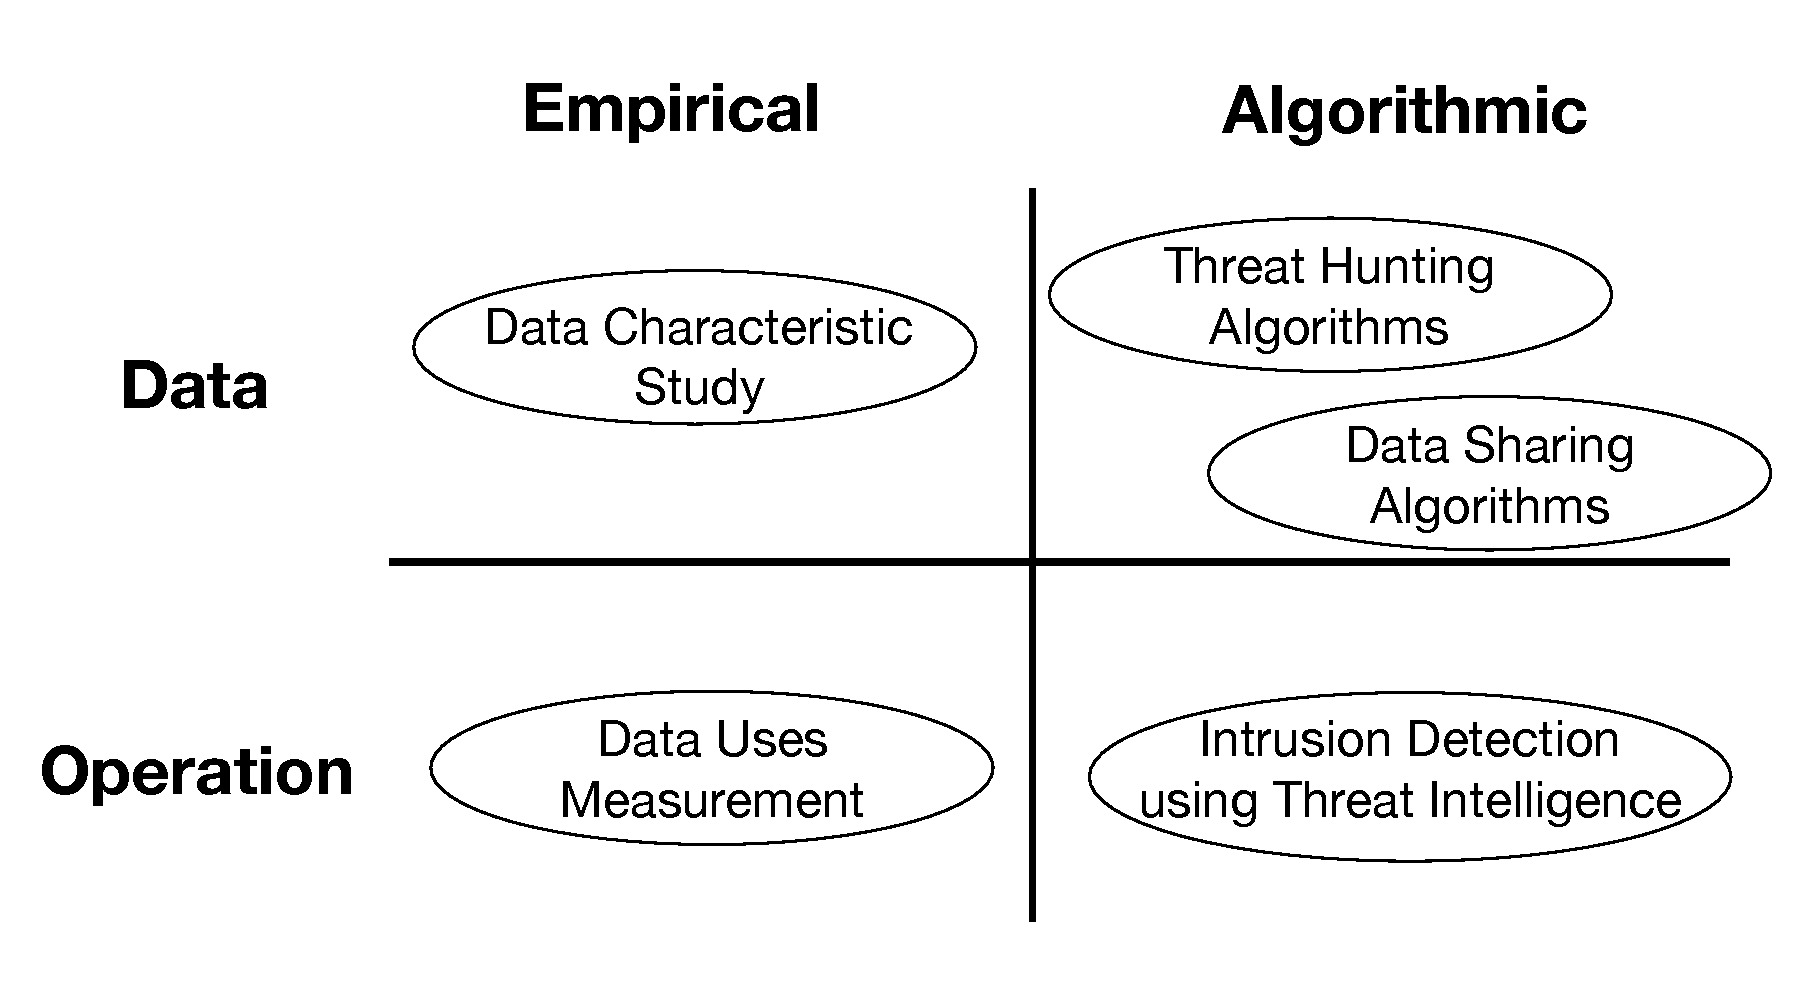
\includegraphics[width=0.8\textwidth]{threat_intel_research_overview.pdf}
\caption{Threat Intelligence research overview and example research
topics in each direction.}
\label{fig:threat_intel_overview}
\end{figure}

Therefore, research directions related to Threat Intelligence can be 
viewed in four general categories, as illustrated in
Figure~\ref{fig:threat_intel_overview}. More specifically, the four 
research directions are: 
\begin{prettylist}
    \item Empirical analysis on Threat Intelligence data: \\
    Understanding the characteristic of Threat Intelligence data, different
    data generation systems and their performance, different threat sharing
    strategies and how are they being used in the real-world, etc.
    
    \item Algorithm exploration related to Threat Intelligence data: \\
    Designing algorithms for threat hunting (Threat Intelligence generation),
    specification for data description and protocols for data sharing, etc.
    
    \item Empirical analysis on Threat Intelligence usage: \\
    Measuring how organizations are using Threat Intelligence, the problems 
    when using these data and the impact on the Internet, etc.
    
    \item Algorithm exploration related to Threat Intelligence usages: \\
    Designing better methods to use threat intelligence during system and 
    network defense(e.g. increasing coverage, reducing false positives),
    explore new ways to use threat intelligence data, such as using the 
    data as machine learning training data, etc.
\end{prettylist}

In this dissertation, I take an empirical approach and explore the 
\textit{Data} and \textit{Operation} problems of Threat Intelligence.
I focus on thoroughly understanding the current status of Threat 
Intelligence and will then discuss my takeaways from these analyses.
In the study of \textit{Data}, which will be discussed in Chapter~\ref{chapter:data_character}, 
I analyzed the data characteristics of existing Threat Intelligence products.
I designed mathematics metrics for Threat Intelligence data evaluation,
and with these metrics, I studied \numipfeeds\ distinct IP address 
data feeds, covering six categories of threats, and \numhashfeeds\ distinct
malware file hash feeds, and measured their data characteristic. Through this
work, I revealed the limitation of existing Threat Intelligence data and 
discussed the potential improvements based on my findings. In the study of
\textit{Operation}, which will be discussed in Chapter~\ref{chapter:data_usage},
I measured how Threat Intelligence data is being used on a large scale. 
I designed a method using IP ID side channel that can measure the 
connectivity between two Internet hosts from a third point. With this 
method, I conducted a large scale Internet measurement over {\reflroughnum} 
U.S. hosts and uncovered their uses of {\blacklistnum} popular public IP
blacklists. I further investigated a broader use of blacklists among the 
hosts, and discovered over 73K hosts has shown blacklist related blocking 
behavior. Together, my work provided an in-depth look into the current
status of Threat Intelligence and augmented the knowledge of our community
on this topic.

%\verb!\mainmatter! macro because it should start on page~1.
%\end{dissertationintroduction}

\chapter{Background}
\label{chapter:background}

\section{Threat Hunting}
\subsection{Intrusion Detection}

One direct way to capture threat is to identify the attacker when a
system in use is under attack, so we can capture the 
attacker in action. These systems can be specially deployed systems
just for luring attackers, like honeypot; they can also be real systems
with real users, where people deploy detection system and capture 
attacks when they are happening. The technique we use here is also 
the technique to protect the system in the first place:
\textit{Intrusion Detection}.

Intrusion detection aims to detect attacks on network or system on the
fly. The techniques involved can generally be classified as two 
categories: misuse-based detection and anomaly-based detection.
Misuse-based approaches utilize pre-defined patterns and signatures
of malicious behaviors, and dynamically compare the behavior of the
system against these patterns to spot potential intrusion. On the another
hand, anomaly-based detection construct a model for the normal behavior 
of a system, then check if the current behavior is deviating from the 
``normal'' behavior.

The performance of misuse-based detection methods depends on the quality
of the pre-defined attack patterns (or detect policies), and these 
patterns are usually provided manually by security experts. Since 
different attack vectors vary a lot on their approaches and system 
component they touch, the 
patterns provided by the detection system must be able to cover a 
diverse set of behavior, also to be extendable, as new attacking
methods are keep showing up. Therefore, early work on this technique like
Bro~\cite{paxson1999bro}, Snort~\cite{roesch1999snort}, 
P-BEST~\cite{lindqvist1999detecting}, and STAT~\cite{vigna2003designing}
all emphasize on the providing a powerful threat modeling language, which
can express a broad set of threat, also easy to program to include new 
patterns. Recent works like~\cite{bugiel2012towards} move to new
system environment (e.g. mobile system like Android), but still focus
on providing a expressive modeling language to build detect policies. 
These misuse-based detection methods is generally accurate, since the
pre-defined attack patterns are usually well defined by security experts. 
The main disadvantage of this technique is that it can only detect 
modeled attacks. For new type of attacks where there are no pattern
written, misuse-based system will miss them completely.

As a complementary, anomaly-based detection methods try to detect if
the behavior of an application or system is different from its benign
behaviors. This technique relies on modeling the normal behavior of a 
system in question, and since there are so many possible things a program 
can do, we need to simplify the ``behavior'' to precisely reason about 
it. Forrest et. al.~\cite{forrest1996sense} first proposed to use
syscall sequence of a program as its behavior, since a program can only
affect the operating system with syscalls, and from the security 
perspective, these would be the only behaviors that matters. Follow up
works like ~\cite{lee1998data, warrender1999detecting, mutz2006anomalous}
explored different data model to better distinguish abnormal sequences
from benign ones, using method like data mining, Bayesian network and 
neural network. Recent works like~\cite{du2017deeplog} also try to 
utilize more data sources and experiment with more advanced machine
learning algorithm for the detection. The advantage of these approaches 
is that it can capture previously unknown attacks. However, it tends
to suffer more false positives, since a normal program can show abnormal
behaviors once a long while, and it is very hard to capture these
cases when we first build the ``normal'' behavior set for a program.

\subsection{Causality Analysis}
Intrusion detection techniques described before detects threats 
when abnormal behavior is observed. But for many advanced 
attacks, especially the APTs(Advanced Persistent Threats), it 
is not always obvious to trace from the malicious behavior, e.g.
a running malware, to the source of the attacks, e.g. a phish 
URL that distributes the malware. This is mainly because sophisticated
attacks often take precautions to hide their traces by deleting
system or application logs, they can also prolong the attacks, 
creating a large window from the time they break into victims' 
machines till the time they actually carry out malicious activities. 
All of these can create difficulties for administrators to diagnose
the intrusion and trace the source. In the context of Threat 
Intelligence, it is important to uncover the source of 
an attack, so we can provide valuable indicator-of-compromise for the 
community to defense the same attack in an early stage.

The analysis, which tracks causal relationships between files and 
processes to diagnose attack provenances and consequences, is called
\textit{Attack Causality Analysis}. It is an critical technique
during threat intelligence hunting. The pioneering work in this field
is done by King and Chen~\cite{king2003backtracking}. They first defined
the event dependency graph, where the nodes represent processes and files
and edges represent the events between process and files, for example,
a process spawn another process, or a process read or write to a 
file. Given a detection point, like a suspicious files or a running
process, the system builds a dependency graph from this points by
processing event logs, then using the timestamp of each events and 
their causal relationship, we can trace back to the source and identify
the original intrusion point.

A simple idea as it seems, it captured the fundamental logic behind 
causality analysis: information flow tracking. However, this simple
solution quickly runs into a problem in a complex system: 
\textit{dependence explosion}~\cite{goel2005taser}, where there are 
so many processes and files involved in this dependency graph, together
with large amount inter-relations, that it is very hard identify the
real attack from the haystack. The case become even more true when there
are long-running programs, like a server program. The dependency 
associated with these program will grow enormously over 
time~\cite{lee2013high}, making the dependency graph even more 
complicated.

Many work have tried to tackle this problem. Some heuristics have been 
proposed to prune the graph, like in~\cite{king2005enriching}, the 
authors utilized the fact that worms try to exploit from host to host,
so the traffic from a host who already has an IDS alert is more likely
associated with worm attacks. Liu et al.~\cite{liu2018towards} uses
the rareness of events as a metric to prioritize searching on dependency
graphs. Other work try to break the entities on the graph into smaller 
granularity, so we can pinpoint the causal relationship between objects.
For example, Goel et al.~\cite{goel2005taser} use the separate socket
reads to partition the execution of a program into different segments, 
so the monitoring system can figure out which action of that program
is corresponded with which exact network request. Lee et 
al.~\cite{lee2013high} use the prevalence of event-loops in programs to
partition the execution of the program based on each loop iteration,
and then associates events with specific loop iterations. Binary taint
tracking has also been utilize to provide richer semantic information, 
like demonstrated in~\cite{ma2016protracer}. This topic is still an 
active topic today and researcher are trying to solve this from different
angle.
\subsection{Malware Analysis}
Malicious software, often called malware, is always a pressing threat 
on the Internet. It has been used by attackers to steal sensitive user data, 
control victim machines to launch spam campaigns or DDoS campaigns, or 
encrypt valuable data to demand ransom, etc. Symantec has reported over 200 
Million new malware variants just in 2018 alone~\cite{symantecmalware}. 
Therefore, it is crucial for threat intelligence products to cover recent 
malware comprehensively.
Malware threat intelligence data usually comes as two forms: file hashes,
like MD5, that represent malware variants themselves, and IPs or domains
that host Command-and-Control servers for the malware. Both forms of 
data is critical for organizations, as the presence of either form 
indicates a strong possibility of compromise, and immediate actions need 
to be taken. To generate these data, security companies rely on analyzing 
unknown binaries, collected from the Internet or uploaded by customers,
to determine if they are malicious.

To identify if an unknown binary is malware, one straightforward yet
effective way is to check if the binary is a variant of known malware.
Since it is nontrivial to develop a sophisticated malware program, 
attackers tend to just modify existing malware to generate new unseen
variants. Some typical ways include code transformation(e.g. replace ``mov 
eax, 0'' with ``xor eax, eax''), obfuscation, or encrypting the original 
binary and stores the result as data in a new executable (with a packer 
program). These simple techniques enable attackers to quickly generate a 
large number of variants from a single malware instance, and significantly 
increase the overhead for security experts to analyze them.

To compare a new malware sample with existing ones, we need to define a 
suitable representation of malware samples, from which we can calculate 
the similarity between them. There are two approaches to construct this 
``representation'': \textit{Content-based} and \textit{Behavior-based}. 
Content-based approach abstracts a program based on its code content, and 
calculate the similarity between programs by comparing their code. 
Early work by M. Gheorghescu~\cite{Gheorghescu2006ANAV} propose 
to break the malware program into basic blocks and compare the similarity 
between those blocks.
Dullien et al.~\cite{dullien2005graph} extract control flow graphs from 
malware programs and use graph similarity as the similarity between programs.
These content-based approaches rely on analyzing program code itself, so 
they still suffer the problem of advanced code obfuscation, which can modify
the code dramatically while maintaining the same functionality. This leads to
the behavior-
based approach, where we extract the actual behavior of malware and use that
as the signature for comparison. Lee et al.~\cite{lee2006behavioral} propose
to use system call sequence as the signature to classify different malware
samples. Bailey et al.~\cite{bailey2007automated} use the \textit{non-transient
state changes} malware causes on a system(files written, processes created) as 
the behavior signature, and do the comparison based on these behaviors. Holz 
et al.~\cite{rieck2008learning} further developed this behavior-based method, 
and use the actions of malware as machine learning features, and use a 
supervised machine learning model to conduct the comparison and classification.
Bayer at al.~\cite{bayer2009scalable} used taint tracking to capture a finer
granularity of malware's behavior, and use this information for more precise
identification. The behavior-based approaches usually capture the behavior of
malware through dynamically executing the malware samples, so it won't be 
affected by malware code itself, but executing the code for every variant in
question impose nontrivial overhead. 

When there is no existing malware to compare with, or the program in question 
does not match any known malware, an analysis system will need to decide if
the program is malicious just based on the behavior of the program itself. Like
the intrusion detection methods described in the previous section, the logic
here also relies on having ``specifications'' that cover potential malware 
behaviors, and check if the analyzed program exhibits those behaviors. One 
common heuristic is to check if the program makes any changes to the system
registry. GateKeeper~\cite{wang2004gatekeeper}, for example, detect spyware
by monitoring if the program register as an OS auto-start extension, such as 
an NT service, a tray icon in Windows, or a Unix daemon/cron job. Other tools
also check different detection points, like VICE~\cite{bulter2004vice}, which
checks for the existence of various hooks used by rootkits. More advanced 
systems tend to further monitor the detailed behavior of the program, like 
in~\cite{kirda2006behavior}, the authors try to detect a popular type of
spyware that uses Internet Explorer’s Browser Helper Object (BHO) and 
toolbar interfaces to monitor a user’s browsing behavior. The system uses 
dynamic analysis to track if the program monitors users' actions and sends
out its findings to an external entity. Panorama~\cite{yin2007panorama}, 
similarly, use dynamic taint tracking to construct the information flow of
an unknown program, and then use pre-defined policies(specifications) to 
determine if the program is malicious or not.

\subsection{Spam Detection}
Spam email, also referred as unsolicited bulk email or junk mail, is 
Internet mail that is sent to a group of recipients who have no intention 
to receive it. They are particularly harmful, as these emails jams users' 
mailboxes, engulf important personal mail, waste network bandwidth and 
can even crash mail-servers. Spam emails also serve as an important
way of advertising products in underground market, like prescription drugs, 
illegal porn, replica of other brands etc. It is an old yet still popular
threat on the Internet. Threat Intelligence spam data contains domains, 
from which spammers send the spam email, and IP addresses, where spammers' 
mail servers are located. Organizations, and even ISPs, tend to use these 
data to block the incoming mail traffic.

Email providers, ISPs or anti-spam organizations usually set up 
\textit{Spamtrap} to capture spam emails. Spamtrap are the email addresses
that are created not for communication, but rather to lure spam. These
email addresses do not belong to any person and will not involve in any
kind of communication. These addresses will not be revealed openly online,
so only unsolicited spammers, who tend to collect target email addresses
by crawling the Internet, or go through all possible lexical combinations
for email names, will hit these addresses. The Spamtrap here serve as a 
bait to capture spammers. People also recycle long out-of-date email 
addresses as Spamtrap addresses. 

However, simply regarding all emails received in Spamtrap as spam emails 
will create a substantial amount of false positives, since legitimate senders with poor data hygiene or acquisition practices end up hit the traps as 
well. To further distinguish spam emails and consequently identify the
senders, one needs to look at the content of emails themselves. Numerous 
statistical algorithms have been proposed by researchers to filter spam
emails from legitimate ones. At its core, spam filtering can be viewed as
a text categorization task: given the full text content of an email, 
decide whether it is spam email or benign email. A variety of supervised
machine learning techniques have been tested for spam filtering. Like the
naive Bayes classifier~\cite{androutsopoulos2000evaluation, sahami1998bayesian, schneider2003comparison}, 
RIPPER rule induction algorithm~\cite{cohen1996learning},
Support Vector Machine~\cite{drucker1999support}, memory-based learning
~\cite{androutsopoulos2000learning}, AdaBoost~\cite{carreras2001boosting},
and maximum entropy model~\cite{zhang2003filtering}. These algorithms all
convert email headers and body into features for the machine learning model,
and different feature reduction and weight assignment strategy have been
explored. These models can all achieve decent accuracy, and have been tested
and deployed in real-world. 

Email providers also get help from the customers to identify spams. Since
customers can mark an email as spam manually, having a large customer base
enables the email provider to collect a large amount of spam emails with high
accuracy, and therefore track down the domains and IP addresses used by the 
spammers.

\subsection{Phishing Detection}
\textbf{TODO}



\section{Threat Intelligence Specifications and Sharing Systems}
\textbf{TODO}

\section{Threat Intelligence Data Analysis}

Several studies have examined the effectiveness of blacklist-based 
threat intelligence~\cite{kuhrer2014paint, ramachandran2006revealing, 
ramachandran2007filtering, sheng2009empirical, sinha2008shades}.
Ramachandran~\etal~\cite{ramachandran2007filtering} showed that spam 
blacklists are both incomplete (missing 35\% of the source IPs of 
spam emails captured in two spam traps), and slow in responding 
(20\% of the spammers remain unlisted after 30 days).
Sinha~\etal~\cite{sinha2008shades} further confirmed this result by 
showing that four major spam blacklists have very high false negative
rates, and analyzed the possible causes of the low coverage.
Sheng~\etal~\cite{sheng2009empirical} studied the effectiveness of
phishing blacklists, showing the lists are slow in reacting to
highly transient phishing campaigns.

Other studies have analyzed the general attributes of threat
intelligence data. Pitsillidis~\etal~\cite{tasters:imc12} studied the
characteristics of spam domain feeds, showing different perspectives
of spam feeds, and demonstrated that different feeds are suitable for
answering different questions. Thomas~\etal~\cite{thomas2016abuse}
constructed their own threat intelligence by aggregating the abuse
traffic received from six Google services, showing a lack of
intersection and correlation among these different sources. 

The limitations of the previous measurement works are that these 
studies tend to only focused on specific types of threat intelligence 
sources, like spam or phish blacklists, and they only evaluated one 
aspect of the data characteristic, like the operational performance, 
rather than generalize the measurement and define threat intelligence 
metrics that can be extended beyond the work.

Little work before had defines a general measurement methodology to
examine threat intelligence across a broad set of types and categories.
Metcalf~\etal~\cite{metcalf2015blacklist} collected and measured IP
and domain blacklists from multiple sources, but again only focused 
on volume and intersection analysis. One missing piece in these works
is that they did not approach the problem from the perspective of 
consumers of Threat Intelligence.  After all, it is the consumers that
will support this industry, and research communities should look more
into their needs. This is one major motivation of my work, which will
be discussed in Chapter~\ref{chapter:data_character}.
\section{Threat Intelligence Uses}
\label{sec:threat_intel_uses}

Threat intelligence data, at a high-level, promises that by compiling up-to-date 
information about known threats (i.e., IP addresses, domain names, file hashes, 
etc.), recipients of the data will be able to better defend their systems from 
future attacks. Therefore, the primary use cases of threat intelligence is 
network defense. Intrusion detection systems or firewalls can directly put 
the data in the system and block the corresponding IP or DNS traffic. Popular 
open source projects like Snort~\cite{snortids}, Zeek~\cite{zeekids} all provide 
these functionalities. Commercial products like Palo Alto Network
firewall~\cite{paloaltofirewall}, Fortinet firewall~\cite{fortinetfirewall}, 
Cisco firewall~\cite{ciscofirewall} also incorporate threat intelligence data in 
their defense systems. 

Besides directly taking action, threat intelligence can also be used in security
monitoring and post forensic analysis. In these cases, the system raises alarms
when there are matches between network activities and threat intelligence data.
Threat intelligence data usually come with confidence and severity level for each
individual data item. When investigating these alarms, administrators can 
prioritize the investigation based on the severity level. The system that in 
charge of collecting and organization security alarms are called Security 
Information and Event Management system, or SIEM system. Popular SIEM systems
include Splunk~\cite{splunk}, Sumo Logic~\cite{sumologic} and LogRhythm NextGen 
SIEM~\cite{logrhythm} etc.

In academic research, threat intelligence data is usually used as extra source 
data to assist their study, or to evaluate the performance of their systems or
algorithms. For example, Hao et. al.~\cite{hao2016predator} explored using the
characteristic domains during domain registration to detect potential malicious
domains. In the study, the authors use Spamhaus domain blacklist, URIBL to check 
the accuracy of their prediction. Singh et. al.~\cite{singh2017characterizing} 
studied the characteristic of Tor exit blocking in the wild, and use public and
private threat intelligence sources to see how much of Tor exit IPs are listed
on these sources. These are experimental use cases researchers have explored 
with threat intelligence data. 

One question that has not been investigated is how threat intelligence 
products are actually being used by organizations currently in the industry.
Understanding the real-world use cases gives us ideas about the adoption of threat
intelligence data, which is essential information to know in the threat
intelligence ecosystem. More importantly, the usage of different products offers
us insight into the potential impact they could cost on the Internet. As 
discussed in Chapter~\ref{chapter:data_character}, false positives are relatively 
common in threat intelligence feeds. If an organization is using one threat
intelligence IP feed in its firewall for IP-based traffic blocking, and there
is a false positive(a benign IP address) in this feed, then all the users in
that organization will be affected. From another side, if one online host is
added to an IP feed mistakenly, then this host will lose access to all the
organizations that use this feed as a blocking ruleset. Therefore, the actual
usage of the data in industry is a crucial topic that should get more attention
from the security community.

But this problem is also a very challenging problem. The primary challenge 
is that there are many ways people can use these data. It can be directly 
used to block network traffic, or just raise an alarm in their Security
Information and Event Management(SIEM) systems. Some use cases do not even 
have a well-defined behavior that we can quantitatively measure. 
The actions derived from threat intelligence data can also happen at different
network layers. For example, an organization can deny access on network layer; 
it can also deny access on application layer, like HTTP 403 Forbidden. 
This diverse possibility of use cases makes it hard to assess this problem as 
a whole. 

Little work has been done to try and understand how threat
intelligence data is being used on a large scale. The only work that tries to
look at threat intelligence data from this perspective are industrial surveys
-- wherein organizations fill out questionnaires. One such survey conducted by
the Ponemon Institute~\cite{ponemon2018cti}, surveyed 1,200 IT and IT
security practitioners, asking if they use threat intelligence products, and
if they do what tools do they use that utilize the threat intelligence data.
The survey also asked their user experience. SANS Institute did a
similar study~\cite{shackleford2017cyber} where they surveyed 600
participants from a diverse industry background and asked questions about
their threat intelligence usage. These works are limited in terms
of scale, and their results are all at a very high-level. Although they offered
some useful insight, they can not provide us a concrete understanding
of threat intelligence uses on a large scale. My measurement,
which will be discussed in Chapter~\ref{chapter:data_usage},
is the first work that systematically looks at the problem of inferring
threat intelligence uses and explore its implications.

\chapter{Threat Intelligence Data Characteristic}
\label{chapter:data_character}

\section{Introduction}

While each organization naturally collects a certain amount of threat
intelligence data on its own (e.g., the attacks they repel, the e-mail
spam they filter, etc.) any single entity has a limited footprint and
few are instrumented to carefully segregate crisp signals of attacks
from the range of ambiguity found in normal production network and
system logs.  Thus, it is now commonly accepted that threat
intelligence data procurement is a specialized activity whereby
third-party firms, and/or collections of public groups, employ a range
of monitoring techniques to aggregate, filter and curate quality
information about current threats.  Indeed, the promised operational
value of threat intelligence has created a thriving (multi-billion
dollar) market~\cite{timarket}. Established security companies with
roots in anti-virus software or network intrusion detection now offer
threat intelligence for sale, while some vendors specialize in threat
intelligence exclusively, often promising coverage of more
sophisticated threats than conventional sources.

Unfortunately, in spite of this tremendous promise, there has been
little empirical assessment of threat intelligence data or even a
consensus about what such an evaluation would entail.  Thus, consumers
of \ti\ products have limited means to compare offerings
or to factor the cost of such products into any model of the benefit
to operational security that might be offered.

This issue motivates our work to provide a grounded,
empirical footing for addressing such questions.  In particular, this
paper makes the following contributions:
\begin{prettylist}
\item We introduce a set of basic \emph{threat intelligence metrics}
and describe a methodology for measuring them, notably: \veryemph{Volume},
\veryemph{Differential Contribution}, \veryemph{Exclusive Contribution},
\veryemph{Latency}, \veryemph{Coverage} and \veryemph{Accuracy}.
\item We analyze \numipfeeds\ distinct IP address \ti\ sources covering
six categories of threats and \numhashfeeds\ distinct malware file hash
\ti\ sources, and report their metrics.
\item We demonstrate techniques to evaluate the accuracy and coverage of
certain categories of \ti\ sources.
\item We conduct the analyses in two different time periods two years apart,
and demonstrate the strong consistency between the findings.
\end{prettylist}

From our analysis, we find that while a few \ti\ data sources show
significant overlap, most do not.  This result is consistent with the
hypothesis advanced by~\cite{thomas2016abuse} that different kinds of
monitoring infrastructure will capture different kinds of attacks, but
we have demonstrated it in a much broader context.  We also reveal
that underlying this issue are broader limitations of \ti\ sources in
terms of coverage (most indicators are unique) and accuracy (false
positives may limit how such data can be used operationally).
Finally, we present a longitudinal analysis suggesting that these
findings are consistent over time.

%% Optional Introduction
\chapter{Introduction}

Computer security is an inherently adversarial discipline in which
each ``side'' seeks to exploit the assumptions and limitations of the
other.  Attackers rely on exploiting knowledge of vulnerabilities,
configuration errors or operational lapses in order to penetrate
targeted systems, while defenders in turn seek to improve their
resistance to such attacks by better understanding the nature of
contemporary threats and the technical fingerprints left by attacker's
craft.  Invariably, this means that attackers are driven to innovate
and diversify while defenders, in response, must continually monitor
for such changes and update their operational security practices
accordingly.  This dynamic is present in virtually every aspect of the
operational security landscape, from anti-virus signatures to the
configuration of firewalls and intrusion detection systems to incident
response and triage.  Common to all such reifications, however, is the
process of monitoring for new data on attacker behavior and using that
data to update defenses and security practices. Indeed, the extent to
which a defender is able to gather and analyze such data effectively
defines a de facto window of vulnerability---the time during which an
organization is less effective in addressing attacks due to ignorance
of current attacker behaviors.

This abstract problem has given rise to a concrete demand for
contemporary threat data sources that are frequently collectively
referred to as \emph{threat intelligence}. Threat Intelligence 
is the \emph{knowledge} that allows organizations to understand and 
mitigate cyber-attacks. This ``knowledge'' involves a wide variety 
of things. It can be vulnerability reports, where system and 
network administrators can learn the vulnerabilities and the potential
impact on their systems. It can also be IP or domain blacklists,
which tell users where the attacks are originating from, so people
can take precautions against these indicators. It can even be some 
online discussion thread in an underground forum, so security 
experts can track what malicious actors are discussing about. 
All of these knowledge can help security experts better understand 
potential threats, and then better help organizations to defend 
against them.

By far the most common form of Threat Intelligence are so-called 
\emph{indicators of compromise:} simple observable behaviors that 
signal that a host or network may be compromised. These indicators 
are in general straightforward forensic data that are directly 
associated with attacks. The most notable examples are:
\begin{prettylist}
    \item \textbf{IP Addresses}: IPs known to launch particular 
    attacks, like port scanning, brute-force login, etc.
    \item \textbf{Domain Addresses}: Domains known to host 
    Command-and-Control servers or sending spam emails, etc.
    \item \textbf{URLs}: Compromised websites or phish URLs, etc.
    \item \textbf{File Hashes}: Indicating a file or executable 
    known to be associated with a particular variety of malware, etc.
\end{prettylist}

The presence of such indicators in a system or network is a symptom 
that alerts an organization to a problem. For example, if one 
machine in an organization contacted a domain that known to be
associated with malware Command-and-Control servers, it is a strong
indication that this machine is probably infected with the 
corresponding malware. Part of an organization's defenses 
should reasonably include monitoring its assets
for such indicators to detect and mitigate potential compromises as
they occur. And these indicators are simple enough that they can be
easily integrated into defense or monitoring systems, like network
firewalls or malware scanners.

While each organization naturally collects a certain amount of threat
intelligence data on its own (e.g., the attacks they repel, the e-mail
spam they filter, etc.). any single entity has a limited footprint and
few are instrumented to carefully segregate crisp signals of attacks
from the range of ambiguity found in normal production network and
system logs. Thus, it is now commonly accepted that threat
intelligence data procurement is a specialized activity whereby
third-party firms, and/or collections of public groups, employ a range
of monitoring techniques to aggregate, filter and curate quality
information about current threats.  Indeed, the promised operational
value of threat intelligence has created a thriving (multi-billion
dollar) market~\cite{timarket}. 

Most established security firms, like Cisco Security~\cite{ciscotalos}, 
Palo Alto Networks~\cite{panautofocus}, Fortinet~\cite{fortinet} etc, 
and many specialized companies, like CrowdStrike~\cite{crowdstrike}, 
Anomali ThreatStream~\cite{anomali}, Recorded Future~\cite{recordedfuture}
etc,. are all offering threat intelligence solutions. Public threat
intelligence providers like Spamhaus, Abuse.ch, Dshield etc, are also 
getting more and more attentions. The global threat intelligence market is
predicated to surpass \$13 Billion in 2025~\cite{tipredict2018}. With the
industry thriving, there is also a rapid increase in the related research
works~\cite{tounsi2018survey}, covering topics from data characteristic,
effectiveness evaluation to design better sharing systems and protocols.

From a high level, there are two major aspects of Threat Intelligence: 
\textit{Data} and \textit{Operation}. \textit{Data} represents the content 
of Threat Intelligence---the actual information provided in different Threat
Intelligence products. \textit{Operation} represents the usage of 
data---different ways people can use Threat Intelligence to help. This
generalization is common for all data-based products. Therefore,
all research problems related to Threat Intelligence can be categorized into
these two areas: analyzing threat intelligence data itself, or exploring
ways to use the data.

When looking at these two general problems, one can further 
take two different research approaches: \textit{Empirical} and 
\textit{Algorithmic}. \textit{Empirical} approach focuses on understanding
the current ecosystem of Threat Intelligence, including studying the 
data characteristic, measuring different use cases, discover potential 
shortcomings, etc. This approach emphasizes on thoroughly understanding
existing solutions, uncovering patterns and underlying logic, 
so the community can gain valuable insights.
\textit{Algorithmic} approach, on the other hand, 
focuses on designing new algorithms to 
improve current solutions, like new threat hunting algorithms to improve 
Threat Intelligence data quality, or better ways to utilize these data 
during operation, etc. This approach emphasizes on designing new solutions 
to improve existing ones, so the community can have better algorithms and
tools to work with Threat Intelligence.

\begin{figure}
\centering
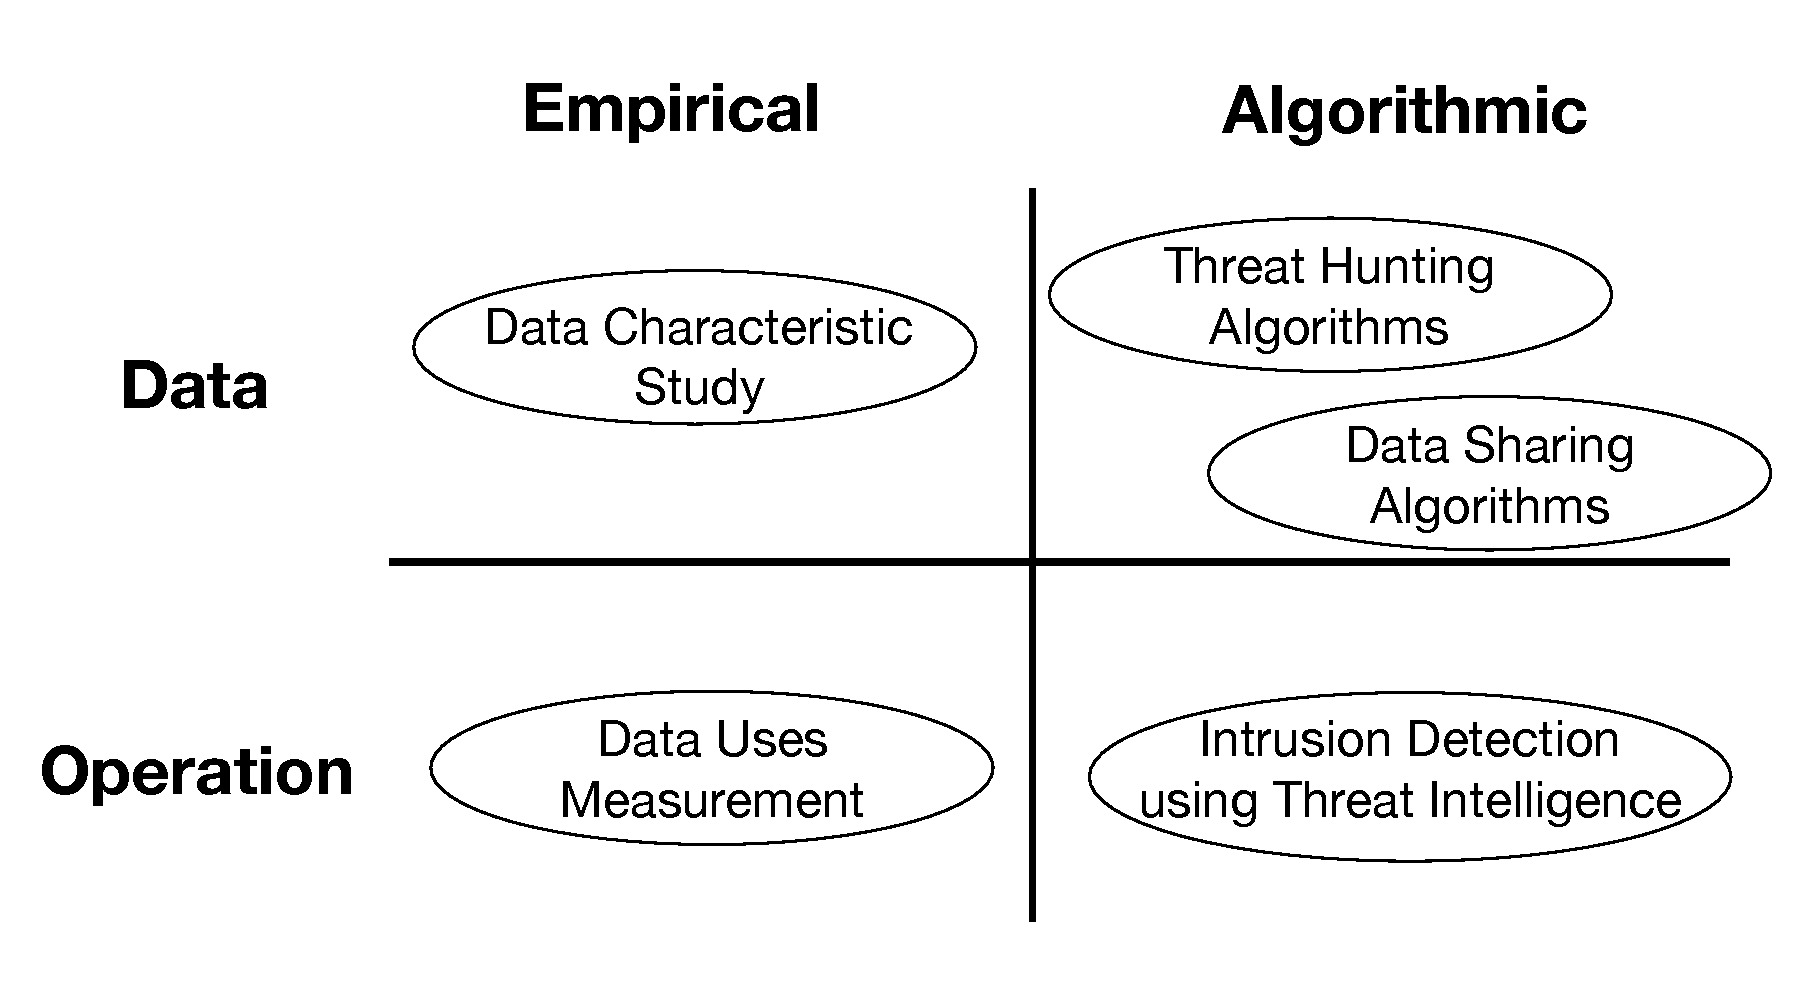
\includegraphics[width=0.8\textwidth]{threat_intel_research_overview.pdf}
\caption{Threat Intelligence research overview and example research
topics in each direction.}
\label{fig:threat_intel_overview}
\end{figure}

Therefore, research directions related to Threat Intelligence can be 
viewed in four general categories, as illustrated in
Figure~\ref{fig:threat_intel_overview}. More specifically, the four 
research directions are: 
\begin{prettylist}
    \item Empirical analysis on Threat Intelligence data: \\
    Understanding the characteristic of Threat Intelligence data, different
    data generation systems and their performance, different threat sharing
    strategies and how are they being used in the real-world, etc.
    
    \item Algorithm exploration related to Threat Intelligence data: \\
    Designing algorithms for threat hunting (Threat Intelligence generation),
    specification for data description and protocols for data sharing, etc.
    
    \item Empirical analysis on Threat Intelligence usage: \\
    Measuring how organizations are using Threat Intelligence, the problems 
    when using these data and the impact on the Internet, etc.
    
    \item Algorithm exploration related to Threat Intelligence usages: \\
    Designing better methods to use threat intelligence during system and 
    network defense(e.g. increasing coverage, reducing false positives),
    explore new ways to use threat intelligence data, such as using the 
    data as machine learning training data, etc.
\end{prettylist}

In this dissertation, I take an empirical approach and explore the 
\textit{Data} and \textit{Operation} problems of Threat Intelligence.
I focus on thoroughly understanding the current status of Threat 
Intelligence and will then discuss my takeaways from these analyses.
In the study of \textit{Data}, which will be discussed in Chapter~\ref{chapter:data_character}, 
I analyzed the data characteristics of existing Threat Intelligence products.
I designed mathematics metrics for Threat Intelligence data evaluation,
and with these metrics, I studied \numipfeeds\ distinct IP address 
data feeds, covering six categories of threats, and \numhashfeeds\ distinct
malware file hash feeds, and measured their data characteristic. Through this
work, I revealed the limitation of existing Threat Intelligence data and 
discussed the potential improvements based on my findings. In the study of
\textit{Operation}, which will be discussed in Chapter~\ref{chapter:data_usage},
I measured how Threat Intelligence data is being used on a large scale. 
I designed a method using IP ID side channel that can measure the 
connectivity between two Internet hosts from a third point. With this 
method, I conducted a large scale Internet measurement over {\reflroughnum} 
U.S. hosts and uncovered their uses of {\blacklistnum} popular public IP
blacklists. I further investigated a broader use of blacklists among the 
hosts, and discovered over 73K hosts has shown blacklist related blocking 
behavior. Together, my work provided an in-depth look into the current
status of Threat Intelligence and augmented the knowledge of our community
on this topic.

%\verb!\mainmatter! macro because it should start on page~1.
%\end{dissertationintroduction}

\section{Overview}
\label{sec:overview}

The threat intelligence data collected for this study was obtained by
subscribing to and pulling from numerous public and private 
intelligence sources. These sources ranged from simple blacklists of 
bad IPs/domains and file hashes, to rich threat intelligence exchanges 
with well labeled and structured data.
I refer each item (\eg IP address or file hash) an \emph{indicator}
(after \emph{indicator of compromise}, the industry term for such data items).

In this section, I enumerate the threat intelligence sources, describe
each source's structure and how I collected it, and then define our
measurement metrics for empirically measuring these sources.  When the
source of the data is public, or when I have an explicit agreement to
identify the provider, I have done so.  However, in other cases, the
data was provided on the condition of anonymity and I restrict
myself to only describe the nature of the provider, but not their
identity.  All of the private data providers were appraised of the
nature of my research, its goals and the methodology that I planned
to employ.


%\pp{Try to use feeds when describing all except FB and TS. I've reworked such
%that feeds -> sources}

\subsection{Data Set and Collection}

I use several sources of \ti\ data for my analysis:

\emphpar{Facebook ThreatExchange (FB)~\cite{FBThreatExchange}}
    This is a closed-community platform that allows hundreds of companies and
    organizations to share and interact with various types of labeled threat data.
    As part of an agreement with Facebook, I collected all its data that it shared broadly.
    In subsequent analyses, sources with
    prefix ``FB'' indicate a unique contributor on the Facebook ThreatExchange.

\emphpar{Paid Feed Aggregator (PA)} This is a commercial paid threat intelligence data aggregation
    platform. It contains data collected from over a hundred other
    threat intelligence sources, public or private, together with its own threat data.
    In subsequent analyses all data sources with prefix ``PA''
    are from unique data sources originating from this aggregator.

\emphpar{\feedetiprep\ Service} This commercial service provides an
    hourly-updated blacklist of known bad IP addresses across different attack categories.

\emphpar{Public Blacklists and Reputation Feeds} I collected indicators from public
    blacklists and reputation data sources, including well-known
    sources such as AlienVault~\cite{Alienvault}, Badips~\cite{Badips}, Abuse.ch~\cite{Abuse-ch}
    and Packetmail~\cite{Packetmail}.

Threat Intelligence indicators include different types of data, such as IP address, malicious file hash, Domain,
URL, etc. In this chapter, I focus the analysis on sources that provide IP addresses and file hashes,
as they are the most prevalent data types in my collection.

I collect data from all sources on an hourly basis. However, both the Facebook
ThreatExchange and the Paid Feed Aggregator change their members and contributions
over time, creating irregular collection periods for several of the sub-data sources.
Similarly, public threat feeds had varying degrees of reliability, resulting in
collection gaps. In this chapter, I use the time window from \veryemph{December 1, 2017}
to \veryemph{July 20, 2018} for most of the analyses, as I have the largest number
of active sources during this period. I eliminated duplicates sources (e.g., sources
we collected individually and also found in the {Paid Aggregator}) and
sub-sources (a source that is a branch of another source). I further break IP
sources into separate categories and treat them as individual feeds, as shown in
Section~\ref{sec:ip-analysis}. This filtering leaves us with \numipfeeds\ IP feeds and
\numhashfeeds\ malware file hash feeds.

The ways each \ti\ source collects data varies, and in some cases
the methodology is unknown. For example, {\feedpacketmail} and {\feedetiprep}
collect threat data themselves via honeypots, analyzing malware, etc. Other
sources, such as {Badips} or the Facebook ThreatExchange, collect their
indicators from general users or organizations---\eg\ entities may be attacked
and submit the indicators to these threat intelligence services. These services
then aggregate the data and report it to their subscribers. Through this level of
aggregation the precise collection methodologies and data
providence can be lost.


\subsection{Data Source Structure}
\label{sec:feed-structure}

\ti\ sources in my corpus structure and present data in different ways.
Part of the challenge in producing cross-dataset metrics is normalizing both
the structure of the data as well as its \emph{meaning}. A major structural
difference that influences my analysis occurs between data sources that
provide data in \emph{snapshots} and data sources that provide \emph{events}.

\emphpar{Snapshot}
Snapshot feeds provide periodic snapshots of a set of indicators. More formally, a
snapshot is a set of indicators that is a function of time. It defines, for a given point in
time, the set of indicators that are members of the data source. Snapshot feeds imply
\emph{state}: at any given time, there is a set of indicators that are \emph{in} the feed.
A typical snapshot source is a published list of IPs periodically updated by its maintainer.
For example, a list of command-and-control IP addresses for a botnet may be published as a
snapshot feed subject to periodic updates.

All feeds of file hashes are snapshots and are \emph{monotonic} in the sense that indicators
are only added, not removed, from the feed. Hashes are a proxy for the file
content, which does not change (malicious file content will not change to benign in the future).

\emphpar{Event}
In contrast, event feeds report newly discovered indicators. More formally, an event source
is a set of indicators that is a function of a time \emph{interval.} For a given time interval,
the source provides a set of indicators that were seen or discovered in that time interval.
Subscribers of these feeds query data by asking for new indicators added in a recent time window.
For example, a user might, once a day, request the set of indicators that appeared
in the last 24 hours.

This structural difference is a major challenge when evaluating feeds comparatively.
I need to normalize the difference to make a fair comparison, especially for IP feeds. From a \ti\
consumer's perspective, an \emph{event} feed does not indicate when an indicator will
expire, so it is up to the consumer to act on the age of indicators. Put another way,
the expiration dates of indicators are decided by how users query the feed:
if a user asks for the indicators seen in the last 30 days
when quering data, then there is an implicit 30-day valid time window for these indicators.

In this chapter, I choose a 30-day valid period for all the indicators I collected from event feeds---the same valid period
used in several snapshot feeds, and also a common query window option offered by event feeds.
I then convert these event feeds into snapshot feeds and evaluate all of them in a unified fashion.


\begin{comment}
Snapshot sources are build on a notion of emph{state}, namely, the current indicators
in the list at a certain moment, as indicators could be added and removed from
the source over time. This type of source mainly apply for IP feeds, as IP data
is time sensitive---a malicious IP address discovered now might not be malicious
in the future. One example of such source is {\feedfeodo}\cite{Feodo}, which records
a list of current Command and Control server IPs of Feodo botnet\cite{Feodo-Tracker}
that a site should block.

Event sources, on the other hand, is ``stateless'', they focus on what have been
discovered recently. One example of this type of source is {\feednothink}\cite{Nothink}.
Upon request, it returns the source IPs they collected that have conducted SSH
brute-force attack in the last day, last week or last year, depending on the specified
query option.

This structural difference doesn't concern file hash feeds, since file hashes are time
insensitive---a malicious file hash won't change to benign in the future. One can
think of all file hash feeds as snapshot feeds where indicators never expire.
\end{comment}

\subsection{Threat Intelligence Metrics}
\label{sec:metrics}

%\note{Should explain why each of these metrics is useful.}
The aim of this work is to develop \emph{threat intelligence metrics} that
allow a \ti\ consumer to compare threat intelligence sources and reason about
their fitness for a particular purpose. To this end, I propose six concrete
metrics: \emph{Volume}, \emph{Differential contribution}, \emph{Exclusive contribution},
\emph{Latency}, \emph{Accuracy} and \emph{Coverage}.

%\noteby{KL}{This needs to be updated to \emph{size} and \emph{rate}.}

\metrics \emphpar{Volume} I define the \emph{volume} of a feed to be the total
number of indicators appearing in a feed over the measurement interval. Volume
is the simplest \ti\ metric and has an established history in prior
work~\cite{jung2004empirical,kuhrer2014paint,
trajectory:oakland11,tasters:imc12,sheng2009empirical,sinha2008shades,thomas2016abuse}.
It is also useful to study the daily \emph{rate} of a feed, which quantifies
the amount of data appearing in a feed on a daily basis.

\emph{Rationale}: To a first approximation, volume captures how much
information a feed provides to the consumer. For a feed without false positives
(see \emph{accuracy} below), and if every indicator has equal value to the
consumer, one would prefer a feed of greater volume to a feed of lesser volume.
Of course, indicators do not all have the same value to consumers: knowing the
IP address of a host probing the entire Internet for decades-old
vulnerabilities is less useful than the address of a scanner targeting
organizations in your sector looking to exploit zero-day vulnerabilities.

\metrics \emphpar{Differential contribution} The \emph{differential
contribution} of one feed with respect to another is the number of indicators
in the first that are not in the second during the same measurement period. We
define differential contribution relative to the size of the first feed, so
that the differential contribution of feed $A$ with respect to feed $B$ is
$\mathrm{Diff}_{A,B} = |A \setminus B|/|A|$. Thus, $\mathrm{Diff}_{A,B}=1$
indicates that the two feeds have no elements in common, and
$\mathrm{Diff}_{A,B} = 0$ indicates that every indicator in $A$ also appears in
$B$. It is sometimes useful to consider the complement
of differential contribution, namely the normalized \emph{intersection} of $A$ in $B$,
given by $\mathrm{Int}_{A,B} = |A \cap B|/|A| = 1-\mathrm{Diff}_{A,B}$.

%(Figure~\ref{fig:overall_heatmap}, in Section~\ref{sec:ip-overlap}, for
%example, shows intersection rather than differential contribution, following the
%Taster's Choice convention.)

\emph{Rationale}: For a consumer, it is often useful to know how many \emph{additional}
indicators a feed offers relative to one or more feeds that the consumer has already.
Thus, if a consumer already has feed $A$ and is considering paying for feed $B$,
then $\mathrm{Diff}_{A,B}$ indicates how many new indicators feed $A$ will provide.

\metrics \emphpar{Exclusive contribution} The \emph{exclusive contribution} of
a feed with respect to a set of other feeds is the proportion of indicators
unique to a feed, that is, the proportion of indicators that occur in the feed
but no others. Formally, the exclusive contribution of feed $A$
is defined as $\mathrm{Uniq}_{A,B} = |A \setminus \bigcup_{B\neq A}B|/|A|$.
Thus, $\mathrm{Uniq}_{A,B} = 0$ means that every element of feed $A$ appears in
some other feeds, while $\mathrm{Uniq}_{A,B}=1$ means no element of $A$ appears
in any other feed.

%Exclusive contribution was first described for domain feeds
%in Taster's Choice~\cite{tasters:imc12}.

\emph{Rationale}: Like differential contribution, exclusive contribution tells
a \ti\ consumer how much of a feed is different. However, exclusive contribution
compares a feed to all other feeds available for comparison, while differential
contribution compares a feed to just another feed. From a \ti\ consumer's
perspective, exclusive contribution is a general measure of a feed's unique
value.
%A feed that aggregates several other feeds may have no exclusive
%contribution, but may provide great value to a consumer.

\metrics \emphpar{Latency} For an indicator that occurs in two or more feeds, its
\emph{latency} in a feed is the elapsed time between its first appearance in any
feed and its appearance in the feed in question. In the feed where an indicator
first appeared, its latency is zero. For all other feeds, the latency indicates
how much later the same indicators appears in those feeds. Taster's
Choice~\cite{tasters:imc12} referred to latency as \emph{relative first appearance
time}. (I find the term \emph{latency} to be more succinct without loss of
clarity.) Since latency is defined for one indicator, for a feed it makes sense
to consider statistics of the distribution of indicator latencies, such as the
median indicator latency.

\emph{Rationale}: Latency characterizes how quickly a feed includes new
threats: the sooner a feed includes a threat, the more effective it is at
helping consumers protect their systems. Indeed, several studies report on the
impact of feed latency on its effectiveness at
thwarting spam~\cite{blacklisting:weis14,ramachandran2007filtering}.

The metrics above are defined without regard for the \emph{meaning} of the
indicators in a feed. One can calculate the volume of a single feed or the
differential contribution of one feed with respect to another regardless of
what the feed purports to contain. While these metrics are easy to compute,
they do little to tell us about the fitness of a feed for a particular purpose.
For this, I need to consider the meaning or purpose of the feed data, as
advertised by the feed provider. I define the following two metrics.

\metrics \emphpar{Accuracy} The \emph{accuracy} of a feed is the proportion of
indicators in a feed that are correctly included in the feed. Feed accuracy is
analogous to \emph{precision} in Information Retrieval. This metric presumes
that the description of the feed is well-defined and describes a set of elements
that should be in the feed given perfect knowledge. In practice, 
researchers have neither
perfect knowledge nor a perfect description of what a feed should contain. In
some cases, however, I can construct a set $A^-$ of elements that should
definitely not be in a feed $A$. Then $\mathrm{Acc}_A \le |A\setminus A^-|/|A|$.

\emph{Rationale}: The accuracy metric tells a \ti\ consumer how many false
positives to expect when using a feed, and, therefore, dictates how a feed
can be used. For example, if a consumer automatically blocks all traffic to
IP addresses appearing in a feed, then false positives may cause disruption
in an enterprise by blocking traffic to legitimate sites. On the other hand,
consumers may tolerate some false positives if a feed is only used to
gain additional insight during an investigation.

\metrics \emphpar{Coverage} The \emph{coverage} of a feed is the proportion
of the intended indicators contained in a feed. Feed coverage is analogous
to \emph{recall} in Information Retrieval. Like accuracy, coverage presumes
that the description of the feed is sufficient to determine which elements
should be in a feed, given perfect knowledge. In some cases, it is possible
to construct a set $A^+$ of elements that should be in a feed. I can then
upper-bound the coverage $\mathrm{Cov}_A \le |A|/|A^+|$.


\emph{Rationale}: For a feed consumer who aims to obtain complete protection
from a specific kind of threat, coverage is a measure of how much protection
a feed will provide. For example, an organization that wants to protect itself
from a particular botnet will want to maximize its coverage of that botnet's
command-and-control servers or infection vectors.

In the following two sections, I use these metrics to evaluate two types of
\ti: IP address feeds and file hash feeds.

\section{IP Threat Intelligence}
\label{sec:ip-analysis}

One of the most common forms of \ti\ are feeds of IP addresses considered malicious,
suspicious, or otherwise untrustworthy. This type of threat intelligence dates back
at least to the early spam and intrusion detection blacklists, many of which are
still active today such as SpamhausSBL~\cite{SpamhausSBL}, CBL~\cite{CBL} and
SORBS~\cite{SORBS}. Here, we apply the metrics described above to quantify the
differences between \numipfeeds\ different IP address \ti\ feeds.
%The overview of the these feeds is summarized in Table~\ref{tab:volume-overview-1}.


\subsection{Feed Categorization}
IP address \ti\ feeds have different meanings, and, therefore, purposes. To
meaningfully compare feeds to each other, we first group feeds into
\emph{categories} of feeds whose indicators have the same intended meaning.
Unfortunately, there is no standard or widely accepted taxonomy of IP \ti\ feeds.
To group feeds into semantic categories, we use metadata associated with the
feed as well as descriptions of the feed provided by the producer, as described below.

\emphpar{Metadata} Some feeds provide category information with each indicator as
metadata. More specifically, all of the {Paid Aggregator} feeds, {\feedalienvault}
and {\feedetiprep} include this category metadata. In this case, we use its pre-assigned
category in the feed. Facebook ThreatExchange feeds do not include category
information in the metadata, but instead provide a descriptive phrase with each indicator.
We then derive its category based on the description.

\emphpar{Feed description} For feeds without metadata, we rely on online descriptions
of each feed, where available, to determine its semantic category. For example, the
website of feed {\feednothink}~\cite{Nothink} describes that the feed reports brute-force
login attempts on its corresponding honeypot, which indicates the feed belongs to
brute-force category.

We grouped our IP feeds into categories derived from the information
above. In this work, we analyze six of the most prominent categories:
%, listed below.
%
\begin{categorylist}\small
\item[Scan] Hosts doing port or vulnerability scans.
\item[Brute-force] Hosts making brute force login attempts.
\item[Malware] Malware C\&C and distribution servers.
\item[Exploit] Hosts trying to remotely exploit vulnerabilities.
\item[Botnet] Compromised hosts belonging to a botnet.
\item[Spam] Hosts that sent spam or should not originate email.
\end{categorylist}
%
Table~\ref{tab:volume-overview-1} lists the feeds, grouped by category, used in the
rest of this section. The symbols \snapfeedsym\ and \deltafeedsym\ before the feed
name indicate whether the feed is a snapshot feed or an event feed, respectively
(see Section~\ref{sec:feed-structure}).
All data was collected during our measurement period,
\veryemph{December 1st, 2017} to \veryemph{July 20th, 2018}. Note that a few
feeds, like {\feedetiprep}, appear in multiple categories. In these feeds, indicators
are associated with different categories via attached metadata. We split these feeds
into multiple virtual feeds each containing indicators belonging to the same category.

\subsection{Volume}
\label{sec:ip-volume}

%\noteby{KL}{Change this to Size and Rate.}
Volume is one of the oldest and simplest \ti\ metrics representing how informative
each data source is. Table~\ref{tab:volume-overview-1} and Table~\ref{tab:volume-overview-2} shows the total number of unique IP addresses
collected from each feed during the measurement period, under column \emph{Volume}. A \snapfeedsym\ denotes a \textit{snapshot feed}
and \deltafeedsym\ indicates an \textit{event feed} (Section~\ref{sec:feed-structure}).
\colname{Volume} is the total number of IPs collected during our measurement period.
\colname{Exclusive} is the exclusive contribution of each feed (Section~\ref{sec:ip-unique}).
\colname{Avg. Rate} is the number of average daily new IPs added in the feed (Section~\ref{sec:ip-accuracy}), and
\colname{Avg. Size} is the average working set size of each feed (Section~\ref{sec:ip-volume}).
Feeds are listed in order of decreasing volume, grouped by category.
The numbers we show are after the removal of invalid entries identified
by the sources themselves. Column \emph{Avg. Rate} shows the average number of
new IPs we received per day, and \emph{Avg. Size} lists the average daily
working set size of each feed, that is, the average size of the snapshot.

\finding\ Feeds vary dramatically in volume. Within every category, big feeds can contain
orders of magnitude more data than small feeds. For example, in the scan category, we saw
over 361,004 unique IP addresses in \feeddshield\ but only 1,572 unique addresses
in \feedTSAnalyst\ in the same time period. Clearly, volume is a major differentiator
for feeds. %In Section~\ref{sec:ip-overlap} and~\ref{sec:ip-unique}, we will examine which
%feeds duplicate each other and which feeds contribute unique indicators.

\input{data_character/content/ip-volume-table}


Average daily rate represents the amount of new indicators collected from a feed each day.
Some feeds may have large volume but low daily rates, like {\feedfeodo} in the malware
category. This means most indicators we get from that feed are old data present in the feed before our
measurement started. On the other hand, the average rate of a feed could be
greater than the volume would suggest, like {\feednothink} in the brute-force category.
This is due to the fact that indicators can be added and removed multiple times in a
feed. In general, IP indicators tend to be added in a feed only once: 37 among \numipfeeds\
IP feeds have over 80\% of their indicators appearing only once, and 30 of them have this rate over 90\%.
One reason is that some snapshot feeds maintain a valid period for each indicator, as
we found in all \emph{PA} feeds where the expiration date of each indicator is explicitly
recorded. When the same indicator is discovered again by a feed before its expiration time,
the feed will just extend its expiration date, so this occurrence will not be captured
if we simply subtract the old data from the newly collected data to derive what is added on a day.
For event feeds and snapshot feeds in \emph{PA} where we can precisely track every occurrence
of each indicator, we further examed data occurrence frequency and still found that the vast
majority of IPs in feeds only occurred once---an observation that relates to the dynamics
of cyber threats themselves.

\feednothink, as we mentioned above, is a notable exception. It has over 64\% of its
indicators appearing 7 times in our data set. After investigating, we
found that this feed posts all its previous data at the end of every month, behavior very likely
due to the feed provider instead of the underlying threats.
% {\feedusername}, {\feedbadipftp}, {\feedbadipdns} and {\feedbadipsql}
% all have a large percent of IPs appeared twice, and we found
% that all 4 feeds reported a abnormally large amount of same IPs on 2018 July 1st and July 13th.
% We will discuss more about this in Section~\ref{sec:ip-accuracy}.

The working set size defines the daily average amount of indicators users need to store in their
system to use a feed (the storage cost of using a feed). The average
working set size is largely decided by the valid period length
of the indicators, controlled either
by the feed (snapshot feeds) or the user (event feeds). The longer the valid period is,
the larger the working set will be. Different snapshoot feeds have different choices for this
valid period: {\feedTSAlienVault} in the scan category sets a 90-day valid period for
every indicator added to the feed, while {\feedTSAbusech} uses a 30-day period. Although we do not
know the data expiration mechanism used by snapshot feeds other than \emph{PA} feeds, as
there is no related information recorded, we can still roughly estimate this by checking the
\emph{durations} of their indicators---the time between an indicator being added and being removed.
Four {\feedetiprep} feeds have more than 85\% of durations shorter than 10 days, while the one in
the malware category has more than 40\% that span longer than 20 days. {\feedfeodo} has over 99\% of
its indicators valid for our entire measurement period, while over 70\% of durations in the
{\feedzeus} are less than 6 days. We did not observe a clear pattern regarding how each snapshot
feed handles the expiration of indicators.

%The column \emph{Occurred} presents the number of unique IPs added in a \ti\ source after our
%measurement period started. We differentiate \emph{Volume} and \emph{Occurred} since IP
%indicators are time sensitive: They are added, removed and could be added again in a feed over
%time. When we pull data from a snapshot feed on a day, some IPs are actually added
%on previous days and are still kept by the feed. \emph{Occurred} only captures the IPs that
%are newly added after the measurement period started, while \emph{Volume} includes legacy data in
%a feed when we collect indicators on the first day of our analysis. At a high level,
%\emph{Volume} represents the number of IPs that a feed \emph{considers} as malicious during
%a period of time, and \emph{Occurred} represents the number of newly discovered indicators by the
%feed during that time.

%For delta feeds, we calculated their \emph{Volume} by tracking the expiration dates of the
%indicators we collected before (The expiration dates are provided in the metadata) and included
%the indicators whose expiration dates are after January 1st, 2016.

\subsection{Differential Contribution and Intersection}
\label{sec:ip-overlap}

%It is often useful to know whether a potential new feed contributes any new indicators relative to what a \ti\ consumer has already.
The differential contribution metric measures the number of indicators in one feed that are not in another. Equivalently, we can consider the intersection of two feeds, which is the number of elements in one feed that are present in the other, normalized by the size of the first: $|A\cap B|/|A|$. Figure~\ref{fig:overall_heatmap} shows the intersection relationship of all feeds in the study. Each cell in the matrix represents the number of elements in both feeds, normalized by the size of the feed spanning the rows on the table. That is, $A$, in the expression above, ranges over rows, and $B$ over columns of the matrix. Darker (more saturated) colors indicate greater intersection. Comparisons of feeds within a category are shaded red and comparisons of feeds between different categories are shaded blue. Note that the matrix is asymmetric, because, in general, $|A\cap B|/|A| \neq |A\cap B|/|B|$. Elements of the matrix are in the same order as in Table~\ref{tab:volume-overview-1}.

\begin{figure}
\centering
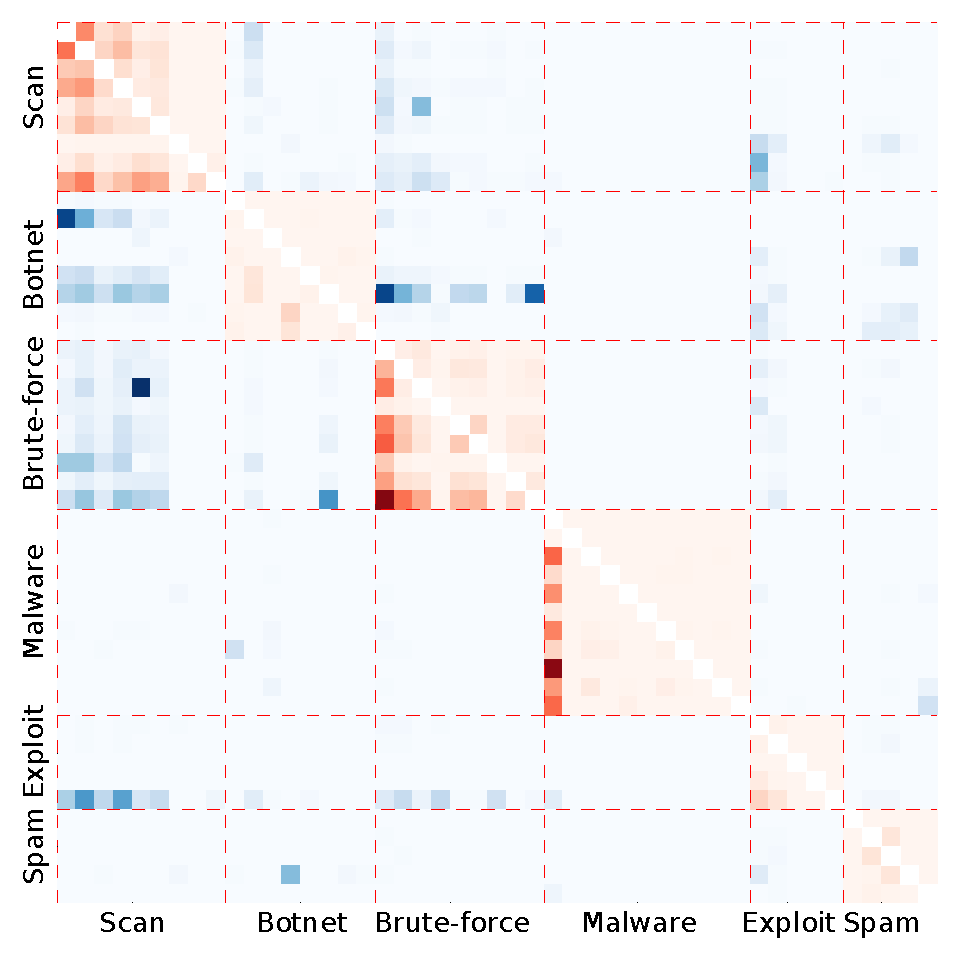
\includegraphics[width=0.475\textwidth]{images/overall_heatmap.pdf}
\caption{Feed intersection for all IP feeds. Each row/column represents a feed, shown in the same order as Table~\ref{tab:volume-overview-1}. Darker (more saturated) colors indicate greater intersection.}
\label{fig:overall_heatmap}
\end{figure}

%\begin{figure}
%\centering
%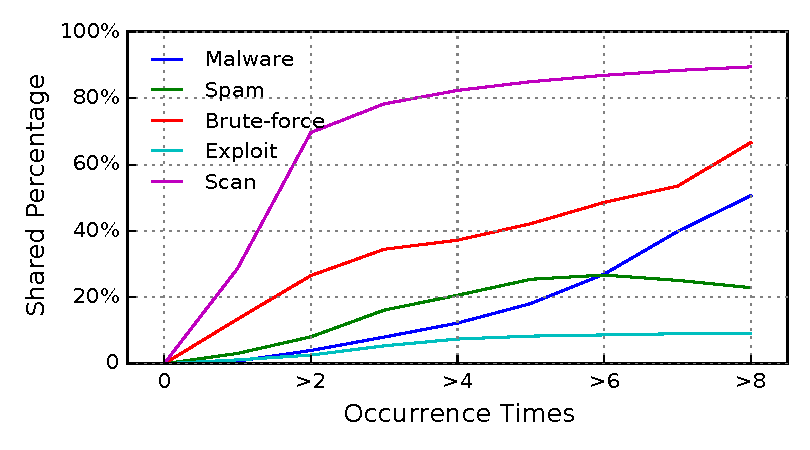
\includegraphics[width=0.4\textwidth]{images/occur_vs_overlap.pdf}
%\caption{Relation between indicators' occurrence frequency and the percentage of being shared. Each point on a line means: For the %indicators that had occurred >\emph{x} times in a feed(\textbf{X} axis), how much percent of them are shared among at least two feeds within its category(\textbf{Y} axis).}
%\label{fig:occur_vs_overlap}
%\end{figure}

\finding\ Feeds in scan and brute-force categories have higher pairwise intersections: Half of the pairwise intersection rates in two categories are greater than 5\%. The scan category has 29 out of 72 pairs (excluding self comparisons) with an intersection rate larger than 10\%, and the same case occurred in 19 out of 72 pairs in the brute-force category.

On the other side, feeds in the botnet, exploit, malware and spam category do not share much data between each other: all 4 categories have more than three-quarters of pairwise intersection rates less than 1\%. A few big feeds in these categories can share a significant amount of data with some small feeds in the same category---a characteristic that appears as a dark vertical line within its category in Figure~\ref{fig:overall_heatmap}. \feedetiprep\ in the malware category, for example, shares over 30\% of 6 other malware feeds. But the intersections among the vast majority of feeds in these 4 categories are low. This finding is consistent with prior work~\cite{metcalf2015blacklist,thomas2016abuse}, but we provide a more comprehensive view regarding different categories.

Figure~\ref{fig:overall_heatmap} also shows the relation between feeds across different categories. We can clearly see a relation between scan and brute-force feeds: multiple scan feeds have non-trivial intersection with feeds in the brute-force category. In fact, 23.1\% of all 760,263 brute-force IPs we collected are also included by scan feeds in our dataset. There are also three botnet feeds---\feedTSCI, \feedTSVoIP\ and \feedTSCompr---that have over 10\% of its data shared with multiple feeds in the scan category.

%\noteby{KL}{Cut this paragraph and accompanying figure.}
%One interesting question is: Are indicators that occurred multiple times in a feed more likely to be shared between feeds? We check this question by calculating how much percent of indicators, that had occurred more than \emph{x} times in a feed, are shared between at least two feeds within each category. The result is shown in Figure~\ref{fig:occur_vs_overlap}. Botnet category is excluded from the Figure since the percentages are too low to argue about the trend. We can see that there is a strong positive correlation between the occurrence frequency and the percentage being shared, across different categories. This aligns with the intuition that a persistent attacker is more likely being observed by mulitple \ti\ sources.

\subsection{Exclusive Contribution}
\label{sec:ip-unique}

Exclusive contribution represents the number of indicators in a feed that are in no other feeds. I calculate each feed's exclusive contribution among all the feeds in the same category, emphasizing their uniqueness regarding the scope of data they claim to report. Each feed's exclusive contribution is presented in Table~\ref{tab:volume-overview-1} in column \emph{Exclusive}, calculated based on its volume.

\finding\ As I already observed in Section~\ref{sec:ip-overlap}, botnet, exploit and spam feeds have relatively low pairwise intersections. Consequently, the feeds in these four categories have high exclusive contribution rates in general: the median exclusive contribution rates of these four categories are 90.9\%, 97.5\% and 90.5\%, respectively. The malware category has a low median exclusive rate, since multiple small feeds have non-trivial intersection with the largest feed {\feedetiprep}, but the two largest feeds in malware both have a exclusive rate over 99\%. Scan and brute-force feeds have more intersection within its category, and their exclusive rates are lower: 62.0\% median rate in scan and 62.7\% in brute-force, and the top two largest feeds in both categories have an exclusive rate below 85\%.

If one assumes a process where a feed is more likely to have popular elements, then smaller feeds would be subsumed by larger feeds. Yet, for some small feeds like {\feedmalcode} in the malware and {\feedTSHoneypot} in the botnet categories, even though they are several orders of magnitude smaller than the largest feeds in their categories, a significant proportion of their indicators is still unique to the feed. When I aggregate the data in each category, 73\% of all scan feed indicators are unique to a single feed and 88\% of brute force feed indicators are unique to one feed. For other categories, over 97\% of elements in the category are unique to a single feed. This result agrees with previous work that most data in threat intelligence feeds is unique~\cite{metcalf2015blacklist,thomas2016abuse}.
\subsection{Latency}
\label{sec:ip-timing}

% Data Occurrence analysis
Feed latency measures how quickly a feed reports new threat indicators. The
sooner a feed can report potential threats, the more valuable it is for
consumers. The absolute latency of an indicator in a feed is the time from
the beginning of the corresponding event until when the indicator shows up in
the feed. However, it is difficult to know the actual time when an event begins
from the threat intelligence data. Instead, we measure the \textit{relative
latency}, which is the delay of an indicator in one feed to be the time between
its appearance in that feed and the first seen among all the feeds.

\begin{figure}[t!]
\centering
\subfloat[Latency distribution in scan feeds]{
	\label{fig:scan_firstseen}
	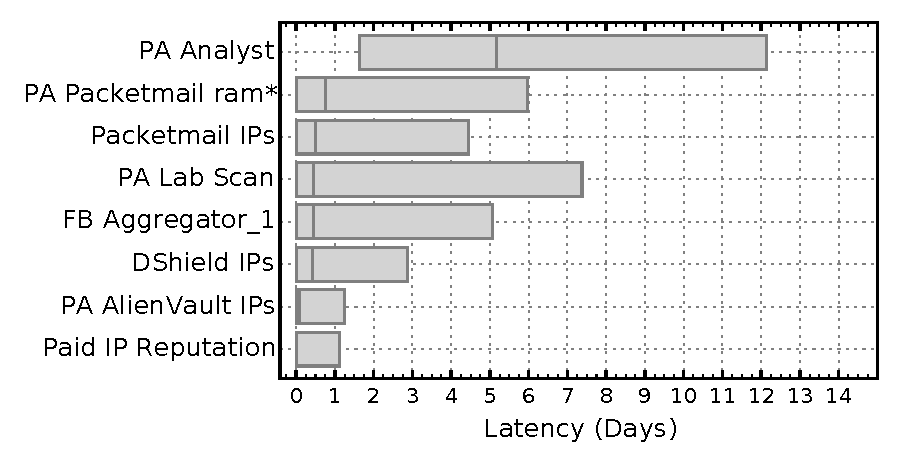
\includegraphics[width=0.8\textwidth]{data_character/images/scan_latency_new.pdf}}

\subfloat[Latency distribution in brute-force feeds]{
	\label{fig:brute_firstseen}
	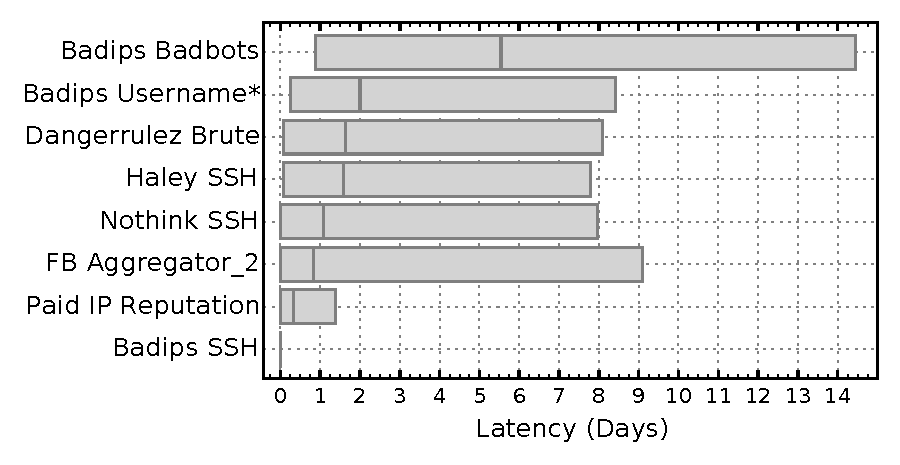
\includegraphics[width=0.8\textwidth]{data_character/images/brute_latency_new.pdf}}

\caption{Distribution of indicators' latency in scan and brute-force feeds.}
\label{fig:firstseen}
\end{figure}


Relative latency can only be calculated for
indicators that occur in at least two feeds. As discussed in
Section~\ref{sec:ip-unique}, the number of common indicators in the botnet, malware, exploit and spam feeds is very low (fewer than 3\% of elements occur in more than one feed). Relative latency calculated for these feeds is less meaningful. For this analysis, therefore, we focus on scan and brute-force feeds.

Another issue is the time sensitivity of IP threats. An event that originated from
an IP address, like scanning activity or a brute-force attack, will not last
forever. If one scan feed reports an IP address today and another feed reports
the same IP three months later, it would make little sense to consider them as one
scanning event and label the second occurrence as being three months late.
Unfortunately, there is no easy way we can clearly distinguish events from each
other. Here we use a one-month window to restrict an event, assuming that the same
attack from one source will not last for more than 30 days; although arbitrary, it provides a reasonably conservative threshold, and experimenting with other thresholds produced similar overall results. More specifically, we calculate relative latency by tracking the
first occurrence of IPs in all feeds in a category, then recording the latency of the
following occurrences while excluding ones that occur after 30 days. By just
using the first appearance of each IP as the base, we avoid the uncertainty caused by
multiple occurrence of indicators and different valid periods used among feeds.

%We also used other time windows for the latency calculation and the results are very similar.

Figures~\ref{fig:scan_firstseen} and~\ref{fig:brute_firstseen} show the relative
latency distribution among feeds in the scan and brute-force categories, in hours. Each box shows the latency distribution of shared IPs in the feed calculated in hours
from 25 percentile to 75 percentile, with the middle line indicating the median.
(``Badips Username*'' here is the abbreviation for feed name Badips
Username Notfound; ``PA Packetmail Ram*'' for PA Packetmail Ramnode)
We focus on just those feeds that have
over 10\% of their data shared with others to ensure the analysis can represent the latency
distribution of the overall feed. There is one feed in each category ({\feedTSSnort}
in scan and {\feedTSBrute} in brute-force) that is excluded from the figure.

\finding\
From the distribution boxes we can see that {\feedetiprep} in scan and {\feedbadipssh}
in brute-force are the fastest feeds in their category, as they have the lowest median
and 75th percentile latencies. On the other hand, {\feedTSAnalyst} in scan and
{\feedbadipbot} in brute-force are the slowest feeds. Figure~\ref{fig:scan_firstseen}
shows that all scan feeds except one have their 25th percentile latency equal to 0, indicating
these feeds, across different sizes, all reported a significant portion of their shared
data first. A similar case also happens in the brute-force category.

%This means that feeds can scan feeds, no matter fast or slow,

One may reasonably ask whether large feeds report data sooner than small feeds.
The result shows that this is not always the case. {\feedFBBasecamp} is the second smallest
feed in our scan category, yet it is no slower than several other feeds which have over 10 times of its daily rate.
{\feedbadipbot}, on the other hand, has the second largest rate in brute-force
category, but it is slower than all the other feeds in the brute-force category. Feeds that are small in volume can still report a lot of their data first.

% This shows that when choosing a feed, we cannot assume its latency by just looking at its volume.

Another factor that could affect latency is whether feeds copy data from each other. For example, 93\% of {\feeddangerrule} also appears in {\feedbadipssh}. If this is the case, we expect {\feeddangerrule} will be faster than {\feedbadipssh} on
reporting their shared data. However, we compared the relative latency between just two feeds and found {\feedbadipssh} reported 88\% of their shared indicators first.
We further conducted this pairwise latency comparison between all feeds in scan, brute-force
and malware (since {\feedetiprep} shares non-trivial amount of data with a
few small feeds in the malware category), and did not see a clear latency advantage between
any two feeds. Note that this observation does \emph{not} prove there is no data
copying, since the shared data between two feeds might partially come from copying and partially from the feeds' own data collection. Furthermore, our latency analysis is at a one-hour granularity.
% We did not find the evidence in latency to prove that there is indeed data copying.

\subsection{Accuracy}
\label{sec:ip-accuracy}
\input{data_character/content/ip-false-table}

Accuracy measures the rate of false positives in a feed. A false
positive is an indicator that data is labeled with a category to which
it does not belong.  For example, an IP address found in a scan feed
that has not conducted any Internet scanning is one such false
positive.  As well, even if a given IP is in fact associated with
malicious activity, if it is not unambiguously actionable (e.g.,
Google's DNS at 8.8.8.8 is used by malicious and benign software
alike) then for many use cases it must also be treated as a false
positive.  False positives are problematic for a variety of reasons,
but particularly because they can have adverse operational
consequences.  For example, one might reasonably desire to block all
new network connections to and from IP addresses reported as hosting
malicious activity (indeed, this use is one of the promises of threat
intelligence). False positives in such feeds, though, could lead to
blocking legitimate connections as well.  Thus, the degree of accuracy
for a feed may preclude certain use cases.

Unfortunately, determining which IPs belong in a feed and which do not
can be extremely challenging. In fact, at any reasonable scale, I am
unaware of any method for unambiguously and comprehensively
establishing ``ground truth'' on this matter.  Instead, in this
section I report on a proxy for accuracy that provides a
conservative assessment of this question.  To wit, I assemble a
\emph{whitelist} of IP addresses that either should not reasonably be
included in a feed, or that, if included, would cause significant
disruption. The presence of such IPs in a feed are
clearly false positives and thus define an upper bound on a feed's
accuracy.  I populate my list from three sources: unroutable IPs,
IPs associated with top Alexa domains, and IPs of major content
distribution networks (CDNs). The detail result for the accuracy analysis 
is presented in Table~\ref{tab:accuracy-overview-1} and 
Table~\ref{tab:accuracy-overview-2}.
\colname{Unrt} is fraction of unroutable addresses in each feed
(Section~\ref{sec:ip-accuracy}).
\colname{Alexa Top} is the number of IPs intersected with top Alexa domain 
IP addresses, and \colname{CDNs} is the number of IPs intersected with 
top CDN provider IP addresses. I will explain more about each column in below.

\noindent\textbf{Unroutable IPs.} Unroutable IPs are IP addresses that
were not BGP-routable \emph{when they first appeared} in a feed, as
established by contemporaneous data in the RouteViews
service~\cite{Routeview}. While such IPs could have appeared in the
source address field of a packet (i.e., due to address spoofing), it
would not be possible to complete a TCP handshake. Feeds that imply
that such an interaction took place should not include such IPs. For
example, feeds in the Brute-force category imply that the IPs they
contain were involved in brute-force login attempts, but this could
not have taken place if the IPs are not routable. While including
unroutable addresses in a feed is not, in itself, a problem, their
inclusion suggests a quality control issue with the feed, casting
shade on the validity of other indicators in the feed.

To allow for some delays in the feed, I check if an IP was routable
at any time in the seven days prior to its first appearance in a feed,
and if it had, I do not count it as
unroutable. Table~\ref{tab:accuracy-overview-1}, column \textit{Unrt},
shows the fraction of IP indicators that were not routable at any time
in the seven days prior to appearing in the feed. This analysis is
only conducted for the IPs that are added after my measurement
started. The number of such IPs is shown in column \textit{Added}, and
the unroutable fraction shown in \textit{Unrt} is with respect to this
number.

\noindent\textbf{Alexa.} Blocking access to popular Internet sites or
triggering alarms any time such sites are accessed would be disruptive
to an enterprise. For my analysis, I periodically collected the
Alexa top 25 thousand domains (3--4 times a month) over the course of
the measurement period~\cite{alexa}. To address the challenge that
such lists can have significant churn~\cite{scheitle2018long}, we
restrict my whitelist to hold the \emph{intersection} of all these
top 25K lists (i.e., domains that were in the top 25K every time we
polled Alexa over the 8-month measurement period), which left us with
12,009 domains. I then queried DNS for the A records, NS
records and MX records of each domain, and collected the corresponding
IP addresses. In total, I collected 42,436 IP addresses associated
with these domains. I compute the intersection of these IPs
with \ti\ feeds and show the results in column \textit{Alexa} in
Table~\ref{tab:accuracy-overview-1}.


\noindent\textbf{CDNs.} CDN providers serve hundreds of thousands of
sites. Although these CDN services can (and are) abused to conduct
malicious activities~\cite{cdnabuse}, their IP addresses are not
actionable.  Because these are fundamentally shared services,
blocking such IP addresses will also disrupt access to benign
sites served by these IPs.  I collected the IP ranges used by 5
popular CDN providers: AWS CloudFron~\cite{cloudfront},
Cloudflare~\cite{cloudflare}, Fastly~\cite{fastly},
EdgeCast~\cite{edgecast} and MaxCDN~\cite{maxcdn}. I then check how
many IPs in \ti\ feeds fall into these ranges. Column \textit{CDNs} in
Table~\ref{tab:accuracy-overview-1} shows the result.

\finding\ Among the \numipfeeds\ feeds in the table, 33 feeds have at
least one unroutable IP, and for 13 of them, over 1\% of the addresses
they contain are unrouteable. Notably, the {\feedetiprep} feed in the
spam category has an unroutable rate over 78\%.  Although it is not
documented, a likely explanation is that this feed may include unroutable
IPs intentionally, as this is a known practice among certain spam
feeds. For example, the Spamhaus DROP List~\cite{Spamhaus} includes IP
address ranges known to be owned or operated by malicious actors,
whether currently advertised or not. Thus, for feeds that explicitly
do include unroutable IPs, their presence in the feeds should not
necessarily be interpreted as a problem with quality control.

I further checked feeds for the presence of any ``reserved IPs''
which, as documented in RFC 8190, are not globally routable (e.g., private
address ranges, test networks, loopback and multicast).  Indeed,
12 feeds reported at least one reserved IP, including four of the
{\feedetiprep} feeds (excepting the spam category), six of the Badips
feeds, and the {\feedFBAdmin} and {\feeddshield} feeds. Worse, the
{\feedetiprep} feeds together reported over 100 reserved IPs. Since
such addresses should never appear on a public network,
reporting such IPs indicates that a feed provider fails to
incorporate some basic sanity checks on its data.

There are 21 feeds that include IPs from top Alexa domains, as shown
in column \textit{Alexa} in Table~\ref{tab:accuracy-overview-1}. Among
these IPs there are 533 A records, 333 IPs of MX records and 63 IPs of
NS records.  The overlapped IPs include multiple instances from
notable domains. For example, the IP addresses of www.github.com are
included by {\feedmalcode}.  {\feedetiprep} in the malware category
contains the IP address for www.dropbox.com.  {\feedalienvault}
contains the MX record of groupon.com, and {\feedbadipssh} also
contains the IP addresses of popular websites such as www.bing.com.

Most of the feeds I evaluated do not contain IPs in CDN ranges, yet
there are a few (including multiple {\feedetiprep} feeds, Badips feeds
and {\feedalienvault}) that have significant intersection with CDN
IPs. {\feedalienvault} and Badips feeds primarily intersect with
%IPs from
Cloudflare CDN, while most of the overlap in the {\feedetiprep} malware
category overlaps with AWS CloudFront.

Overall, the rate of false positives in a feed is not strongly
correlated with its volume.  Moreover, certain classes of false
positives (e.g., the presence of Top Alex IPs or CDN IPs) seem to
be byproducts of how distinct feeds are collected (e.g., Badips
feeds tend to contain such IPs, irrespective of volume).
Unsurprisingly, I also could find not correlation between a feed's
latency and its accuracy.
\subsection{Coverage}
\label{sec:completeness}

The coverage metric provides a quantitative measure of how well a
feed captures the intended threat. A feed with perfect
coverage would include all indicators that belong in a category.
Unfortunately, as discussed above, there is no systematic way for
evaluating the exact accuracy or coverage of a feed since it is unrealistic
to obtain ground truth of all threat activities on the Internet.

However, there are some large-scale threat activities that are
well-collected and well-studied. One example is Internet
scanning. Researchers have long been using ``Internet telescopes'' to
observe and measure network scanning
activities~\cite{benson2015leveraging, durumeric2014internet,
  pang2004characteristics}.  With a large telescope and well-defined
scan filtering logic, one can obtain a comprehensive view of global
scanning activities on the Internet.

To this end, we collected three months of traffic (from January 1st to
March 31st 2018) using the UCSD network telescope~\cite{telescope},
which monitors a largely quiescent /8 network comprising over 16
million IP addresses.  We then used the default parameters of the Bro
IDS~\cite{BroNetwork} to identify likely scanning traffic, namely
flows in which the same source IP address is used to contact 25 unique
destination IP addresses on the same destination port/protocol within
5 minutes. Given the large number of addressed being monitored, any
indiscriminate scanner observed by \ti\ feeds will likely also be seen
in our data.  Indeed, by intersecting against this telescope data we
are able to partially quantify the coverage of each \ti\ scanning feed.


%(u'TS Alien Vault OTX Malicious IPs', 'scan') 0.966922702159 0.0045119148556
%(u'dshield-ips', 'scan') 0.951590802754 0.00826350821018
%(u'TS Packetmail iprep ramnode', 'scan') 0.933286248198 0.00306798601481
%(u'packetmail-ip', 'scan') 0.87635529608 0.00365935255666
%(u'et-ip-reputation', 'scan') 0.627009603999 0.00230524603455
%(u'TS Anomali Labs MHN', 'scan') 0.855805914736 0.0032333616247
%(u'TS Snort IP BlockList', 'scan') 0.0862598022503 1.2237504915e-05
%(u'FB Basecamp Streetcred', 'scan') 0.153300600109 1.3591853285e-05
%(u'TS Analyst', 'scan') 0.523206751055 1.19956569917e-05

The scanners we collected from the telescope consist of 20,674,149 IP addresses.
The total number of IPs in all the scan feeds during this period is
425,286, which covers only 1.7\% (363,799 shared IPs) of all the telescope scan IPs.
On the other hand, telescope scanners intersect with 85\% of all IPs in scan feeds.
When looking at each feed, {\feedTSAlienVault}, {\feeddshield}
{\feedpacketmail}, {\feedTSLabScan} and {\feedTSramnode} all have over 85\% of their
data intersected with telescope scanners; the other four, though, have less than 65\%
of their data shared (and the rate for {\feedTSSnort} is only 8\%).


To further understand how well each scan feed detects scanning
activities, we measure how different sizes of scanners in the
telescope are covered by each feed. Here, \emph{scanner size} means how
many IPs a scanner has scanned in the telescope within a
day. Figure~\ref{fig:caida_coverage_cdf} shows the coverage rate of
each feed over different sizes of scanners, ranging from 1,000 to
1 million. \textbf{Y} axis is the proportion of scanners of a given size or 
larger that are covered by each feed. (There are 7,212,218 scanners from the 
telescope whose sizes
are over 1K, 271,888 that are over 100K and 17,579 are over 1 million.)


\begin{figure}
\centering
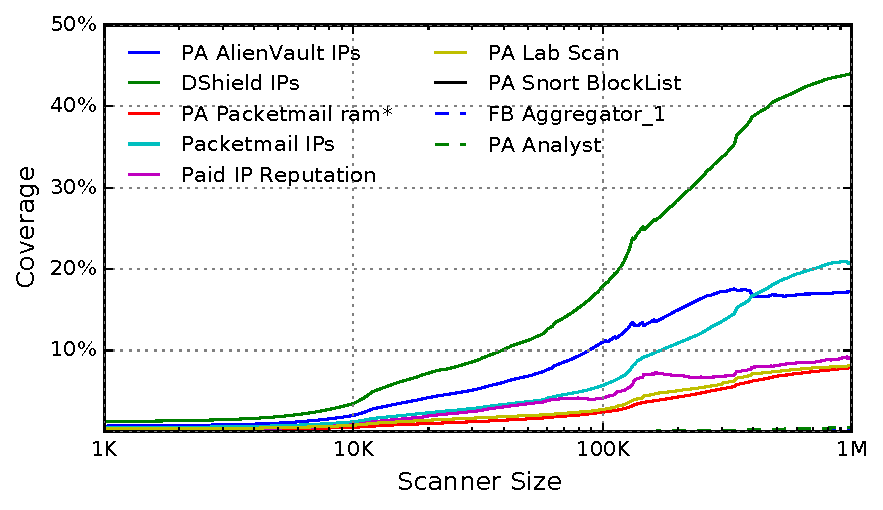
\includegraphics[width=0.8\textwidth]{data_character/images/caida_coverage_cdf.pdf}
\caption{The coverage of each feed on different sizes of scanners.}
\label{fig:caida_coverage_cdf}
\end{figure}

\finding\
The union of all the scan IPs in the feeds covers less than
2\% of the scanners collected by the telescope. Even if we only look
at the scanners with sizes larger than 10,000, the overall coverage is still
around 10\%, suggesting the coverage capability of scan feeds
is very limited. The graph shows that, as the scanner size increases, the coverage of
each feed over the datasets also increases, and large feeds cover more percent
of telescope scanners than small feeds. This trend aligns with the intuition that
scan feeds tend to capture more extensive scanners.

It is surprising that the small scan feeds in our collection have a smaller percentage of their
IPs shared with telescope scanners. This contradicts the idea that small feeds
would contain a larger percentage of extensive scanners (that would most likely also be observed by the telescope).

%Using another metric, the volume of scanners in the
%telescope is over 20 times larger than that of the scan feeds, yet the
%telescope scanners only cover 25.9\% of all of the scanning feeds'
%data. The overall volume of scanning activities is so extensive that
%even a /8 telescope will miss many of them, particularly if scanners
%are selective in targets (avoiding or focusing on certain IP ranges)
%or rate limits (falling below scanner labeling thresholds). The
%coverage curve based on scanner sizes showed that scan feeds are
%better at capturing large scanners, which is intuitive, but that a
%larger feed does not necessarily mean better coverage.


%\begin{table}
%\small
%\caption{Intersection between scan feeds and telescope scanners.
%\textit{Volume} contains the total amount of IPs in each feed from
%Jan. 2016 to July 2016. \textit{Intersection} is the proportion
%of each feed's IPs that overlap with the telescope data.}
%\centering
% \resizebox{0.7\linewidth}{!}{
%\begin{tabular}{l r r }
%\toprule
%Feed & Volume & Intersection \\
%\midrule
%{PA Snort BlockList}     & 312,533   & 18.2\% \\
%{\feedetiprep}           & 293,484   & 22.1\% \\
%{\feedpacketmail}        & 50,723    & 83.6\% \\
%{PA Packetmail ramnode}  & 11,452    & 76.1\% \\
%{\feedalienvault}        & 8,695     & 35.1\% \\
%{PA Malicious IPs}       & 7,960     & 63.3\% \\
%{PA Packetmail CARISIT}  & 5,955     & 71.5\%\\
%{PA SANS Top IPs}        & 3,087     & 77.4\%\\
%{PA Analyst}             & 444       & 52.0\%\\
%{PA Shockpot IPs}        & 156       & 50.0\%\\
%{PA SANS IPs}            & 129       & 63.6\%\\
%{FB Aggregator}          & 103       & 37.9\%\\
%\midrule
%Total & 675,243 & 25.9\%\\
%\bottomrule
%\end{tabular}
%}
%\label{tab:caida_ip_overlap}
%\end{table}




%\subsection{Inter-Category}
%
\textcolor{red}{TODO: Inter category analysis}

%Pick three or four categories of feeds, analyze their \textit{overlap}, \textit{uniquness} and \textit{time attributes}
%\label{sec:analysis}
%\input{content/analysis_scan.tex}

\section{File Hash Threat Intelligence}
\label{sec:hash-analysis}

File hashes in a threat intelligence feed are indicators for malicious
files. It is one of the most lightweight ways to mark files as
suspicious. One can incorporate this data to block malicious
downloads, malicious email attachments, and malware. Likewise, file
hashes can be used to whitelist applications and these feeds can be
used to ensure malicious files do not appear in a customer's
whitelist. In this section we present our analysis on
eight file hash feeds, also collected from December 1st, 2017
to July 20th, 2018. We use the same metrics defined in
Section~\ref{sec:metrics}.

The file hash feeds we collected use a range of different hash
functions to specify malicious files, including MD5, SHA1, SHA256 and
SHA512 (and some feeds provided values for multiple different hash
functions to support interoperability).  Since most indicators in our
dataset are MD5s, we have normalized to this representation by using other
feeds and the VirusTotal service to identify hash aliases for known
malicious files (i.e., which MD5 corresponds to a particualr SHA256
value).  


\begin{table*}[htt]
\footnotesize \tabcolsep=0.11cm
\caption{File hash feeds overview.
The second column group presents feed volume, average daily rate, the number of converted MD5s (Section~\ref{sec:hash-overlap}) and exclusive proportion.
\textit{Not in VT} is fraction of hashes that are not found in VirusTotal, \textit{Not det.} the fraction of hashes that are found in VirusTotal but are not labeled as malicious by any products, and \textit{Detected} the fraction that are found in VirusTotal and are labeled malicious by at least one product. Column \textit{Not in SD} shows the fraction of hashes in a feed that are not in Shadowserver Bin Check. \textit{In NSRL} and \textit{In AppInfo} show the absolute number of hashes found in Shadowserver (Section~\ref{sec:hash-accuracy}). \textit{Exclusive} is based on the MD5-normalized hashes counted under \textit{Converted}. All the other percentages in the table are based on \textit{Volume}.
}
\centering
\small
\begin{tabular}{l | r r r r| r r r | r r r }
\toprule
 Feed         &   Volume  &  Avg. Rate  & Converted &   Exclusive  &   Not in VT    &  Not det.  &   Detected   &   Not in SD &   In NSRL   &  In AppInfo  \\
\midrule
 FB Malware              &    944,257  &  4,070    & 944,257   &    >99.99\%    &     37.41\%    &    50.50\%      &     12.09\%          &    99.89\% &     442 &             706 \\
 PA Malware Indicators   &    39,702   &  171      & 39,702    &     98.73\%    &      0.02\%    &     0.04\%      &     99.94\%          &   >99.99\% &       2 &             0  \\
 PA Analyst              &    38,586   &  166      & 37,665    &     97.97\%    &      4.26\%    &     2.82\%      &     92.92\%          &    99.95\% &       8 &             19 \\
 PA Twitter Emotet       &    1,031    &  4.44     & 960       &     77.29\%    &     11.74\%    &     0.78\%      &     87.49\%          &    99.81\% &       0 &             2  \\
 PA OSINT                &    829      &  3.57     & 783       &     71.65\%    &     19.06\%    &     0.84\%      &     80.10\%          &    99.88\% &       1 &             0  \\
 PA Sandbox              &    298      &  1.28     & 115       &     95.65\%    &     72.81\%    &     0.34\%      &     26.85\%          &    100\% &         0 &             0  \\
 PA Abuse.ch             &    267      &  1.15     & 3         &       100\%    &     98.88\%    &     0.75\%      &      0.37\%          &    100\% &         0 &             0  \\
 PA Zeus Tracker         &    17       &  0.07     & 17        &       100\%    &     88.24\%    &     5.88\%      &      5.88\%          &    100\% &         0 &             0  \\
\bottomrule
\end{tabular}
\label{tab:md5-volume}
\end{table*}

\subsection{Volume}

File hashes, unlike IP threat data, are not transient---a file does
not change from malicious to benign---and thus a far simpler volume
analysis is appropriate. I report volume as the number of new hashes
that are added to each feed during the measurement period.

As seen in Table~\ref{tab:md5-volume-1}, I examine each feed's volume and
average daily rate. Like IP feeds, file hash feeds also vary dramatically in
volume. The majority of the hashes are concentrated in three feeds: FB Malware,
PA Malware Indicators, and PA Analyst, which also exhibit the highest daily rates.
The other feeds are multiple order of magnitude smaller comparatively.

%Every feed has mostly exclusive content, with the ``lowest'' exclusivity belonging to PA Twitter Emotet and PA OSINT (still 77.6\% and 79.29\%, respectively). All other feeds showcase a >97\% exclusive percentage, demonstrating that most MD5 feeds are distinct from each other.

\subsection{Intersection and Exclusive Contribution}
\label{sec:hash-overlap}

As we mentioned earlier, to conduct intersection and exclusive
analysis of file hash feeds, we need to convert indicators into the
same hash type. Here we convert non-MD5 hashes into MD5s, using either
metadata in the indicator itself (i.e., if it reports values for
multiple hash functions) or by querying the source hash from
VirusTotal~\cite{VirusTotal} which reports the full suite of hashes
for all files in its dataset.  However, for a small fraction of hashes
we are unable to find aliases to conver them to the MD5 representation
and must exclude them from the analysis in this section.  This filtering is
reflected in Table~\ref{tab:md5-volume}, in which the Volume column
represents the number of unique hashes found in each feed and the Converted
column is the subset that we have been able to normalize to a MD5
representation.

\finding\ The intersections between hash feeds are minimal,
even among the feeds that have multiple orders of magnitude differences in size.
Across all feeds, only PA Analyst has relatively high intersections: PA Analyst
shares 27\% of PA OSINT's MD5s and 13\% of PA Twitter Emotet's MD5s. PA Malware
Indicators has a small intersection also with these two feeds. All other
intersections are around or less than 1\%. Consequently, the vast majority of
MD5s are unique to one feed, as recorded in column \textit{Exclusive} in
Table~\ref{tab:md5-volume}. The ``lowest'' exclusivity belongs to PA Twitter
Emotet and PA OSINT (still 77.29\% and 71.65\%, respectively). All other feeds
showcase an over 95\% exclusive percentage, demonstrating that most file hash feeds
are distinct from each other.

Due to the different sources of malware between feeds, a low intersection is to
be expected in some cases. For example, PA Twitter Emotet and PA Zeus Tracker
should have no intersection, since they are tracking different malware strains.
The other, more general feeds could expect some overlap, but mostly exhibit
little to no intersection. Considering the sheer volume of the FB Malware feed,
one might expect it would encapsulate many of the smaller feeds or at least
parts of them. This is not the case, however, as FB Malware has a negligible
intersection with all other feeds.

Due to the lack of intersection among the feeds, we omit the latency analysis
of the hash feeds, as there is simply not enough intersecting data to conclude
which feeds perform better with regards to latency.

%\subsection{Latency}
\label{sec:hash-timing}
\note{We might need to delete this section since the overlapped parts are too small, we can't make an argument about latency}

We use the same relative latency definition to calculate the latency distribution of MD5s in each feed, and the calculation is based on the shared data between feeds. Since MD5s are not transient, we don't need to set a time restriction for this computation. Figure~\ref{fig:md5-latency} shows the latency distribution CDF of the feeds.

\begin{figure}[h]
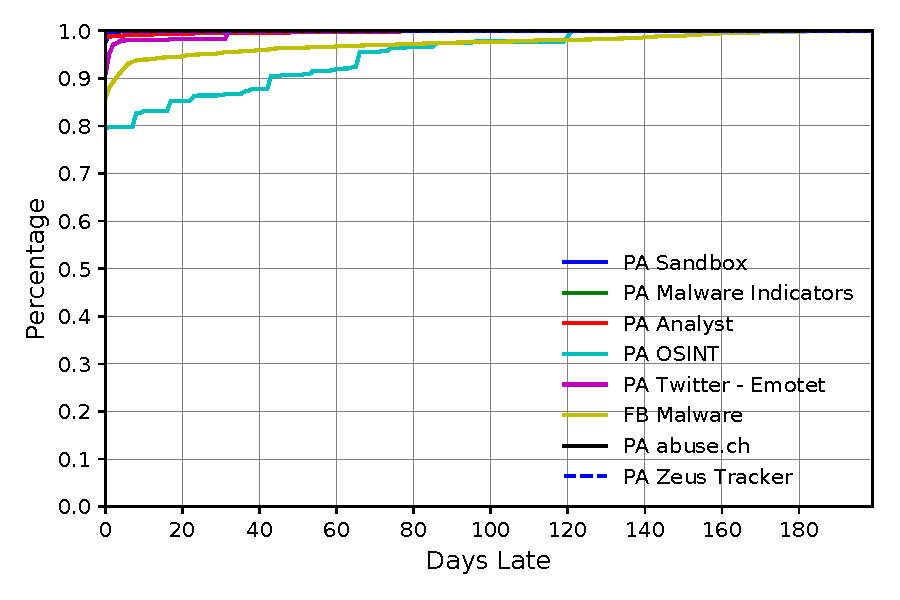
\includegraphics[width=0.9\columnwidth]{images/md5_lateDay.pdf}
\caption{Feed Latency Distribution showing what percentage of each feed's intersected samples are on a particular delay.}
\label{fig:md5-latency}
\end{figure}

As seen in Figure~\ref{fig:md5-latency}, the feeds are roughly grouped into 3 areas. {PA Malware Indicators}, {PA Zeus Tracker}, {PA Analyst}, {PA Twitter - Emotet}, {PA abuse.ch} and {PA Sandbox} report over 90\% of their data first, while {FB Malware }reports over 85\% of its data first. PA OSINT is the outlier in the graph which reports only 80\% of its shared data first. It also has the largest delays, taking almost 50 days to reach 90th percentile and over 70 days to reach 95th percentile.

\finding\ The latency analysis shows which feed is more effective from a timing standpoint, and again demonstrates the fact that a large \ti\ source is not always the quickest at reporting threats.

\subsection{Accuracy}
\label{sec:hash-accuracy}
Assessing the accuracy of file hash feeds presents a problem: there is no
universal ground truth to determine if a file is malicious or benign. Thus,
to gauge the accuracy of the feeds, we use two metrics: a check for malicious
hashes against VirusTotal, and a check for benign hashes against Shadowserver's
Bin Check service. Note that all the percentages discussed below are based on
the \textit{Volume} of each feed.

\subsubsection{VirusTotal}

VirusTotal is a service that is often used when analyzing
malware to get a base of information about a suspected file.
Anyone can upload a file to be scanned. Upon submission, these files will be
scanned by more than 70 antivirus scanners, which creates a report on how many
antivirus scanners mark it malicious, among other information. In this analysis,
we query VirusTotal for the hashes in each file hash feed and then inspect the
percent of hashes that are marked as malicious and how many AV scanners have
recorded them. Due to the high volume of the FB Malware feed and the query
rate limit of VirusTotal, we randomly sampled 80,000 hashes from the feed for
this analysis.

Table~\ref{tab:md5-volume} shows a breakdown of the base detection rates for
each feed from VirusTotal. As the PA feeds decrease in volume, the rates at
which they are found in VirusTotal also decreases. The larger PA feeds have a
much higher detection rate than their smaller counterparts. On the other hand,
FB Malware only has 37\% of its data detected by antivirus scanners and 50\% in
VirusTotal with no detection despite being the largest feed. This could indicate
that FB Malware focuses on threats that specifically target Facebook and that
are not as relevant to most VirusTotal users, such as malicious browser
extensions~\cite{dekoven2017malicious, jagpal2015trends, kapravelos2014hulk}.
This might undermine the limited coverage of VirusTotal as an oracle to detect
targeted threats that are not of broader interest.

\begin{figure}[t]
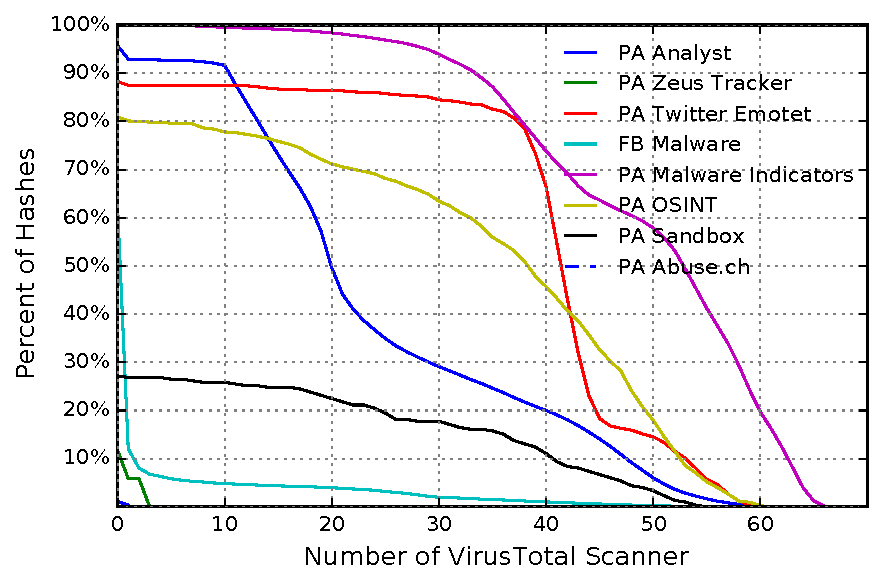
\includegraphics[width=0.95\columnwidth]{images/hash_vt_cdf.pdf}
\caption{VirusTotal detection distribution. Each point means the proportion of indicators (Y value) in a feed that is detected by \textit{over} X number of AV scanners in VirusTotal.}
\label{fig:vt-cdf}
\end{figure}

To further understand how the scanners in VirusTotal report the feed's data,
we plot a graph of what percentage of hashes in each feed are detected by how many
VirusTotal scanners. As seen in Figure~\ref{fig:vt-cdf}, four feeds have more
than 50\% of their samples detected by over 20 scanners. PA Malware Indicators
and PA Twitter Emotet did not experience a large detection drop before 35 scanners,
indicating that most indicators in the two feeds are popular malicious files
recognized by many AV vendors. While PA Sandbox has a large percent of its hashes
not presented in VirusTotal, over 70\% of its samples that are detected are marked
by over 20 AV scanners, showcasing a high confidence detection.

\subsubsection{Shadowserver}

To more fully gauge the accuracy of the file hash feeds,
we also examined how each feed measured against Shadowserver's Bin Check
Service~\cite{shadowserver}. The service checks file hashes against NIST's
National Software Registry List (NSRL) in addition to Shadowserver's own repository of
known software. Table~\ref{tab:md5-volume} details how each feed compares with
Shadowserver's Bin Check service.

It might be expected that there would be no hash found with Shadowserver's Bin
Check service, but it is not the case. Some of the samples from the feeds that
appear in Shadowserver are well known binaries such as versions of Microsoft
Office products, Window's Service Packs, calc.exe, etc. In the event malware
injects itself into a running process, it remains plausible that some of these
well-known binaries find their way into \ti\ feeds from users wrongly attributing
maliciousness. While FB Malware has over one thousand hashes in Shadowserver, this
is not a widespread issue, as all feeds have <1\% of their hashes contained within
Shadowserver's Bin Check service.
%, shown in Table \ref{tab:md5-volume}.
This showcases that while there are a few exceptions, the feeds mostly do not
contain well-known, benign files.

\finding\ Each PA feed has a negligible rate of occurrence within Shadowserver
regardless of their VirusTotal detection, showing they do not contain generic
false positives. Larger feeds exhibit high VirusTotal detection rates except
for FB Malware, while small feeds have relatively low detection rates.
This suggests that small hash feeds might focus more on specific malicious files
that are not widely known.
FB Malware has a low VirusTotal occurrence despite
its size and has over one thousand hashes in Shadowserver, but its overall low
percentage of hashes within Shadowserver indicates that it does not contain
many known files and might have threats not typically recognized by
VirusTotal's scanners.


\section{Longitudinal Comparison}
\label{sec:new_vs_old}

In addition to the measurement period considered so far (December 1, 2017 to July 20, 2018), I also analyzed data from the same IP feeds from January 1, 2016 to August 31, 2016. These two measurement periods, 23 months apart, allow us to measure how these IP feeds have changed in two years. Table~\ref{tab:old-volume-overview-1} and
Table~\ref{tab:old-volume-overview-2} summarizes the differences between these two measurement periods. \colname{Avg. Rate} shows the percentage of daily rate changed over the old feeds.
The two columns under \colname{Unrt} show the unroutable rates of feeds in 2016 and 2018 separately. The two columns under \colname{CDN} present the number of IPs fall in CDN IP ranges in old and new data. In the table, \colname{2018} represents the current measurement period and \colname{2016} the period  January 1, 2016 to August 31, 2016.
\newcolumntype{H}{>{\setbox0=\hbox\bgroup}c<{\egroup}@{}}

\begin{table}[t!]
\centering
\caption{Data changes in IP feeds compared against the ones in 2016, \colname{Avg. Rate} shows the percentage of daily rate changed over the old feeds.
The two columns under \colname{Unrt} show the unroutable rates of feeds in 2016 and 2018 separately. The two columns under \colname{CDN} present the number of IPs fall in CDN IP ranges in old and new data.}
\label{tab:old-volume-overview}
\scriptsize
 \begin{tabular}{l r H H H H H r r r r }
 \toprule
& & & & & & & \multicolumn{2}{c}{\colname{Unroutable}} & \multicolumn{2}{c}{\colname{CDN}} \\
\cmidrule(lr){8-9}\cmidrule(l){10-11}
 \colname{Feed} & \colname{Avg. Rate} & \colname{Exclusive} & \colname{Unrt} & \colname{Unrt} & \colname{CDNs} & \colname{New} &   2016 &  2018 &  2016  &  2018 \\ %& \colname{Unrt} \\
  \midrule
  \textbf{Scan Feeds} \\
  %\cline{1-1}
  PA AlienVault IPs 	    & $+$1,347\%    & 63.3\%  	& 18218.0  & +0.0        & +0     & 100\%   & 0.0\%    & 0.0\%      & 0    & 0 \\
  PA Packetmail ram* 	    & $+$733\%   & 75.3\% 	 	& 6749.8   & +0.0        & +0     & 100\%   & <0.01\%    & <0.01\%  	& 0    & 0 \\
  Packetmail IPs 	        & $+$135\%   & 83.4\% 	 	& 11145.8  & +0.0        & +0     & 99.4\%  & 0.0\%    & 0.0\%    	& 0     & 0\\
  Paid IP Reputation 	    & $-$57\%   & 97.7\% 	 	& 59430.9  & -7.08       & -889   & 91.3\%  & 8.73\%    & 1.65\%  & 910     & 21\\
  PA Lab Scan 	            & $-$1\%    & 85.1\% 	 	& 5921.8   & +<0.01      & +0     & 99.8\%  & 0.0\%     & <0.01\%   & 0   & 0 \\
  PA Snort BlockList 	    & $-$97\%   & 99.4\% 	 	& 123093.3 & +0.41       & -1     & 86.6\%  & <0.01\%     & 0.42\% 	& 1     & 0\\
  FB Aggregator$_1$ 	    & $+$332\%   & 83.8\% 	 	& 617.3    & +0.0        & -6     & 100\%   & 0.0\%     & 0.0\%     & 6   & 0 \\
  PA Analyst 	            & $-$44\%   & 52.5\% 	 	& 137.2    & +0.41       & +0     & >99.9\% & 0.0\%  	& 0.41\%    & 0   & 0\\

  %\midrule
  \textbf{Botnet Feeds} \\
  %\cline{1-1}
  PA CI Army 	            & $+$114\%   & 96.8\% 	& 4996.6  & +0.0     & +0    & 100\%  & <0.01\%  & <0.01\% & 0    & 0\\
  Paid IP Reputation 	    & $-$39\%   & 99.8\% 	& 17249.7 & +1.02    & +59   & 80.5\% & 0.63\%   & 1.66\%  & 15    & 74\\
  PA Botscout IPs 	        & $+$1\%    & 74.5\% 	& 5762.6  & +0.08    & -1    & 100\% & 0.01\%    & 0.09\%  & 1     & 0\\
  PA VoIP Blacklist 	    & $+$252\%   & 89.7\% 	& 732.4   & +0.32  	 & +0    & 100\% & 0.0\%     & 0.32\%  & 0    & 0\\
  PA Compromised IPs 	    & $-$36\%   & 94.9\% 	& 1515.8  & -0.10 	 & +0    & 100\% & 0.10\%    & 0.0\%   & 0   & 0\\
  PA Blocklist Bots 	    & $-$95\%	  & 82.0\% 	& 8282.6  & +0.0     & +0    & 100\% & 0.0\%     & 0.0\%   & 0    & 0 \\
  PA Project Honeypot 	    & $+$63\%	  & 48.3\% 	& 260.2   & +0.0     & +0    & 100\% & 0.0\%     & 0.0\%   & 0    & 0 \\

  %\midrule
  \textbf{Brute-force Feeds} \\
  %\cline{1-1}
   Badips SSH 	             & $+$30\%   & 94.2\% 	& 45479.9   & +0.12    & +1     & 97.6\% & 0.07\%      & 0.19\% & 0   & 1    \\
   Badips Badbots 	         & $+$1,732\%    & 87.6\%     & 1085.5    & +1.04    & +1064  & 92.6\% & 0.0\%      & 1.04\%  & 187 & 1,251   \\
   Paid IP Reputation 	     & $-$62\%   & 91.0\% 	& 19483.5   & -6.52    & -325   & 98.4\% & 6.55\%    & 0.03\%   & 335 & 10  \\
   PA Brute-Force 	         & $-$72\%   & 97.3\% 	& 63016.8   & +0.0     & +0     & 100\%  & 0.0\%      & 0.0\%   & 0   & 0  \\
   Badips Username*          & $+$3,040\%    & 16.6\% 	& 175.7     & +0.53    & +0     & 95.7\% & 0.0\%     & 0.53\% 	& 0  & 0\\
   Haley SSH 	             & $+$428\%   & 13.6\% 	& 226.6     & -0.01    & +0     & 94.8\% & 0.04\% 	& 0.03\%    & 0  & 0\\
   FB Aggregator$_2$ 	     & $+$387\%   & 42.4\% 	& 358.3     & -0.12    & +0     & 100\%  & 0.12\% 	& 0.0\%     & 0  & 0\\
   Nothink SSH 	             & $+$886\%   & 53.8\% 	& 778.5     & 0.95     & +0     & 86.4\% & 0.56\%	& 1.51\%    & 0  & 0\\
   Dangerrulez Brute 	     & $+$0\%	   & 9.15\% 	& 1109.8    & +0.0     & -1     & 99.8\% & 0.0\%    & 0.0\% 	& 1  & 0 \\

  %\midrule
  \textbf{Malware Feeds} \\
  %\cline{1-1}
  Paid IP Reputation 	       & $-$36\%	 & 96.2\% 	& 35273.7 	& -0.05     & -11,776   & 94.3\%& 0.18\%   & 0.13\% & 15265     & 3,489\\
  FB Malicious IPs 	           & $-$77\%   & 99.6\% 	& 17649.6   & -4.4      & -264      & 99.9\% & 6.81\%  & 2.14\% & 264     & 0   \\
  Feodo IP Blacklist 	       & $+$0\%    & 24.6\% 	& 589.0     & +0.0      & +0	    & 52.4\% & 0.0\%   & 0.0\% 	& 0      & 0 \\
  Malc0de IP Blacklist 	       & $-$9\%    & 60.0\%   & 143.1     & +0.0   	& -121      & 99.2\% & 0.0\%   & 0.0\%  & 132    & 11\\
  PA Bambenek C2 IPs 	       & $+$79\%   & 74.3\% 	& 72.9      & +9.13     & +0	    & 100\%  & 0.0\%   & 9.13\% & 0     & 0 \\
  PA SSL Malware IPs 	       & $-$34\%   & 30.1\% 	& 73.0      & +0.0      & +0	    & 100\%  & 0.0\%   & 0.0\%  & 0   & 0 \\
  PA Analyst 	               & $-$93\%    & 76.4\% 	& 917.7     & +0.0      & +0        & 99.8\% & 0.34\%  & 0.0\%  & 0  & 0\\
  PA Abuse.ch* 	               & $-$99\%   & 2.19\% 	& 4755.2    & +2.63     & +0        & 44.9\% & 0.49\%  & 3.12\% & 0  & 0\\
  PA Mal-Traffic-Anal  	       & $-$53\%   & 39.0\% 	& 25.7      & +0.51     & +0        & 100\%  & 0.0\%   & 0.51\%  & 0    & 0 \\
  Zeus IP Blacklist 	       & $-$66\%   & 24.3\%   & 164.8     & +0.0      & -6        & 49.2\% & 0.0\%   & 0.0\%   & 6  & 0\\


  %\midrule
  \textbf{Exploit Feeds} \\

Badips HTTP    & $+$326\%    & 98.0\% 	& 11693.1 	& +0.37  & +2,154  & 97.8\%   & 0.30\%  & 0.67\%  & 436 & 2,590 \\
Badips FTP 	   & $+$556\%    & 98.1\% 	& 6132.7    & +1.32  & +2      & 82.7\%   & 0.01\%  & 1.33\%  & 0   & 2\\
Badips DNS 	   & $+$9,525\%     & 96.9\% 	& 51.8      & +0.33  & +237    & 98.8\%   & 0.17\%  & 0.50\%  & 7   & 244  \\
Badips RFI 	   & $+$226\%    & 29.1\%  & 40.9      & +2.22  & -1      & 67.6\%   & 0.0\%   & 2.22\%  & 0   & 0  \\
%Badips SQL 	   & 66.6\% 	& 0.0 	& 0.0 \\

 \textbf{Spam Feeds} \\
  %\cline{1-1}
Paid IP Reputation 	 & $+$133\%	     & 99.9\%      & 4626.5    & +19.4   & +0      & 89.7\%  & 59.3\%    & 78.7\% & 0   & 0\\
Badips Spam 	     & $+$12,767\%    & 40.0\%      & 320.5     & +0.02   & +0      & 99.0\% 	& 0.0\%     & 0.02\% & 0   & 0 \\
Badips Postfix 	     & $-$53\%       & 99.1\%      & 52594.8   & +1.28   & +1      & 96.6\%  & <0.01\%   & 1.29\% & 0   & 1\\
PA Botscout IPs 	 & $+$18\%	     & 97.5\% 	  & 4337.3    & +0.06   & +0      & >99.9\%	& 0.0\%     & 0.06\% & 0   & 0 \\
AlienVault IP Rep 	 & $+$8\%	    & 87.2\% 	  & 1497.7    & -0.50   & +561    & 98.8\% 	& 0.57\%	& 0.07\% & 479  & 1,040 \\


\bottomrule
\end{tabular}
\end{table}



%\caption{Data changes in IP feeds compared against the ones in 2016, \colname{Avg. Rate} shows the change percentage of daily rate.
%For small changes we use ``\%'', for large changes we use ``x'', indicating x times.
%\colname{Unrt} shows the changes between unroutable rate with before. \colname{CDNs} are the changes on the number of IPs fail in into the CDN IP ranges.
%\colname{New} shows the percentage of indicators that are new to the recent feed compared with the old feed.}


\textbf{Volume.}
As shown in Table~\ref{tab:old-volume-overview-1} and ~\ref{tab:old-volume-overview-2}, feed volume has definitely changed after two years. Among 43 IP feeds that overlap both time periods,
21 have a higher daily rate compared with 2 years ago, 15 feeds
have a lower rate, and 7 feeds do not change substantially (the difference is below 20\%).
Volume can change dramatically over time, such as {\feedTSAlienVault}
in the scan category which is 13 times larger than before. On the other hand, a feed like {\feedTSBots} is now over 90\% smaller.

\textbf{Intersection and Exclusive Contribution.}
Despite the volume differences, the intersection statistics between feeds are largely the same across two years,
with feeds in scan and brute-force having high pairwise intersections and
feeds in other categories being mostly unique. Certain specific pairwise relations also did not change.
For example, {\feedbadipssh} still shared over 90\% of data in {\feeddangerrule} back in 2016, and {\feedetiprep} in malware
was still the only feed that has a non-trivial intersection with multiple small feeds.
Again, most data was exclusive to each feed two years ago: Across all
six categories more than 90\% of the indicators are not shared between feeds.

\textbf{Latency.}
The latency relationship between feeds was also similar:
timely feeds today were also timely two years ago, and the same with tardy feeds.
%The latency difference between feeds are bigger then compared with data, but small feeds
%still report a significant portion of their shared data.

\textbf{Accuracy.}
Feeds have more unroutable IPs now than before as shown in Table~\ref{tab:old-volume-overview-1} and~\ref{tab:old-volume-overview-2}:
In 2016, 22 of the 43 IP feeds had at least 1 unroutable IP; four feeds had unroutable rates over 1\%.
When checking the intersection with popular CDNs,
the feeds that contain IPs in CDN ranges two years ago are also the ones that have these IPs today.

\textbf{Shared indicators 2016--2018.}
I compared the data I collected from each feed in the two time periods, and found that 30
out of 43 feeds in 2018 intersect with their data from two years ago, and 9 feeds have
an intersection rate over 10\%. Three feeds in malware category, namely {\feedfeodo},
{\feedTSAbusech} and {\feedzeus}, have over 40\% of their data shared with the past feed,
meaning a large percent of C\&C indicators two years ago are still
identified by the feeds as threats today. Feeds in the botnet category, however, are very distinct from the
past, with all feeds having no intersection with the past except {\feedetiprep}.
\section{Absolute Latency}
\label{sec:abs_latency}

I defined the latency metric in this chapter as relative latency between \ti\
sources, since it is easy to compute and allows consumers to compare feeds
to each other on this aspect. However, it is also critical to know
about the absolute latency distribution of indicators. Absolute latency
represents how fast a feed can actually report a threat, which directly decides
the effectiveness of the data when used in a pro-active way. As I already
discussed in Section~\ref{sec:ip-timing}, absolute latency is hard to measure,
as I do not have ground truth of the underlying threat.

In Section~\ref{sec:completeness}, I used an Internet telescope as the approximation
for ground truth to measure the coverage of scan feeds. In Section~\ref{sec:hash-accuracy},
I used VirusTotal as an oracle to measure the accuracy of file hash feeds.
Although these sources are not real ground truth and it is unclear how far away
they are, these large and well-managed sources can help us, to a certain extent,
profile the performance of \ti\ feeds. In this section, I use these two sources
again to approximate the absolute latency of indicators in scan IP feeds and
malicious file hash feeds.

More specifically, I measure the latency of IPs in scan feeds
relative to the first occurrence time of the same IP in the scanners collected from
the telescope. Considering the massive size of the telescope, it should presumably
detect scanners much sooner after the scanning event actually happened.
I measure latency of file hashes relative to the \texttt{first\_seen} timestamps queried
from VirusTotal. The \texttt{first\_seen} timestamp represents the time when the corresponding
file is first uploaded to VirusTotal. VirusTotal is a very popular service and it is a
convention for many security experts to upload new malware samples to VirusTotal once
they discovered them. Therefore, this timestamp roughly entails when the security
community first noticed the malicious file and can be a good approximation for absolute
latency.

\begin{figure}[t!]
\centering
\subfloat[Latency distribution in scan feeds relative to the Internet telescope]{
	\label{fig:scan_abs_firstseen}
	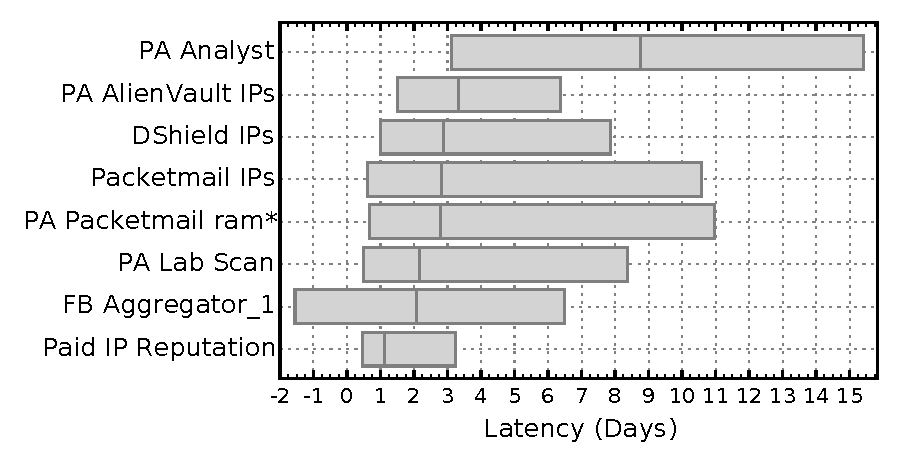
\includegraphics[width=0.8\textwidth]{data_character/images/scan_abs_latency.pdf}}

\subfloat[Latency distribution in file hash feeds relative to VirusTotal]{
	\label{fig:hash_abs_firstseen}
	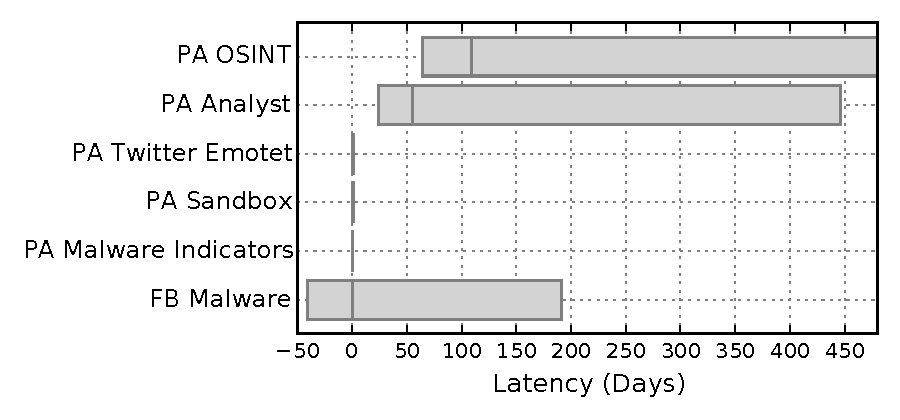
\includegraphics[width=0.8\textwidth]{data_character/images/hash_abs_latency.pdf}}

\caption{Distribution of indicators' latency in scan and file hash feeds.
The scan feeds' distribution are calculated in hour granularity while
the file hash feeds' distribution are calculated in day granularity.}
\label{fig:abs_firstseen}
\end{figure}


Figure~\ref{fig:abs_firstseen} show the latency distribution of each feed, using
the same plotting convention as in Section~\ref{sec:ip-timing}. Some feeds are not
shown in the figure as there are too little data points in those feeds to reason
about distribution.

\finding\
Comparing Figure~\ref{fig:scan_abs_firstseen} to Figure~\ref{fig:scan_firstseen},
I can see that the median latency of feeds are all larger. This is consistent with
my assumption that a large sensor tends to receive indiscriminate scanners sooner.
Scan feeds' median lantecy are one to three days relative to the Internet telescope,
except {\feedTSAnalyst}, whose median latency is almost nine days.
The order of median latency between feeds changed compared with Figure~\ref{fig:scan_firstseen},
but since the original relative median latencies among scan feeds are very close,
the new order here is more likely to be statistics variances. Also, note that
although the {\feedTSAlienVault} seems much slower than it is in
Figure~\ref{fig:scan_firstseen}, its 75 percentile latency is still the second
smallest one.

On the other hand, the latency distributions of hash feeds vary more dramatically.
PA Malware Indicators, PA Sandbox and PA Twitter Emotet are almost as fast as
VirusTotal: all three feeds have 25 percentile and median latency equal to zero.
PA OSINT and PA Analyst are comparatively much slower, and PA OSINT even has a 75
percentile latency of 1680 days. This might be because of the heterogeneous nature of
malware feeds. The figure also shows that feed volumes do not imply
their latency, as PA Analyst and FB Malware are much slower than the small hash
feeds.

Figure~\ref{fig:abs_firstseen} demonstrates that the Internet telescope and VirusTotal
are indeed good approximations for absolute latency measurement, as most
indicators in \ti\ feeds are observed relatively later. However, every scan
feed has over 2\% of its indicators detected earlier than the telescope did.
{\feedFBBasecamp} and {\feeddshield} even have over 10\% of their indicators observed
earlier. There is also a similar case in file hash feeds. This aligns with
my observation in Section~\ref{sec:ip-timing} that small feeds can still report
a non-trivial amount of their data first. Another interesting observation is that
both Facebook feeds, {\feedFBBasecamp} and FB Malware, have a large percent of
their data observed earlier than the telescope or VirusTotal. This again suggests
that Facebook (and its threat intelligence partners) might face more targeted
threats, so those threats will be first observed by Facebook.

\section{Discussion}
\label{sec:discussion}

\subsection{Metrics Usage}
Threat intelligence has many different potential uses. For example,
analysts may consume threat data interactively during manual
incident investigations, or may use it to automate the detection of
suspicious activity and/or blacklisting.  When not itself
determinative, such information may also be used to \emph{enrich}
other data sources, informing investigations or aiding in automatic
algorithmic interventions. We have introduced a set of basic threat
intelligence metrics---volume, intersection, unique contribution,
latency, coverage and accuracy---that can inform and quantify each of
those uses.  Depending on a number of factors, such as the intended
use case and the cost of false positives and negatives, some of
these metrics will become more or less important when evaluating a
\ti\ source. For example, a feed with poor accuracy but
high coverage might be ideal when an analyst is using a \ti\ source
interactively during manually incident investigations (since in this
case, the analyst, as a domain expert, can provide additional filtering
of false positives). Similarly, latency might not be a critical metric
in a retrospective use case (e.g., post-discovery breach
investigation).  However, if an organization is looking for a
\ti\ source where the IPs are intended to be added to a firewall's
blacklist then accuracy and latency should likely be weighted over
coverage, assuming that blocking benign activity is more costly.

Another common real-world scenario is that a company has a limited
budget to purchase \ti\ sources and has a specific set of threats (\ie
botnet, brute-force) they are focused on mitigating. In such cases,
the metrics we have described can be used directly in evaluating \ti\
options, biasing twoards sources that maximize coverage of the most
relevant threats while limiting intersection.


\subsection{Data Labeling}
Threat intelligence IP data carries different meanings. To properly use this
data, it is critical to know what the indicators actually mean: whether
they are Internet scanners, members of a botnet or malicious actors who
had attacked other places before. We have attempted to group feeds by their
intended meaning in our analysis.

However, this category information, which primarily comes from \ti\ sources
themselves, is not always available. Feeds such as {\feedalienvault} and
Facebook Threat Exchange sources contain a significant number
of indicators labeled ``Malicious'' or ``Suspicious.'' The meanings of
these indicators are unclear, making it difficult for consumers to decide
how to use the data and the possible consequences.

For feeds that provide category information, it is sometimes too broad
to be meaningful. For example, multiple feeds in our collection
simply label their indicators as ``Scanner.'' Network scanning can
represent port scanning (by sending SYN packets), or a vulnerability scan (by
probing host for known vulnerabilities). The ambiguity here, as a result of
ad-hoc data labeling, again poses challenges for security experts when using
\ti\ data.

Recently, standard \ti\ formats have been proposed and developed, notably
IODEF~\cite{IODEF}, CybOX~\cite{CybOX} and STIX~\cite{STIX}, that try to
standardize the threat intelligence presentation and sharing. But these
standards focus largely on the data format. There is room
to improve these standards by designing a standard \emph{semantics} for threat
intelligence data.

%Even if we just use it to block traffic, it is very difficult to justify the
%performance of this feed, let alone to use it during a threat forensic analysis.

% wrong categorization.
%Sometimes the categorization provided by the provider might not be acurrate. For example, the
%\feedTSSnort\ is labelled as scanners by the PA, however, we found little intersection between
%this source and other scan sources, also little intersectio with the scanners collected
%by the Internet telescope. We suspect the data provided by this feed is not real Internet scanners.

\subsection{Limitations}
There are several questions that our study does not address. We attempted to collect data from a diverse set of
sources, including public feeds, commercial feeds and industrial exchange feeds,
but it is inherently not comprehensive. There are some prohibitively expensive or
publication-restricted data sources that are not available to us. More specialized measurement
work should be done in the future to further analyze the performance of these
expensive and exclusive data sources.

%Future work might be to obtain access to a larger more diverse set of \ti\
%sources or incentives \ti\ providers to allow a neutral third-party to
%replicate our metrics.

A second limitation is our visibility into how different companies use threat
intelligence operationally. For a company, perhaps the most useful kind of metric
measures how a threat intelligence source affects its main performance indicators
as well as its exposure to risk. Such metrics would require a deep integration
into security workflows at enterprises to measure the operation effect of decisions
made using threat intelligence. This would allow CIOs and CSOs to better understand
exactly what a particular threat intelligence product contributes to a company. As
researchers, we do not use \ti\ operationally. A better understanding of operational
needs would help refine our metrics to maximize their utility for operations-driven consumers.

The third limitation is the lack of ground truth, a limitation shared
by all the similar measurement work. It is simply very difficult to obtain the full picture
of a certain category of threat, making it very challenging to precisely determine accuracy and coverage of feeds. In this
study, we used data from an Internet telescope and VirusTotal as a close approximation.
There are also a handful of cases where a security incident has been comprehensively studied by
researchers, such as the Mirai study~\cite{antonakakis2017understanding}, and such efforts
can be used to evaluate certain types of \ti\ data. But such studies are few in number.
One alternative is to try to establish the ground truth for a specific network.
For example, a company can record all the network traffic going in and out of its own network,
and identify security incidents either through its IDS system or manual forensic analysis.
Then it can evaluate the accuracy and coverage of a \ti\ feed under the context of its
own network. This can provide a customized view of \ti\ feeds.


%Our metrics can be used as a starting point and refined as needed based on an
%improved understanding of how \ti\ is currently used operationally and metrics
%that might improve the quality of \ti\ so that it could be used for additional tasks.


%%
%% Below are comments
%%
\begin{comment}
\subsection{Independence between Metrics}
We evaluated a large range of \ti\ sources using six metrics, it is
interesting to see if there is any correlation between these metrics.
We already compared the relation of between volume and latency of IP feeds
in Section~\ref{sec:ip-timing} and showed that there is not a strong correlation. Similar cases
can also be observed, for example, between volume and accuracy that neither high or low
volume implies high accuracy in our feeds collection. Also, both IP and MD5 feeds show
that the exclusive rate is irrelevant with the feeds' size.

To formally address this question, we check the correlation coefficient between
\emph{Volume}, \emph{Exclusive Contribution}, \emph{Latency} and \emph{Accuracy}
in IP and MD5 feeds(when available). The result shows a low(below 0.5) correlation across all comparison.
This means when choosing between different \ti\ sources, we need to evaluate them comprehensively
on multiple perspectives, as different perspective does not imply each other.

Coverage correlate with volume in our scan feeds, which is not a surprise since volume naturally
implies coverage when the accuracy are close.


\subsection{Limited Coverage}
Most \ti\ indicators are exclusive to each feed, for both IP and MD5 sources.
Moreover, when comparing with broad sensor data in known categories like Internet scanning,
fewer than 2\% of ``known bad'' addresses appear in all the data sources we
analyzed. These suggest several non-exclusive possibilities. First is that the
underlying space of indicators (both IP addresses and malicious file hashes) is
large and each individual data sources can at best sample a small fraction
thereof. Second, different measurement methodologies---even for the same threat
category---will select for different sub distributions of the
underlying ``ground truth'' data.  Third, this last effect is likely
exacerbated by the fact that not all threats are experienced uniformly
across the Internet and thus, some kinds of methodologies, will skew
to either favor or disfavor targeted attacks.

This implies that \ti\ consumers should focus more on how the feeds related to the
specific threat that the consumers are mostly exposed to, instead of blindly trying to maximize
coverage or to find the ``best'' feed. Future work would be to correlate \ti\ feeds' data
with the companies or organizations' network traffic and evaluate feeds under specific environments.
\end{comment}

\section{Related Work}
\label{sec:background}

Several studies have examined the effectiveness of blacklist-based threat
intelligence~\cite{kuhrer2014paint, ramachandran2006revealing, ramachandran2007filtering, sheng2009empirical, sinha2008shades}.
Ramachandran~\etal~\cite{ramachandran2007filtering} showed that spam blacklists
are both incomplete (missing 35\% of the source IPs of spam emails captured in
two spam traps), and slow in responding (20\% of the spammers remain unlisted
after 30 days). Sinha~\etal~\cite{sinha2008shades} further confirmed this
result by showing that four major spam blacklists have very high false negative
rates, and analyzed the possible causes of the low coverage.
Sheng~\etal~\cite{sheng2009empirical} studied the effectiveness of
phishing blacklists, showing the lists are slow in reacting to
highly transient phishing campaigns. These studies focused on specific
types of threat intelligence sources, and only evaluated their operational
performance rather than producing empirical evaluation metrics for
threat intelligence data sources.

Other studies have analyzed the general attributes of threat
intelligence data.  Pitsillidis~\etal~\cite{tasters:imc12} studied the
characteristics of spam domain feeds, showing different perspectives
of spam feeds, and demonstrated that different feeds are suitable for
answering different questions.  Thomas~\etal~\cite{thomas2016abuse}
constructed their own threat intelligence by aggregating the abuse
traffic received from six Google services, showing a lack of
intersection and correlation among these different sources.  While
focusing on broader threat intelligence uses, these studies did not
focus on generalizable threat metrics that can be extended beyond the work.

Little work exists that defines a general measurement methodology to
examine threat intelligence across a broad set of types and categories.
Metcalf~\etal~\cite{metcalf2015blacklist} collected and measured IP
and domain blacklists from multiple sources, but only focused on volume
and intersection analysis. In contrast, we formally define a set of threat intelligence
metrics and conduct a broad and comprehensive study over a rich variety of
threat intelligence data. We conducted our measurement from the
perspective of consumers of \ti\ data
to offer guidance on choosing between different sources.
Our study also demonstrated the limitation of threat intelligence more thoroughly,
providing comprehensive characteristics of cyber threat intelligence that no work had
addressed previously.

\section{Conclusion}
\label{sec:conclusion}

This paper has focused on the simplest, yet fundamental, metrics about
threat intelligence data. Using the proposed metrics, we measured a broad
set of \ti\ sources, and reported the characteristics and limitations of
\ti\ data. In addition to the individual findings mentioned in each section, here
we highlight the high-level lessons we learned from our study:

%---effectively investigating the extent to which disparate
%sources are measuring the same underlying empirical phenomena and can
%be meaningfully used to directly anticipate future attacks.  Thus far
%the evidence for this goal is spartan at best.

\begin{itemize}
	\item \ti\ feeds, far from containing
    homogeneous samples of some underlying truth, vary tremendously in the
    kinds of data they capture based on the particularities of their
    collection approach. Unfortunately, few \ti\ vendors explain the
    mechanism and methodology by which their data are collected and thus
    \ti\ consumers must make do with simple labels such as
    ``scan'' or ``botnet'', coupled with inferences about the
    likely mode of collection. Worse, a significant amount of data does not
    even have a clear definition of category, and is only labelled as
    ``malicious'' or ``suspicious'', leaving the ambiguity to consumers to
    decide what action should be taken based on the data.

    \item There is little evidence
    that larger feeds contain better data, or even that there are
    crisp quality distinctions between feeds across different categories
    or metrics (i.e., that a \ti\ provider whose feed performs well on one
    metric will perform well on another, or that these rankings will hold
    across threat categories). How data is collected also does not
    necessarily imply the feeds' attributes. For example, crowdsourcing-based feeds (\eg\ Badips feeds), are not always slower in reporting data
    than the self-collecting feeds (like \feedetiprep).

    \item Most IP-based \ti\ data sources are collections of
    singletons (i.e., that each IP address appears in at most one source)
    and even the higher-correlating data sources frequently have
    intersection rates of only 10\%. Moreover, when comparing with broad
    sensor data in known categories with broad effect (e.g., random
    scanning) fewer than 2\% of observed scanner addresses appear in most of
    the data sources we analyzed; indeed, even when focused on the largest
    and most prolific scanners, coverage is still limited to 10\%. There
    are similar results for file hash-based sources with little overlap
    among them.
\end{itemize}

The low intersection and coverage of \ti\ feeds could be the result of
%Taken together these suggest
several non-exclusive possibilities.
First is that the underlying space of indicators (both IP addresses
and malicious file hashes) is large and each individual data source
can at best sample a small fraction thereof.  It is almost certain
that this is true to some extent.  Second, different collection
methodologies---even for the same threat category---will select for
different sub distributions of the underlying ground truth data.
Third, this last effect is likely exacerbated by the fact that not all
threats are experienced uniformly across the Internet and, thus,
different methodologies will skew to either favor or disfavor targeted
attacks.


\begin{comment}
While resolving this question is of academic interest, it seems clear
that blindly using \ti\ data---even if one could afford to acquire
many such sources---is unlikely to be effective.  Proactive defenses,
such as blocking network connections or file executions that match
\ti\ indicators, are predicated on knowing, in advance, a large
fraction of the universe of future indicators; the evidence is that
this is not currently possible.  While there may be some utility in
doing this even for the small percentage of malicious traffic that may
be identified, this must be balanced against the costs of obtaining
and managing \ti\ data as well as the risks associated with false
positives.
\end{comment}


Based on our experience analyzing \ti\ data, we try to provide several
recommendations for the security community on this topic moving forward:

\begin{itemize}
    \item The threat intelligence community should standardize data labeling,
    with a clear definition of what the data means and how the data is collected. Security experts can then assess
    whether the data fit their need and the type of action should be taken
    on this data.

    \item There are few rules of thumb in selecting among \ti\ feeds,
    as there is not a clear correlation between different feed properties.
    Consumers need empirical metrics, such as those we describe, to
    meaningfully differentiate data sources, and to prioritize certain metrics
    based on their specific need.

    \item Blindly using \ti\ data---even if one could afford to acquire
    many such sources---is unlikely to provide better coverage and is
    also prone to collateral damage caused by false positives. Customers
    need to be always aware of these issues when deciding what action
    should be taken on this data.

    \item Besides focusing on the \ti\ data itself, future work should investigate
    the operational uses of threat intelligence in industry, as
    the true value of \ti\ data can only be understood in operational scenarios.
    Moreover, the community should explore more potential ways of using the data,
    which will extend our understanding of threat intelligence and also influence
    how vendors are curating the data and providing the services.

\end{itemize}


%However, this is only one potential use of threat intelligence data.
There are many ways we can use threat intelligence data.
It can be used to \emph{enrich} other information
(e.g., for investigating potential explanations of a security
incident), as a probabilistic canary (i.e., identifying an overall
site vulnerability via a single matching indicator may have value even
if other attacks of the same kind are not detected) or in providing a
useful source of ground truth data for supervised machine learning
systems. However, even given
such diverse purposes, organizations still need some way to prioritize which
\ti\ sources to invest in.  Our metrics provide some direction for
such choices. For example, an analyst who expects to use \ti\ interactively
during incident response would be better served by feeds with higher coverage,
but can accommodate poor accuracy, while an organization trying to
automatically label malicious instances for training purposes (e.g.,
brute force attacks) will be better served by the converse.  Thus, if
there is hope for demonstrating that threat intelligence can
materially impact operational security practices, we believe it will
be found in these more complex uses cases and that is where future
research will be most productive.

\chapter{Threat Intelligence Uses}
\label{chapter:data_usage}

In the last chapter, I talked about the data characteristic of 
existing Threat Intelligence products and their limitations. Given
the current status of Threat Intelligence, another side of the coin is:
how people are actually using the data these days. This question belong 
to the empirical analysis on data operation, as I listed in the 
introduction chapter.

As one can see, threat intelligence data can be used in a number
of different ways. It can be used forensically during incident response
(i.e., to better understand and attribute a threat after it has gained
access to a network), it can be used reactively to generate alerts
of suspicious activity in a SIEM system. 
(i.e., to raise awareness of a potential threat
that is currently active), or it can be used proactively to block
traffic (and hence block the associated threats). This last category
of action, traditionally called ``blacklisting'', is uniquely
attractive to a defender since, if effective, it can foreclose certain
threats without requiring individualized attention from a human
analyst. Indeed, it is common to see such precisely scenarios
highlighted in the marketing materials for virtually all threat
intelligence offerings.

%However, it far from clear if this promise of threat intelligence in
%the abstract is matched by its implementation in practice.
However, despite all the promises, it is far from clear how people 
actually adopt threat intelligence data, especially for proactive
traffic blocking. Proactively blocking traffic based on threat 
intelligence data is a strong action, and as I showed in last chapter,
threat intelligence feeds can be far from comprehensive and may include
significant numbers of false positives. This could cause an organization
to inadvertently block benign Internet sites. Moreover, on a broader 
scale, a mistakenly added IP in a threat intelligence feed can
effectively be denied service from all organizations using that feed
to block traffic. Given this, it is important to understand the extent
to which network administrators are willing to use such third-party data 
to block network traffic.

In this chapter, I will take the first step towards understanding this
question. In particular, this study seeks to better understand the extent 
to which network administrators make use of threat intelligence IP feeds
(more commonly known as IP blacklists) to proactively block network 
traffic and, if they do, which kinds of data sources are they using for 
that purpose.

The principal challenge in pursuing this question is that such
decisions are largely invisible: a network choosing to block IP
address x, is indistinguishable from one that does not, except to the
owner of IP address x.  Moreover, for operational security reasons,
few organizations are willing to publicly document the details of
their network defenses. Thus, there is no crisp mechanism to
determine if a network blocks certain traffic, let alone a means to
determine the data source driving such a decision.

In this chapter, I explore this question via a combination of inference
and careful testing, resulting in three primary contributions.
First, building on prior work designed to detect
censorship~\cite{ensafi2014detecting, pearce2017augur}, I develop,
test and validate an inference technique using the IP ID side-channel to
detect network-layer blacklisting.  Second, by using this technique with 
a carefully chosen set of IP addresses, I am able to attribute
blocking actions to the use of particular blacklists. Finally, I conduct 
a large-scale pilot study covering over {\reflroughnum} U.S. hosts
to explore the diversity in blacklisting behaviors. Together, this work
uncovers the use of {\blacklistnum} popular public IP blacklists among
the hosts I surveyed, and demonstrate relations between these hosts
and their update pattern on blacklists. I further investigate a broader
use of blacklists among the hosts, and discovered over 73K hosts has
shown blacklist related blocking behavior.


\section{Technical Background}

\subsection{Internet Connection Blocking}
In this work, I focus on one specific way of how organizations are using 
threat intelligence data: use threat intelligence IP feeds as direct rule-set 
to block network traffic. This behavior is very similar to other forms of
Internet connection blocking, most notable examples are Internet censorship,
geo-blocking and Tor blocking.

Many previous work has studied Internet censorship~\cite{aryan2013internet,
park2010empirical,anderson2012splinternet,zittrain2003internet,
clayton2006ignoring}, geo-blocking~\cite{opennetsurvey, mcdonald2018403,afroz2018exploring}, 
and Tor blocking~\cite{singh2017characterizing, khattak2016you}. However, 
these measurement studies all rely on having vantage points in the target 
regions, so the researchers can directly measure the network effects and 
acquire the results. There are serval public projects that facility such 
studies by providing access points around the global, like RIPE
Atlas~\cite{ripeatlas}, OONI~\cite{ooni} and ICLab~\cite{iclab}.
For Tor blocking, it is also not hard for the researchers to get access 
to a Tor exit node~\cite{khattak2016you}, then conduct the following 
measurement from that node. But these studies are restrained by the vantage
points they could get, as it is hard to get these vantage points in large
quantities, and these points are also heavily biased towards certain networks.
For country-wide censorship or geo-blocking measurement, this is not a big
issue. But in this case, I want to conduct large scale measurements over a 
broad set of online hosts, it is very difficult to acquire vantage points 
that can meet my requirements.

Recent work by Ensafi et al~\cite{ensafi2014detecting} and Pearce et 
al~\cite{pearce2017augur}. demonstrated the method to use IP ID side 
channel to measure Internet connectivity. This is an indirect method 
and allow an observer to measurement the connectivity between two hosts 
without having access to either of the hosts. In this study, I do not 
have access to either threat intelligence feeds, or large amount of 
online hosts, this method is an ideal method for this measurement. But 
I need to modify the original method to better suit this experiment, 
and I also need to take extra effort to eliminate the interfering 
signals. I will establish on the methodology in more detail in
Section~\ref{sec:methodology}.

% First Paragraph: Explain what is IP ID
\subsection{IP ID Side Channel}
\label{sec:ipidchannel}
The Identification (ID) field of an IPv4 packet is a 16-bit value in the IP
packet header. It is designed primarily to support IP packet fragmentation
and reassembly. If a large IP packet is fragmented when sent through the
network, the receiving end will use this field to identify the fragments from
the same IP packet and re-assemble them. This requires the 16-bit value to be
unique for every datagram of a given source address, destination address, and
protocol, such that it does not repeat within the maximum datagram
lifetime~\cite{postel1981rfc0791}.

% Second paragraph: how a lot of people are implementing it.
One easy way to implement the IP ID field for networking is to use a global
counter. In this case, a system uses one 16-bit variable to set the IP ID
value for all the IP packets it sends out, and increments the variable by 1
after every packet. This simple solution ensures the IP ID value of all
packets are unique, and it is how many early systems implemented their
IP ID mechanisms~\cite{klein2019ip}.

This implementation create a side channel that allows anyone without
access to a host to observe the traffic volume from that host. An observer,
by probing the host twice separated by some time interval and checking the
corresponding IP ID increase, can learn about the number of packets the host
sent out during this period. This side channel can be used to observe many
different network effects, like host alias detection~\cite{spring2002measuring},
where observers can detect if two online hosts actually correspond to one 
physical machine by monitoring their IP ID changes, and NATed host 
counting~\cite{bellovin2002technique}, where observers can identify the 
number of machines behind a NAT by tracking the number of IP ID sequences 
from the packets comming out of the network.

In order to eliminate this side channel, new systems implement the IP ID
generation by using different counters for different traffic, so different
observers will see a different IP ID sequences from the same host. However,
there are still a significant number of hosts on the Internet that still use
the global counter implementation. For example, Windows 8 and older still use
this implementation~\cite{klein2019ip}. These hosts give us sizable amount of
candidates to conduct this measurement.
\mathchardef\mhyphen="2D % Define a "math hyphen"

\section{Methodology}
\label{sec:methodology}

In this chapter, I use the IP ID side channel (Section~\ref{sec:ipidchannel})
to determine whether a particular online host blocks traffic using one
or more known blacklists. In brief, I begin by identifying hosts that are
suitable for this technique. I refer to such hosts as
\emph{reflectors}. Then I randomly sample a set of IP addresses
from IP blacklists that could be used to block traffic. Such IP addresses 
will be refered as \emph{blacklist IPs}. Then I measure if
each reflector blocks packets whose source addresses are blacklist
IPs. If one reflector blocks all IP addresses I sampled
from one particular blacklist, then it is probably using that blacklist.

In this section, I first describe how the technique works at a
high-level (Section~\ref{sec:meththeory}). Then I detail
the method for identifying proper {\reflectors} for the
measurement (Section~\ref{sec:methrefl}), how to choose target blacklists 
to test (Section~\ref{sec:methblkl}), and how to sample IP addresses from 
each blacklist (Section~\ref{sec:methtarg}). In Section~\ref{sec:methtrain}, 
I explain the experiment design in detail and how it works in
real world scenarios. Section~\ref{sec:methvalid} further describes the steps
I take for sanity check, and in Section~\ref{sec:ethics} I discuss the
ethical considerations of the methodology.

\subsection{Technique Overview}
\label{sec:meththeory}

To measure if one {\reflector} is blocking one particular IP from a blacklist,
I send a train of packets (here I use SYN-ACK packets)
from the measurement machine to the {\reflector}. The packet train consists
of packets whose source address is the blacklist IP (spoofed),
bracketed by packets whose source address is the measurement machine,
as illustrated in Figure~\ref{fig:coreidea}. If a firewall in the
reflector's network blocks packets from the blacklist IP, the
reflector will not receive packets with the blacklisted source address. In
this case, it will only receive packets with the measurement machine's source
address. On the other hand, if there is no firewall blocking such packets, the
reflector will receive the entire packet train.

%a variation of the Ensafi technique proposed for censorship
%measurement~\cite{ensafi2014detecting}.

\begin{figure}[t]
    \centering
    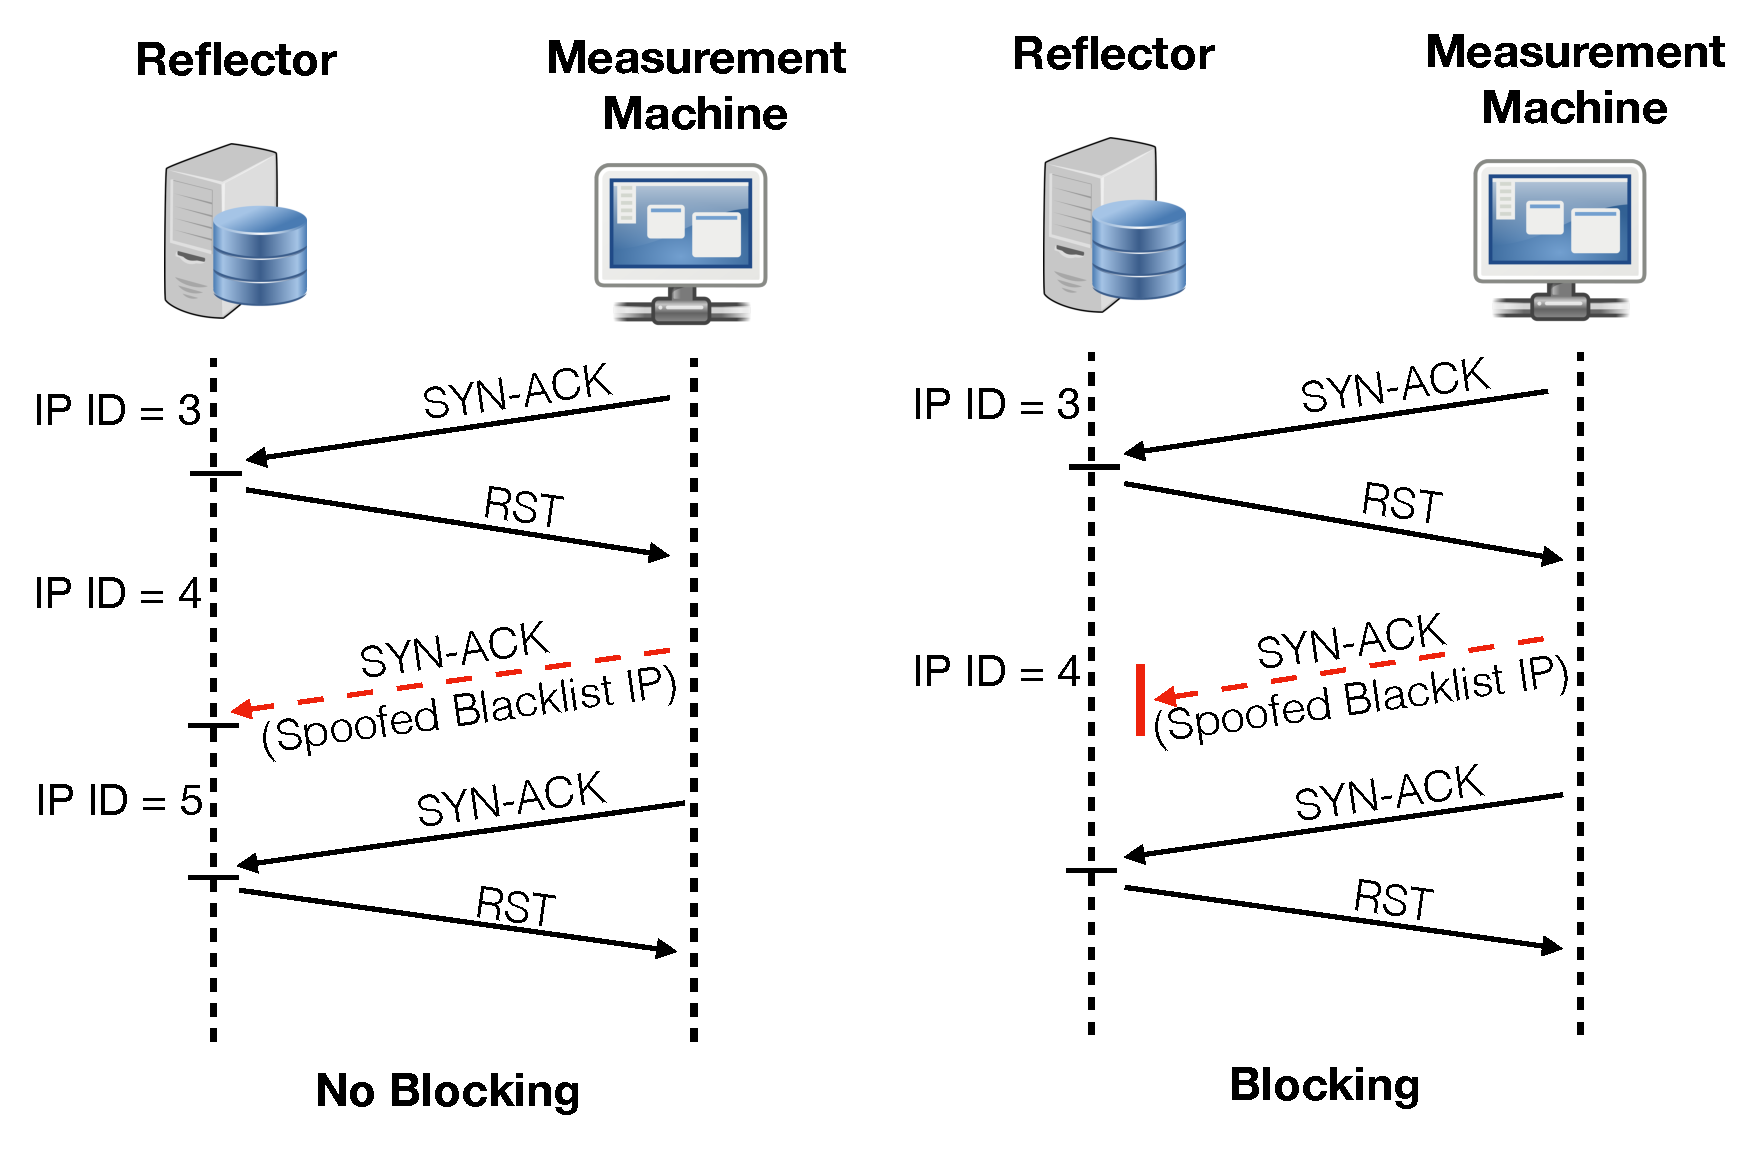
\includegraphics[width=0.98\columnwidth]{data_usage/images/cropped_method_protocol_v2.pdf}
    \caption{The basic method to detect network blocking using the IP ID side channel.}
    \label{fig:coreidea}
\end{figure}

In an ideal world, where there is no packet loss during transmission
and no extra traffic on the {\reflector}, one would see a clear difference
in the IP IDs from the responses between the two different scenarios.
In particular, I expect the {\reflector} to send a RST response for
each SYN-ACK packet I send, and I will receive the responses for
the SYN-ACK with the measurement machine's source address. The IP IDs of 
these received RST packets will reflect the number of packets sent by the
reflector. If the reflector did not receive the SYN-ACK packets with the
blacklist IP as source addresses(because they were blocked by a
firewall), the IP ID sequence in the RST responses will be an
increasing sequence without gaps (the ``Blocking'' case in Figure~\ref{fig:coreidea}).
On the other hand, if the reflector did
receive the SYN-ACK packets with the blacklist IP, it would have sent
a RST packet in response to each such packet, incrementing the IP ID counter
each time. While I will not see the RST packets sent to the blacklist
IP, I \emph{will} observe the increments in the IP ID sequence.
More specifically, one would see a gap in the IP ID sequence of packets
received by the measurement machine (the ``No Blocking'' case in
Figure~\ref{fig:coreidea}).
These two cases, illustrated in Figure~\ref{fig:coreidea}, allow us to
determine whether a particular blacklist IP is blocked by some network
device, such as a firewall, somewhere between the measurement host and
the reflector. When there is no blocking in place (left), the measurement
machine will see an IP ID gap in two RST responses: the second IP ID will
increase by two. Whereas if there is network blocking (right), then the
two IP IDs will not have a gap: the second IP ID will only increase by
one.
%and this gap should equal the number of RST
%packets sent to the blacklisted addresses, which, in turn, should equal the
%number of SYN-ACK packets received by the reflected with the blacklisted
%address.

This measurement technique is inspired by the method proposed in previous
work~\cite{ensafi2014detecting, pearce2017augur}. However, to make it work 
for my objective I need to handle a few more important issues, as I will
see in the rest of this section.

\subsection{Compare with Previous Method}

At a high level, the objective of the measurement is to determine, from a third
point, if a {\reflector} blocks a blacklist IP. The blocking behavior that we
want to measure is \textit{inbound blocking} -- that is the incoming traffic
is blocked and as a result traffic does not reach the intended host. A
typical example is a network firewall, where it can stop certain network
packets from reaching hosts behind the firewall. Here we abstract the
{\reflector} as $Host_A$, blacklist IP as $Host_B$, and the problem is to
detect the connectivity between two hosts on the Internet.

%Another type of blocking is %\textit{outbound blocking}, where the outgoing
%traffic to a ``blocked host'' from a host within the network is blocked. %A
%typical example is network censorship. Our measurement in this paper only
%focuses on inbound blocking, %and we will explain more about this in the
%following sections.

\begin{figure}[t]
\centering
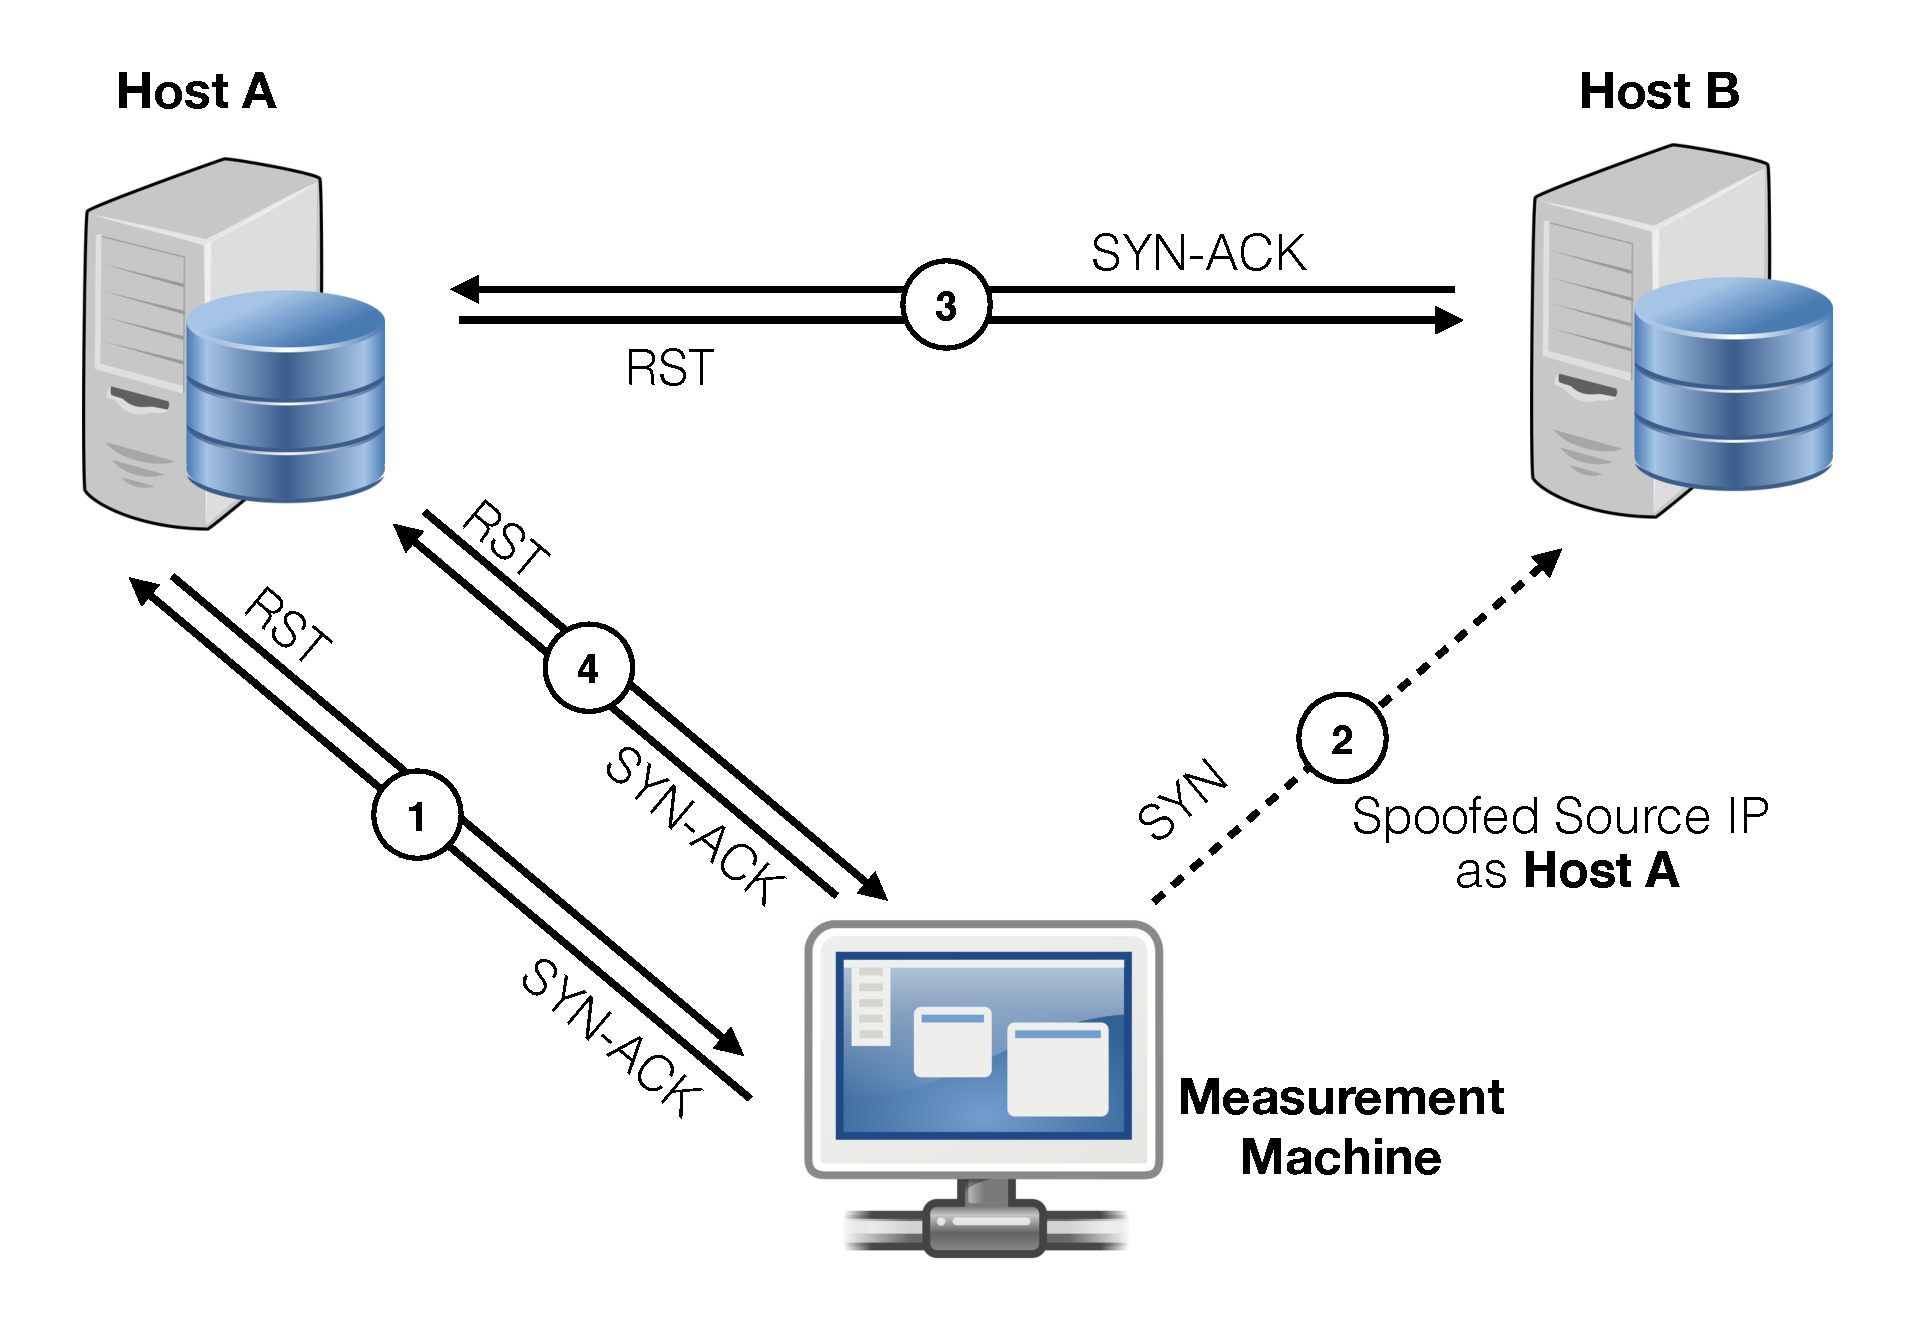
\includegraphics[width=0.8\columnwidth]{data_usage/images/croped_method_old.pdf}
\caption{Measurement method used in previous work.}
\label{fig:old_method}
\end{figure}

In previous works~\cite{pearce2017augur, ensafi2014detecting}, to measure
the connectivity between two hosts from a third party, they send spoofed packets
to impersonate one of the hosts. This methodology -- one we refer
to as the \textit{triangle measurement} takes advantage of the TCP 3-way
handshake protocol, as shown in Figure~\ref{fig:old_method}.

The measurement machine first sends a probe to the $Host_A$, in this case a TCP
SYN-ACK packet. $Host_A$ responds with a RST packet since it received a SYN-ACK
without the preceding SYN packet. Thus, the measurement machine gets the
first IP ID $IP\mhyphen ID_1$ from the RST packet (corresponds to Step 1 in
the figure). Next, the measurement machine sends a spoofed TCP SYN packet to
$Host_B$, with source IP address set to the IP address of $Host_A$ (Step 2).
$Host_B$ then sends a responding SYN-ACK packet to $Host_A$, which causes $Host_A$
to respond with a RST packet (Step 3), and increment its IP ID counter by 1.
Finally, the measurement machine probe $Host_A$ again and get the second IP ID
$IP\mhyphen ID_2$ (Step 4).

Now we can infer whether $Host_A$ is inbound blocking traffic from $Host_B$ by
observing the difference between $IP\mhyphen ID_1$ and $IP\mhyphen ID_2$.
Assuming there is no packet loss, and that $Host_A$ does not have any extra
traffic besides our measurement traffic, then
$IP\mhyphen ID_2 = IP\mhyphen ID_1 + 2$ implies there is no inbound blocking,
since it indicates that $Host_A$ received both packets in step 3 and step 4,
while $IP\mhyphen ID_2 = IP\mhyphen ID_1 + 1$ means there is blocking.

Previous work chose this ``triangle measurement'' because it ensures that in
step 3, the packets from $Host_B$ will go through the same routes as the
traffic originated from $Host_B$. So from $Host_A$'s perspective, it can not
identify that the traffic from $Host_B$ are spoofed. However, in this schema,
one hard requirement is that $Host_B$ needs to be active and responding to TCP
SYN probe. This is not an issue for censorship measurement, as $Host_B$ in this
case are popular sites (Google, Facebook, Twitter etc.) that guaranteed will
respond to SYN probe.

However, in our case, we need to measure whether $Host_A$ is blocking traffic
from a blacklist IP($Host_B$). But there is no guarantee that these IP
addresses are active and thus may not respond to our SYN probe. In fact, we
found that the percentage of responding IPs in a blacklist can be as low as less
than 20\%. This dramatically reduces the candidate IPs we can sample from a
blacklist to test, especially for small blacklists that only have a few hundred
IPs. Furthermore, there are many other additional constraints when shortlisting
IPs for measurement from a blacklist.
The requirement that blacklist IPs respond to SYN probe does not work for our
use case. 
%\textcolor{red}{Explain the choice for only inbound blocking}

In order to get around this limitation we adjust the measurement methodology.
In this new methodology, the measurement machine directly sends spoofed
packets to the target host, as shown in Figure~\ref{fig:new_method}. In
this case, the measurement machine first probes $Host_A$ to get the first IP ID
$IP\mhyphen ID_1$, then it sends a spoofed packet, with source IP set to
$Host_B$(Blacklist IP), directly to $Host_A$. Finally, it sends a second probe
to $Host_A$ and get the second IP ID $IP\mhyphen ID_2$. Now we can use the same
logic as before to infer whether $Host_A$ is inbound blocking $Host_B$. In this
approach, we do not require $Host_B$ to be actively responding SYN packets, any
IP address can be used here to conduct the test. The drawback is that the
spoofed packets now at times go through a different route versus the packets
originated from $Host_B$. Some network that implement spoofed packet
detection~\cite{ferguson2000rfc2827} could drop our spoofed packets, giving us
a false signal of inbound blocking. Therefore, when selecting hosts we conduct
extensive tests to weed out hosts that have such detection logic in place. We
find that not a lot of target hosts have such detection logic. We will talk in
detail about host selection in the follow sections.

%Therefore, we modified the measurement so that the measurement machine  directly
%send spoofed packets to host A, as shown in Figure~\ref{fig:new_method}. In
%this case, the measurement machine first probes host A to get the first IP ID
%\texttt{IP\_ID\_1}, then it sends a spoofed packet, with source IP as host B,
%directly to A. Finally, it sends a second probe to host A and get the second
%IP ID \texttt{IP\_ID\_2}. Now we can use the same logic as before to infer
%whether host A is inbound blocking host B. In this approach, we do not
%require host B to be actively responding SYN packets, any IP address can be
%used here to conduct the test. The drawback now is that the spoofed packets
%will likely go through a different route versus the packets originated from
%host B. Some network that implemented spoofed packet detection~\cite{ferguson2000rfc2827}
%could drop our spoofed packets, giving us a false
%signal of inbound blocking. Therefore, when selecting hosts for the
%measurement, we conduct extensive tests to make sure the hosts do not have
%such detection logic in place. Our experiment also shows that not a lot of
%hosts have such detection logic. We will talk in detail about host selection
%in Section~\ref{sec:requirement_host}.

\begin{figure}[t]
\centering
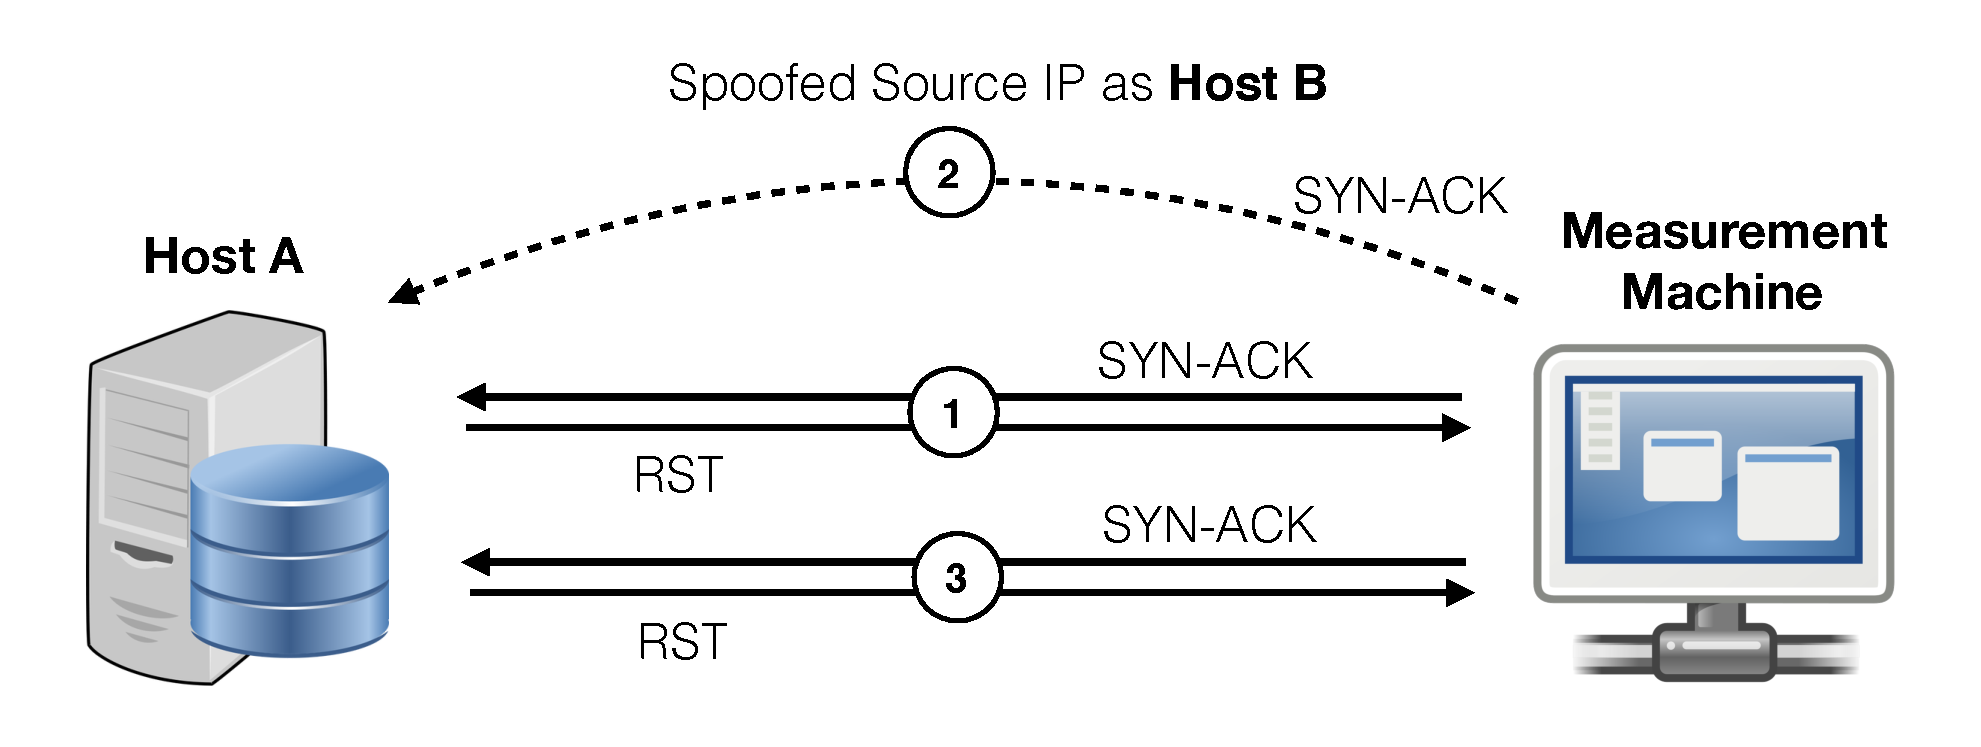
\includegraphics[width=0.8\columnwidth]{data_usage/images/croped_method_new.pdf}
\caption{Measurement method used in this work.}
\label{fig:new_method}
\end{figure}

\subsection{Finding Suitable Reflectors}
\label{sec:methrefl}

At a high level, my methodology relies on being able to infer blocking
using the IP ID side channel. Keeping that in mind, listed below is the
criteria I look for when scanning the Internet to search for suitable
reflectors.

\begin{itemize}
    \item \textbf{RST packet generation:}
    The {\reflectors} must reply with a RST packet to a TCP SYN-ACK packet 
    without an established connection. Some hosts drop incoming SYN-ACK 
    packets if there is no corresponding SYN packet. These hosts are not
    suitable for my measurement methodology. I choose SYN-ACK packets 
    instead of SYN because it does not create an intermediate state on the
    {\reflectors} and connection is terminated in one go.

    \item \textbf{Shared monotonic increasing IP ID counter:}
    The IP ID counter in the {\reflector} needs to be globally shared, so all
    network traffic generated from the host will use the same counter for IP
    ID assigning. It also needs to be monotonically increasing, so I can
    observe the number of packets generated by the host between two
    measurements using the difference of IP IDs.
    
    \item \textbf{Low traffic:}
    The technique requires the host to have low traffic volumes
    in general, since the technique depends on the fact
    that I can observe a clear difference in IP ID increases when sending
    spoofed packets. If there are always many other
    packets coming to the host, it would be infeasible to observe the IP ID
    changes triggered by the measurement packets.

    \item \textbf{No ingress filtering:}
    I send spoofed packets to {\reflectors} to infer traffic blocking.
    However, some network providers utilize ingress filtering techniques and
    drop packets once they detect the packets are not from the networks they
    claimed to originate. This would cause the spoofed packets being dropped
    and give us a false signal of traffic blocking.

    \item \textbf{No stateful firewall blocking:}
    Some networks deploy a stateful firewall that blocks access from a source
    IP after receiving too many repetitive packets. One example is to defend
    against SYN floods~\cite{lemon2002resisting}. While I try to keep the
    number of the measurement packets as low as possible, if the spoofed
    packets trigger such firewall rules and then I are blocked by the 
    firewall, I will incorrectly conclude that the {\reflector} uses a
    blacklist to block that IP.
\end{itemize}

I try to uncover how online hosts are using IP blacklists to
block traffic. But when looking at the problem on a global scale, there are
many policy related reasons why a host blocks network traffic,
such as censorship. These alternate sources of blocking could disrupt the
measurement, making it hard to distinguish the type of security-related 
blocking I target. To simplify the problem, in this chapter I focus on 
the hosts in United States.

I find {\reflectors} in the United States with open ports using a snapshot
of Censys~\cite{censys} scanning data from November 8, 2019. Then I scan 
these 40 million hosts to identify the ones with the IP ID side channel. 
I send multiple probes to each host targeting an open port from different
source addresses, and then check IP IDs in the responses. In the case where 
hosts have multiple open ports, I randomly select a port to send the probe.

To identify stateful firewalls, I send SYN-ACK packets to each {\reflector}
in two different patterns: 1 second per packet with 24 packets, and 5 packets
per second with 60 packets, which corresponds to the speed I probe
{\reflectors} during actually experiments (see the following section). I
repeat each experiment 6 times and discard the hosts that block us after the
experiment. To find the hosts with low extra traffic, I send 24 probes
to each host, 1 per second, and repeat the experiment 5 times at different
times of the day. I then collect the result and only select the hosts where
more than 30\% of their IP ID increases are equal to 1 per second --- that is,
the host did not receive any extra traffic besides my probes,
and all of the increases were smaller than 10 within a second.

Finally, I try to identify hosts experiencing ingress filtering. To
account for differences in ingress filtering that may possibly occur on
different network paths to the {\reflectors}, I acquired 7 vantage points 
around the world to exercise different paths. These vantage points are
from the US west coast, east coast and midwest, and places in Asia, Europe,
Australia and South America.

I then send spoofed packets from my measurement
machine to the {\reflectors} with spoofed source addresses corresponding to
the 7 vantage points, and later collect responses at each vantage point.
I only select the {\reflectors} that send responses to all 7
vantage points, meaning they did not drop spoofed packets on these network paths.

Eventually, I identified {\reflcount} IP addresses in US that meet the
requirements.\footnote{I initially discovered more than 300K {\reflectors}, 
but during my experiments some hosts became inactive. The number reported 
here is the final number after I finished all the experiments.} For the 
purpose of this chapter, here I treat each individual IP address as a 
distinct {\reflector}. Detailed numbers are presented in
Table~\ref{tab:target-hosts}.

\begin{table}[t]
\centering
\caption{The number of {\reflectors} (IP addresses) identified in the United States, and the
corresponding count of /24 prefixes and Autonomous Systems.}
\begin{tabular}{l >{\hfill}p{4.5cm}}
 \toprule
 Category                    &  Count    \\
 \midrule
 \textbf{IP Addresses}       &  \reflcount  \\
 \textbf{/24 Count}          &  128,712  \\
 \textbf{Autonomous Systems} &  3,371    \\
%% \textbf{Organizations}      &  3,321    \\
 \bottomrule
\end{tabular}
%% and organizations (One organization can have multiple ASes)}
\label{tab:target-hosts}
\end{table}

\subsection{Choosing the Blacklists}
\label{sec:methblkl}
%By far I have demonstrated the methodology and the requirements for selecting
%measurement candidates. One question I have not addressed is what IP blacklists
%I choose to test against. Section~\ref{sec:methodology} described the criteria
%for sampling blacklist IPs from a given blacklist, but I still need to pick
%the blacklist in the first place.

\begin{table}[t]
\centering
\caption{Top {\blacklistnum} popular public IP blacklists.}
\begin{tabular}{l r}
 \toprule
\textbf{Blacklist}   & \quad\quad \textbf{Average Number of IPs} \\
 \midrule
 \textbf{\spamhausdrop}                 & $\sim$ 20,000,000       \\
    \multicolumn{2}{l}{    Spamhaus Don't Route Or Peer Lists}  \\
    %\hspace{0.2cm}    https://www.spamhaus.org/drop/drop.txt \\

 \textbf{\spamhausedrop}                &  $\sim$ 900,000          \\
    \multicolumn{2}{l}{    An extension of the Spamhaus DROP list} \\
    %\hspace{0.2cm}    https://www.spamhaus.org/drop/edrop.txt \\

 \textbf{\dshieldtop}                   &  5,120            \\
    \multicolumn{2}{l}{    DShield.org recommended top 20 /24s to block} \\
    %\hspace{0.2cm}    https://www.dshield.org/block.txt \\

%\textbf{\ciarmy}                       & 15,000            \\
    %\multicolumn{2}{l}{    Collective Intelligence Network Security(CINS) blacklist} \\
    %\hspace{0.2cm}    http://www.ciarmy.com/list/ci-badguys.txt \\

 \textbf{\etcompromised}                & $\sim$ 400               \\
    \multicolumn{2}{l}{    EmergingThreats.net recorded compromised hosts} \\
    %\multicolumn{2}{l}{\hspace{0.2cm} https://rules.emergingthreats.net/blockrules/compromised-ips.txt} \\

 \textbf{\snortfilter}                  & $\sim$ 1,500             \\
    \multicolumn{2}{l}{    labs.snort.org supplied IP blacklist}  \\
    %\hspace{0.2cm}    http://labs.snort.org/feeds/ip-filter.blf \\

 \textbf{\bdsatif}                      & $\sim$ 6,000             \\
    \multicolumn{2}{l}{    Binary Defense System ban list} \\
    %\hspace{0.2cm}    https://www.binarydefense.com/banlist.txt \\

 \textbf{\feodo}                        & $\sim$ 700              \\
    \multicolumn{2}{l}{    Abuse.ch Feodo tracking list}  \\
    %\hspace{0.2cm}    https://feodotracker.abuse.ch/downloads/ipblocklist.txt \\

 \textbf{\blocklistde}                  & $\sim$ 30,000           \\
    \multicolumn{2}{l}{    Blocklist.de blacklist IPs} \\
    %\hspace{0.2cm}    http://lists.blocklist.de/lists/all.txt\\

 \textbf{\ettor}                        & $\sim$ 6,000             \\
       \multicolumn{2}{l}{ IPs that belong to Tor network (not just exits node)}  \\
       %\multicolumn{2}{l}{\hspace{0.2cm}    https://rules.emergingthreats.net/blockrules/emerging-tor.rules} \\
 \bottomrule
\end{tabular}
\label{tab:target-blacklists}
\end{table}

I choose candidate blacklists from public IP blacklists since I
do not have access to commercial blacklists. In this work, I use the
FireHOL IP blacklist collection~\cite{firehol} which aggregates over 
100 public IP blacklists. However, I cannot reasonably test against 
all the blacklists and so, for the purposes of this chapter, I would 
like to select the most popular public IP blacklists and then do a 
more detailed measurement of them.

For each of the public IP blacklists, I sample five IPs (using the criteria
in Section~\ref{sec:methtarg}) from each list and test how many {\reflectors}
block all sampled blacklist IPs in each blacklist (using the method in
Section~\ref{sec:methtrain}). With this experiment, I
generate a list of the most popular blacklists. Of course, five sample points
from one list is not a strong enough indicator to conclude whether a host is
using that blacklist or not. That said, the goal of this measurement is not to
identify the exact hosts that use each blacklist. Rather, it is
estimate how widely used these blacklists might be so that I can use them for more detailed measurements. I
repeat the measurement twice and select the top {\blacklistnum} popular
blacklists,\footnote{I initially selected 10 blacklists. However, one blacklist,
abuse.ch Ransomware List, was discontinued by the provider during my
experiments, and so I removed that blacklist from consideration.} as listed in
Table~\ref{tab:target-blacklists}.

Note, the {\ettor} is the combination of three Tor blacklists, as they mostly
have the same content. This is primarily done since the huge overlap between
the three lists means that I have very few blacklist IPs that meet my
exclusive criteria (see Section~\ref{sec:methtarg}). The {\ettor} essentially
includes IPs for all nodes in the Tor network, including entry nodes, so the
{\reflectors} who block IPs on this list can neither be accessed from Tor nor
use Tor services themselves.

\subsection{Sampling Blacklist IPs}
\label{sec:methtarg}

For determining if a {\reflector} uses a particular IP blacklist, I use a
sample of IPs from the blacklist to test since it is infeasible for us to
test all blacklist IPs. Further, to obtain a definitive signal from my
measurement, I adhere to the following constraints when sampling blacklist
IPs:

\begin{itemize}
    \item \textbf{Exclusive:}
    A blacklist can share part of its contents with other blacklists. To
    reasonably infer whether a {\reflector} is using a specific blacklist, I
    need to test with the IPs that are unique to that blacklist --- IPs that are
    only in this blacklist, but no others.

    \item \textbf{Stable:}
    The IPs on a blacklist change over time. To reliably measure if a
    {\reflector} blocks IPs from a certain blacklist, I need the
    sampled IPs to stay in the blacklist throughout the measurement. I discard
    any measurements where the blacklist IP does not remain on the blacklist for
    the duration of the measurement.

    \item \textbf{Routable:}
    IP blacklists can contain unroutable IPs~\cite{li2019reading}. Sending
    packets with an unroutable source address results in a large portion of
    packets being dropped (which could potentially happen at the end ISP or 
    the transient link). Packet drops due to unroutable IPs would create 
    noise in the measurement. Therefore, when sampling IPs from blacklists I
    ensure that the IPs are routable.

    \item \textbf{Geo-location diversified:}
    Besides blacklisting, another common reason for a host to block certain
    traffic is geo-blocking, where a host blocks all traffic coming from a 
    certain country or a certain region. To minimize the effect of 
    geo-blocking, I prioritize IPs that are from the United States when 
    sampling IPs. The assumption is that a host in the US will not block 
    traffic from its own country. For IPs from other countries, I try to 
    increase the diversity of IP locations, making sure these IP are not 
    concentrated in a few countries when possible.

    \item \textbf{Not from the hosts' network (AS disjoint):}
    I observed many networks drop spoofed packets when the spoofed source 
    addresses are within their own network. So when selecting IPs, I make 
    sure that these IPs are not from the same ASes as one of the {\reflectors}.

\end{itemize}

To obtain ``exclusive'' IPs from a blacklist, I would potentially need an
``oracle'' that includes all IP blacklists, which is impractical. In this work,
I use the public IP blacklists collected by FireHOL, as mentioned earlier, to calculate the
exclusive part of each target blacklist. For ``stable'' IPs, I
collect all the target blacklists hourly, and ensure the sampled IPs are in
the blacklist through the duration of the experiment. To satisfy the
``routable'' requirement, I use the daily RouteView data~\cite{Routeview}
to identify BGP routable IPs. As for geo-location diversity, I use
Netacuity~\cite{netacuity} to make sure for each experiment the sampled IPs
cover as many different countries as the data allows.


\subsection{Experiment Design}
\label{sec:methtrain}

Previously, I described the ideal model of the measurement method,
which explained the idea and workflow at a high-level. However, this model
does not take into consideration packet loss or extra traffic at the
{\reflector}. As one would expect, these assumptions are unrealistic in a real
world scenario, as packet loss can happen at many stages along the path.
Furthermore, there is no guarantee that the host with an open port online
will not receive any other traffic. Thus, to perform the measurement in the real
world, I need to take all these factors into consideration and make sure
that the analysis model is robust to these real world uncertainties.

Moreover, the detection methodology also needs to be \textit{efficient},
\textit{accurate}, and have \textit{low overhead}. Since I need to
measure every pair of \texttt{({\reflector}, IP)}, which is a
very large number, and the blacklist content changes rapidly, the detection
method needs to be efficient so that I can finish the measurement in a
reasonable amount of time. The method should also have a low false positive
and false negative rate, so I can be confident about the result. Finally, it
should require as few packets as possible, both to meet network bandwidth
limitations on the measurement machine side and reduce impact on
{\reflectors}.

I define a \textit{trial} as a single measurement that tests if a
{\reflector} blocks a blacklist IP. Figure~\ref{fig:design_implementation}
shows the process of one trial in detail. 
The solid blue lines are the \textit{probe
packets}. Dashed red lines are the \textit{spoofed packets}. The spoofed
packets impersonating blacklist IPs trigger the increase of the
{\reflectors}' IP ID. The IP ID of responses to probe packets are used to
determine blocking behavior.
For each trial, the measurement
machine sends five consecutive \textit{probe packets} to the {\reflector},
with each packet being sent one second apart. In the experiment, the probe
packets are TCP SYN-ACK packets and I get IP IDs from response RST packets.
Between the third and fourth probe packets, the measurement machine sends
five \textit{spoofed packets}, also TCP SYN-ACK, with source IPs equal to the
blacklist IP. And between the fourth and the fifth probe packets, it sends
another five spoofed packets. Each time I send the five spoofed packets, I
send them 0.15 second apart consecutively, spreading them across the one-second
window between two IP ID probes.

\begin{figure}[t]
\centering
\includegraphics[width=0.85\columnwidth]{data_usage/images/croped_design_implementation.pdf}
\caption{Blocking detection methodology.}
\label{fig:design_implementation}
\end{figure}

Now, I inspect the increases between the IP IDs for the packets received by the
measurement machine. In an ideal world, when there is no other traffic
generated by the {\reflector}, and no packet loss during the measurement, one
should observe that the IP ID increases between consecutive probes by exactly
1, and for the last two deltas, since I send the spoofed packets in between
the probe packets, the final IP ID increases will be different based on the
host's blocking behavior.

If the {\reflector} does not block the blacklist IP, then
I will observe an IP ID increase sequence in the received RST responses as:
\[[\hspace{0.1cm} +1, +1, +6, +6 \hspace{0.1cm}]\]
Here the last two deltas are +6 since the {\reflector} does not block the
blacklist IP and thus responds to spoofed packets, causing IP ID to increase by
5, and the probe packet causes it to increase by another 1, which together make +6.

On the other hand, if the {\reflector} blocks the blacklist IP, then I will see an IP
ID increase sequence as:
\[ [\hspace{0.1cm} +1, +1, +1, +1 \hspace{0.1cm}] \]
Here the last two deltas are +1 since the {\reflector} blocks the blacklist IP,
leading to no extra change in IP ID.
%\textcolor{red}{maybe have an example of what happens when I do not see ideal conditions}

The first three probes --- corresponding to the first two IP ID deltas --- act as a
control. The last two ``probe and spoof'' patterns perform the actual measurement.
Seeing the initial two ``+1'' indicates this host is in a quiet period --- no
extra network traffic. Therefore, I can be more confident that the following
IP ID jump (``+6'' in this case) is because of the experiment. However,
while I present the choice of the numbers in the experiment as fait accompli,
there is a rationale behind the choice of numbers which I discuss in Section~\ref{subsec:fpfn_analysis}.

\subsubsection{Inference Criteria}
%\textbf{Inference Criteria: }
Now I discuss how to infer whether a {\reflector} is blocking a blacklist IP
in the real world. I have limited vantage points from the measurement machine, as
such, and my information is limited to the IP IDs I see from the {\reflector}.
Therefore, I would like to be very conservative when making a judgment. In this
measurement, my approach is to try the same trial, between a {\reflector} and a
blacklist IP, many times until I get a ``perfect signal'' --- a response
which matches all the criteria below:

\begin{enumerate}
    \item The measurement machine received exactly five RST responses from the {\reflector}.
    \item The five responses are received one second apart consecutively.
    \item The IP ID increase sequence in the five responses are either [+1, +1, +6, +6],
    which I will conclude as no blocking, or [+1, +1, +1, +1], which I will
    conclude as blocking.
    \item If any of the above three criteria are not met, I repeat the same experiment
    again. I repeat up to 15 times before giving up.
\end{enumerate}

Essentially, the first requirement ensures no packet loss. The second
requirement ensures responses I received reflect the real IP ID changes in
the {\reflector}. The Internet does not guarantee the order of packet arrival.
Although I send one probe packet per second, and send the spoofed
packets in between of the probe packets, these packets might not arrive at
the {\reflector} in the same order. There is a similar case for response packets.
Therefore, the IP ID sequence I get from the response packets
might not represent the real order of IP ID changes in the host. Requiring
that
the received response packets are also close to 1 second apart, I minimize
the probability of the reordered packets. In my experiment, I enforce that
the response packets can not be less than 0.85 or more than 1.15 seconds
apart.

The third requirement is the core of my inference logic. I want to be
conservative when concluding whether there is blocking or not, so I will
make the judgment only when I observe an IP ID increase sequence [+1, +1, +1,
+1] or [+1, +1, +6, +6], and ignore everything else. Then if I saw a
sequence of [+1, +1, +1, +1] but the host is not blocking the blacklist IP,
that would mean all the 10 spoofed packets were lost during the transmit. On
the other hand, if I see [+1, +1, +6, +6] and the host is actually blocking
the blacklist IP, then that would mean during the experiment, there are
exactly five extra packets generated by the host during each of the last two
windows. Both cases are very unlikely to happen, and I will show a concrete
analysis of false positives and false negatives in the remainder of this section.


\subsubsection{False Positive and False Negative Analysis}
\label{subsec:fpfn_analysis}
%\textbf{False Positive and False Negative Analysis: }
For the experiment, a ``false positive'' is when a host is not
blocking a blacklist IP, but I mistakenly conclude it is blocking. On the
other hand, a ``false negative'' is when a host is blocking a
blacklist IP, but I mistakenly conclude it is not blocking. With
{\reflectors} being collected, I can empirically evaluate the
probability of a false positive or a false negative precisely.

For false positive evaluation, I first acquire a list of IPs that are verifiably
not being blocked by {\reflectors}. Since I own these IPs, I can easily verify
that by directly probing {\reflectors} from these IPs. I acquired and tested
1,265 IPs from five different /24s. Then I probe {\reflectors} and send the
spoofed packets with source addresses set to these pre-selected IPs. Since I
know that these IPs are not blocked, if I observe an IP ID increase sequence of
[+1, +1, +1, +1], then I know it is a false positive.

For false negative, I run the experiment with only probe packets, and no
spoofed packets. This is equivalent to the scenario where the host blocks the
spoofed IP. Then if I observe an IP ID increase sequence of [+1, +1, +6,
+6], then I know it was due to the background traffic at the {\reflector}
and hence is a false negative.

Although I have presented the design where I spoof five packets
in each of the last two seconds, I also experimented with a range of
numbers and calculated their false positive and negative rates. I tested
with spoofed packets equal to 3, 4, 5, 6, 7 respectively. For each number,
I use 15 distinct IPs I own as the source addresses to spoof, and I
create another group with 15 place holder IPs where I do not send spoofed
packets during the experiment. I run each experiment twice, and the final
results are shown in Figure~\ref{fig:fp_fn_analysis}.

%Our goal is to minimize the false positives and false negatives while also keeping
%in mind the amount of traffic I generate. Additionally, I have a few dimensions
%of the experiment which I can adjust to reach this goal. Namely, the number of
%packets I spoof, and the number of times I spoof.
%To find these optimal numbers, I test with a range of numbers and calculate

\begin{figure}[t]
\centering
\includegraphics[width=0.85\columnwidth]{data_usage/images/false_positive_negative.pdf}
\caption{False positive rates and false negative rates of the technique when spoofing different amount of packets.}
\label{fig:fp_fn_analysis}
\end{figure}

A few things stand out. The false negative rate drops significantly when I
send 5 spoofed packets. Surprisingly, the false negative rate jumps up
slightly when I spoof 6 packets. On the other hand, the false positive rate
keeps marginally trending downwards as I increase the number of spoofed
packets. I try to make the trade-off between having low false positive and
negative rates, but at the same time generating as little traffic as possible.
I choose 5 spoofed packets as a balance. By sending 5 spoofed packets, I
get a false positive rate of 2.5e-5, and a false negative rate of 8.5e-5.

Furthermore, I also experimented with strategies where I send 4 probe packets, from which
I get 3 IP ID deltas, and sending 6 probe packets, from which I get 5 IP ID
deltas. With only 3 deltas I suffer a higher false negative rate, as it is
easier for the {\reflector} to show the same IP ID increase sequence with
extra traffic. With 6 probes, on the other hand, I prolong the experiment,
and more importantly, it is harder for us to get the ``perfect signal'' since
it is harder to capture a period with no other traffic when the time window
is longer. Thus, the choice of 5 probe packets with 5 spoofed packets in
between is a trade-off between multiple factors.

%I choose to send 5 probe packets because it is a balance between getting
%enough sample point of IP ID to see the changes, and not sending too many
%packets to the {\reflector} that might affect the host, as I need to repeat
%the experiment many times for many different blacklist IPs. The first three
%probes (where I get the first two IP ID delta) act as a control, and the
%last two probe and the spoof packets serve the actually experiment. The
%choice of 5 spoofed packets between each second is also the result of
%balance. If I send too little spoofed packets, then it is hard to argue
%whether the additional IP ID increments come from our spoofed packets or the
%hosts' own third-party traffic. If I send too many spoofed packets, it is
%hard to ensure they will arrive the host exactly between the probe packets,
%and also might trigger some stateful firewall logic, as I discussed in
%Section~\ref{sec:requirement}.

\subsection{Control Group}
\label{sec:methvalid}
%\noteby{KL}{Here we
%    should describe additional validation, such as testing whether popular sites
%    are being blocked, and any other validation steps, such as repeating the
%    measurement, that I do. The part where I confirm our findings by asking
%    universities about their blocking policy can remain in the analysis section.}
To further validate the measurements, every time I test a set of
blacklist IPs against each reflector, I also include a control group
of 20 randomly chosen IPs. These IPs are chosen from networks
geo-located in the United States. I further ensure they do not
appear on any of the blacklists, they are BGP routable, and they are
not from the same ASes as the {\reflectors}. The purpose of the
control group is to create a random set of IPs that are unlikely to be
blocked in bulk by a {\reflector}. I use US IPs to avoid the
potential problem of geo-blocking. If a {\reflector} does block a
significant fraction of control IPs, it is probably because the
{\reflector} is not suitable for this methodology (one reason can be
that the ingress-filtering step did not catch these IPs). I discover
91 reflectors that constantly show blocking behavior for all control
IPs, while the remaining reflectors never block more than 10 of the
control IPs. I conclude that these 91 reflectors are not useful for
measurement, and remove them from the total reflector set.

\subsection{Ethical Considerations}
\label{sec:ethics}

In general, I believe the measurement would not cause much harm, as I only 
send TCP SYN-ACK packets to these hosts, without any other communication. Since
the reflectors are all active hosts on the public Internet, I believe it is
unlikely that any dramatic action will be taken if they only received SYN-ACK
packets but no other communication from blacklist IPs. I limited my
measurement within the United States to further reduce the potential impact.
However, admittedly the experiment may trigger security alerts, causing 
network administrators to spend time looking into these unnecessary alerts.
But to be further cautious, I take effort to minimize the
measurement packets I send to each reflector, as described in
Section~\ref{sec:methtrain}. Moreover, I will not disclose the exact
identity of any reflector in this chapter, and only report aggregated
numbers.

%\subsection{Tor Blacklist Placeholder}
%Note that the {\ettor} includes IPs from all nodes involved in Tor
%networks, including entry nodes, so the {\reflectors} who block this
%list cannot use Tor services themselves.  As a result, this Tor list
%is more broad than Tor exit blocking, in which a host only blocks exit
%nodes so other hosts cannot access their service from Tor (but the
%blocking host can still access the Tor network itself).
%\noteby{GV}{Why define the Tor blacklist here?  Perhaps move to
%  blacklist selection or validation?}

%\input{content/requirements.tex}
%\section{Experiment Implementation}
\label{sec:implementation}
\noteby{KL}{This section will be deleted. Leaving it in for now so Vector can cut and paste from it.}

Section~\ref{sec:methodology} introduced the methodology at a conceptual level.
However, as with any real world measurement, we need to account for different
possible scenarios, and also take into consideration what works best with the
{\reflectors}. In this section, we first explain the implementation detail of
our {\reflector} selection, then we discuss the design of the blocking detection
experiment and false positive and false negative evaluation. Finally, we look
at how to exactly sample IPs from blacklists.

%\subsection{Measurement Infrastructure}
%Even at the conceptual level, it is evident that the measurement hinges
%on our ability to do two things. One, spoof IP addresses. Second, the
%ability to send many ``probe'' packets to hosts without getting blocked.
%For the first we got two machines that allowed us to spoof IPs outside
%our organization's source address validation zone. For the second part,
%we leveraged unused address space in the address space controlled by our
%organization. We configured multiple /24s to effectively point to a single
%machine so that we could cycle through many IPs from different /24s so that
%we do not burn our IPs.
%\textcolor{red}{maybe change organization to university?}
%\textcolor{red}{maybe have a small figure?}

\subsection{{\reflectorcap} Selection}

We use the daily scanning data from Censys~\cite{censys} as the starting point.
Censys scans the Internet daily and maintains a list of the daily active hosts
and their open ports. We took a snapshot of the Censys data on
\textbf{November 8th 2019} and then filtered them so that we are only left
with US hosts, which leads to about 40 Million hosts. We then scan these hosts
and identify suitable candidates -- hosts which have a shared global
monotonically increasing IP ID counter. We achieve this by sending multiple
probes to each host targeting an open port from different source addresses
and observing the responses. In the case where hosts have multiple open
ports, we randomly select a port to send the probe.

To identify stateful firewall, we send SYN-ACK packets to each host in two
different pattern: 1 second per packet with 24 packets, and 5 packets per second
with 60 packets, which correspond to the speed we probe {\reflectors} during
actually experiments(see the following section). We repeat each experiment 6
times and discard the hosts that blocked us after the experiment. To filter out
the hosts with low extra traffic, we send 24 probe to each host, 1 per second,
and repeat the experiment 5 times(in different time of the day). We then
collect the result and only select the hosts where more than 30\% of their IP
ID increases are equal to 1 per second (meaning in that second, the host did not
receive any extra traffic besides our probes), and all of these changes are
smaller than 10 within each second.

Finally, we try to identify the hosts with ingress filtering. In order to account
for differences in ingress filtering that may possibly occur on different path
to the {\reflectors} we acquired 7 vantage points in order to exercise
different paths. We then send spoofed packets from our measurement
machine to the {\reflectors} with spoofed source IP address corresponding to
the 7 vantage points, and we finally collect responses at each of the 7
vantage points. We only select the {\reflectors} that send responses to all 7
vantage points, meaning they did not drop any of our spoofed packets.

Eventually, we identified {\reflcount} IP addresses in US \footnote{We initially
discovered more than 300K {\reflectors}, but during our experiments, some hosts
became inactive. The number reported here are the final number after we finished
all our experiments.} that meet our requirements.
For the purpose of this paper, here we treat each individual IP
address as a distinct {\reflector}. Detail numbers are presented in
Table~\ref{tab:target-hosts}.

\begin{table}
\centering
\caption{The number of {\reflectors}(IP addresses) identified in United States, and the
corresponding count of /24, Autonomous systems and organizations (One
organization can have multiple ASes)}
\label{tab:target-hosts}
\footnotesize
\begin{tabular}{l >{\hfill}p{4.5cm}}
 \toprule
 Category                    &  Count    \\
 \midrule
 \textbf{IP Addresses}       &  \reflcount  \\
 \textbf{/24 Count}          &  128,712  \\
 \textbf{Autonomous Systems} &  3,371    \\
 \textbf{Organizations}      &  3,321    \\
 \bottomrule
\end{tabular}
\end{table}



\subsection{Experiment Design}

Previously, we described the theoretical model of our measurement method,
which explained the idea and workflow at a high-level. However, this model
does not take into consideration packet loss and extra traffic at
$Host_A$. As one would expect this is an unrealistic assumption in a real
world scenario, as packet loss can happen at many stages during the transit.
Furthermore, there is no guarantee that the host with an open port online
will not get any other traffic. Thus, to perform the measurement in real
world, we need to take all these factors into consideration and make sure
that our analysis model is robust to these real world uncertainties.

Besides that, our detection methodology also needs to be \textit{efficient},
\textit{accurate}, and have a \textit{low overhead}. Since we need to
measurement every pair of \texttt{<{\reflector}, blacklist IP>}, which is a
massive number, and also blacklist content is changing rapidly,
the detection method needs to be efficient so that we can finish the
measurement in a reasonable amount of time. The method should also have a low
false positive and false negative rate, so we can be confident about the result.
Finally, it should requires as less packets being sent as possible, both to
meet network bandwidth limitation on our measurement machine side, and to
generate less noise to the {\reflectors}.

We define a \textit{trial} as a single
measurement that tests if a {\reflector} blocks a blacklist IP.
Figure~\ref{fig:design_implementation} shows the process of one trial in
detail. For each trial, the measurement machine sends 5 consecutive
\textit{probe packets} to the {\reflector}, with each packet being sent 1
second apart. In our experiment, the probe packets are TCP SYN-ACK packets
and we get IP IDs from responded RST packets. Between the 3rd and 4th probe
packets, the measurement machine sends 5 \textit{spoofed packets}, also TCP
SYN-ACK, with source IPs equal to the blacklist IP. And between the 4th and
the 5th probe packets, it sends another 5 spoofed packets. Each time we send
the 5 spoofed packets, we send them 0.15 second apart consecutively, making
them spread across the 1 second window between two IP ID probes.

\begin{figure}[t]
\centering
\includegraphics[width=0.85\columnwidth]{images/croped_design_implementation.pdf}
\caption{Blocking detection method used in this paper. The solid blue line present
the \textit{probe packets}, where we get the IP ID from the response, and dashed red line
present \textit{spoofed packets}, where we spoof packets impersonate IP from
blacklists, and trigger the extra changes of the {\reflectors}' IP ID.}
\label{fig:design_implementation}
\end{figure}

Now, we look at the deltas between the IP IDs for the packets received by the
measurement machine. In an ideal world, when there is no other traffic
generated by the {\reflector}, and no packet loss during our measurement, we
should observe that the IP ID increase between consecutive probes by exactly
1, and for the last two delta, since we send the spoofed packets in between
our probe packets, the final IP ID increases will be different based on the
host's blocking behavior.

If the host does not block the blacklist IP, then
we will observe an IP ID increase sequence in our received RST responses as:
\[[\hspace{0.1cm} +1, +1, +6, +6 \hspace{0.1cm}]\]
Here the last two deltas are +6 since the {\reflector} does not block the
blacklist IP and thus responds to spoofed packets, causing IP ID to increase by
5, and our probe packet causes it to increase by another 1, which gets us to +6.

On the other hand, if the host blocks the blacklist IP, then we will see an IP
ID increase sequence as:
\[ [\hspace{0.1cm} +1, +1, +1, +1 \hspace{0.1cm}] \]
Here the last two deltas are +1 since the {\reflector} blocks the blacklist IP,
leading to no extra change in IP ID.
%\textcolor{red}{maybe have an example of what happens when we do not see ideal conditions}

The first three probes -- corresponding to the first two IP ID deltas -- act as a
control. The last two ``probe and spoof'' patterns serve the actual measurement.
Seeing the initial two ``+1'' indicates this host is in a quiet period --- no
extra network traffic. Therefore, we can be more confident that the following
IP ID accelerate(``+6'' in our case) is because of our experiment. However,
while we present the choice of the numbers in the experiment as fait accompli,
there is a rationale behind the choice of numbers which we discuss later in
this section.

\textbf{Inference Criteria: }
Now we discuss how to infer whether a {\reflector} is blocking a blacklist IP
in real world. We have limited vantage point from the measurement machine, as
such, we have no knowledge of what happened on the {\reflector}, and our
information is limited to the IP IDs we see from the {\reflector}. Therefore,
we would like to be very conservative when making a judgment. In this
measurement, our approach is to try the same trial, between a {\reflector} and a
blacklist IP, many times until we get a ``perfect signal'' --- a response
which matches all the criteria below:

\begin{enumerate}
    \item The measurement machine received exact 5 RST responses from the {\reflector}.
    \item The 5 responses are received 1 second apart consecutively.
    \item The IP ID delta sequence in the 5 responses are either [+1, +1, +6, +6],
    which we will conclude as no blocking, or [+1, +1, +1, +1], which we will
    conclude as blocking.
    \item If any of the above 3 criteria is not met, we repeat the same experiment again.
    We repeat up to 15 times before giving up.
\end{enumerate}

Essentially, the first requirement ensures no packet loss. The second
requirement ensures responses we received reflect the real IP ID changes in
the {\reflector}. Internet does not guarantee the order of packet arrival.
Although we send one probe packet per second, and then send the spoofed
packets in between of the probe packets, these packets might not arrive at
the {\reflector} in the same order. Similarly, the response packets might be
reordered. Therefore, the IP ID sequence we get from the responded packets
might not represent the real order of IP ID changes in the host. Enforcing
the received response packets are also close to 1 second apart, we minimize
the probability of the reordered packets. In our experiment, we enforce that
the response packets can not be less than 0.85 or more than 1.15 second
apart.

The third requirement is the core of our inference logic. We want to be
conservative when concluding whether there is blocking or not, so we will
make the judgment only when we observe an IP ID delta sequence [+1, +1, +1,
+1] or [+1, +1, +6, +6], and ignore everything else. Then if we saw a
sequence of [+1, +1, +1, +1] but the host is not blocking the blacklist IP,
that would mean all the 10 spoofed packets were lost during the transmit. On
the other hand, if we see [+1, +1, +6, +6] and the host is actually blocking
the blacklist IP, then that would mean during our experiment, there are
exactly 5 extra packets generated by the host during each of the last two
window. Both cases are very unlikely to happen, and we will show a concrete
analysis of false positives and false negatives in the remainder of this section.


\textbf{False Positive and False Negative Analysis: }
For our experiment, we define ``false positive'' to be when a host is not
blocking a blacklist IP, but we mistakenly conclude it is blocking. On the
other hand, we define ``false negative'' to be when a host is blocking a
blacklist IP, but we mistakenly conclude it is not blocking. With
{\reflectors} being collected, we can actually empirically evaluate the
probability of a false positive or a false negative.

For false positive evaluation, we first acquire a list of IPs that are verified
not being blocked by {\reflectors}. Since we own these IPs, we can easily verify
that by directly probing the hosts from these IPs. We have acquired and tested
1,265 IPs from 5 different /24s. Then we probe {\reflectors} and send the
spoofed packets with source addresses being these pre-selected IPs. Since we
know that these IPs are not blocked, if we observed an IP ID delta sequence
[+1, +1, +1, +1], then it is a false positive case. For false negative, we run
the experiment with only probe packets, and no spoofed packets. This is
equivalent to the scenario when the host blocked the spoofed packets. Then if
we observed a delta sequence [+1, +1, +6, +6], then we know it was due to the
background traffic at the {\reflector} and hence is a false negative.

So far we have not explained our experiment design choice of spoofing 5 packets
per second. In fact, we tested with a range of numbers and calculated
their false positive and negative rates. We tested with spoofed packets equal
to 3, 4, 5, 6, 7 respectively. For each number, we use 15 distinct IPs we own
as the source addresses to spoof, and there is another group where we do not
spoof any packets. We repeat each test 4 times and do the overall experiment
twice. The final results are shown in Figure~\ref{fig:fp_fn_analysis}.

%Our goal is to minimize the false positives and false negatives while also keeping
%in mind the amount of traffic we generate. Additionally, we have a few dimensions
%of the experiment which we can adjust to reach this goal. Namely, the number of
%packets we spoof, and the number of times we spoof.
%To find these optimal numbers, we test with a range of numbers and calculate

\begin{figure}[t]
\centering
\includegraphics[width=0.85\columnwidth]{images/false_positive_negative.pdf}
\caption{False positive rate and false negative rate of the technique when
spoofing different amount of packets}
\label{fig:fp_fn_analysis}
\end{figure}

A few things stand out. The false negative rate drops significantly when we
send 5 spoofed packets. Surprisingly, the false negative rate jumps up
slightly when we spoof 6 packets. On the other hand, the false positive rate
keeps marginally trending downwards as we increase the number of spoofed
packets. We try to make the trade-off between having low false positive and
negative rates, but at the same time generating as less traffic as possible.
We choose 5 spoofed packets as a balance. By sending 5 spoofed packets, we
get a false positive rate of 2.5e-5, and a false negative rate of 8.5e-5.

Furthermore, we also tested strategies where we send 4 probe packets, from which
we get 3 IP ID deltas, and send 6 probe packets, from which we get 5 IP ID
deltas. With only 3 deltas we suffer a higher false negative rate, as it is
easier for the {\reflector} to show the same IP ID increase sequence with
extra traffic. With 6 probes, on the other hand, we prolong the experiment,
and more importantly, it is harder for us to get the ``perfect signal'' since
it is harder to capture a period with no other traffic when the time window
is longer. Thus, our choice of 5 probe packets with 5 spoofed packets in
between is essentially a trade off.

%We choose to send 5 probe packets because it is a balance between getting
%enough sample point of IP ID to see the changes, and not sending too many
%packets to the {\reflector} that might affect the host, as we need to repeat
%the experiment many times for many different blacklist IPs. The first three
%probes (where we get the first two IP ID delta) act as a control, and the
%last two probe and the spoof packets serve the actually experiment. The
%choice of 5 spoofed packets between each second is also the result of
%balance. If we send too little spoofed packets, then it is hard to argue
%whether the additional IP ID increments come from our spoofed packets or the
%hosts' own third-party traffic. If we send too many spoofed packets, it is
%hard to ensure they will arrive the host exactly between the probe packets,
%and also might trigger some stateful firewall logic, as we discussed in
%Section~\ref{sec:requirement}.


\subsection{Blacklist IP Sampling}
%How we selected the target blacklists
Given a blacklist feed to test, we need to ensure the sampled IPs meet the
requirements stated in Section~\ref{sec:requirement_list}. In order to
satisfy those requirements we need to utilize external data.

The ``exclusive'' requirement indicates that the IPs we used should be unique
to that blacklist -- that is no other blacklist that we have access to should
have them. In this paper, we utilize the FireHOL IP blacklist
collection~\cite{firehol}, a public service that collect data from over 100
public popular IP blacklists everyday. We use the public IP blacklists
collected by FireHOL to calculate the exclusive part of each target blacklist.

For the ``stable'' requirement, we collect all the target blacklists hourly,
and ensure the sampled IPs are in the blacklist throughout the corresponding
experiments.

To meet the ``routable'' requirement, we use the daily RouteView
Project~\cite{Routeview} data to identify BGP routable IPs, and further check
their whois record to confirm. For geo-location information, we use
Netacuity~\cite{netacuity} to identify each IP's location, and make sure for
each experiment, the sampled IPs cover as many different countries as the
data allows.

%\subsection{Representative}

%\subsubsection{Are reflectors representative}
%One concern is that our reflector selection biases our measurement to only
%include hosts that are low traffic. A second concern is if the networks are
%themselves representative?

%we are conservative in our reflector selection. One can imagine we relax our
%constraints and use a statistical approach to classify reflectors (as seen in
%Augur paper).

%Stats on reflector distribution.
%\subsubsection{Are blacklists representative}

%\section{Target Blacklist Selection}

%A large scale breadth study to get a sense for which are the most popular
%free blacklists that are being used.
By far we have demonstrated the methodology and the requirements for selecting
measurement candidates. One question we have not addressed is what IP blacklists
we choose to test against. Section~\ref{sec:methodology} described the criteria
for sampling blacklist IPs from a given blacklist, but we still need to pick
the blacklist in the first place.

Since we do not have access to commercial IP blacklists, we choose our
candidates from public blacklists. The FireHOL IP blacklist collection, as we
mentioned earlier, aggregates a comprehensive list of public IP blacklists, so
we will conduct our measurement against these blacklists. However, it would be
too expensive for us to test against all these blacklists. Furthermore, some
blacklists might not be used by many hosts to block traffic, which then would
not give us much insight about blocking behavior on the Internet.

In this paper, we would like choose the most popular public IP blacklists,
and conduct our measurement and analysis in detail regarding these
blacklists. To choose the most popular blacklist, we conduct our measurement
over 61 public IP blacklists from the FireHOL collection, and for each
blacklist, we sample 5 IPs from that list using the criteria specified
before. Here we only test 61 blacklists since some lists are obsolete now,
and we only focus on the currently active blacklists. 5 sample points from
one list is not a strong enough indicator to conclude whether a host is using
that blacklist or not, but the goal of the experiment is not to identify the
exact hosts that use a blacklist. Rather, it is to get a close estimation so
we can figure out the most widely used blacklists for later measurements. We
repeat this experiment twice and select the top {\blacklistnum} blacklists
\footnote{We initially selected 10 blacklists, but one blacklist, abuse.ch
Ransomware List, was discontinued by the provider during our experiments, so
we discard that list.}, as listed in Table~\ref{tab:target-blacklists}.

\begin{table}
\centering
\caption{Selected {\blacklistnum} popular public IP blacklist. {\ettor} here is
the combination of three Tor blacklists, as they are having mostly the same
content.}
\label{tab:target-blacklists}
\footnotesize
\begin{tabular}{l r}
 \toprule
 Blacklist   & \quad\quad\quad\quad\quad Average Number of IPs \\
 \midrule
 \textbf{\spamhausdrop}                 & $\sim$ 20,000,000       \\
    \multicolumn{2}{l}{    Spamhaus Don't Route Or Peer Lists}  \\
    %\hspace{0.2cm}    https://www.spamhaus.org/drop/drop.txt \\

 \textbf{\spamhausedrop}                &  $\sim$ 900,000          \\
    \multicolumn{2}{l}{    An extension of the Spamhaus DROP list} \\
    %\hspace{0.2cm}    https://www.spamhaus.org/drop/edrop.txt \\

 \textbf{\dshieldtop}                   &  5,120            \\
    \multicolumn{2}{l}{    DShield.org recommended top 20 /24s to block} \\
    %\hspace{0.2cm}    https://www.dshield.org/block.txt \\

%\textbf{\ciarmy}                       & 15,000            \\
    %\multicolumn{2}{l}{    Collective Intelligence Network Security(CINS) blacklist} \\
    %\hspace{0.2cm}    http://www.ciarmy.com/list/ci-badguys.txt \\

 \textbf{\etcompromised}                & $\sim$ 400               \\
    \multicolumn{2}{l}{    EmergingThreats.net recorded compromised hosts} \\
    %\multicolumn{2}{l}{\hspace{0.2cm} https://rules.emergingthreats.net/blockrules/compromised-ips.txt} \\

 \textbf{\snortfilter}                  & $\sim$ 1,500             \\
    \multicolumn{2}{l}{    labs.snort.org supplied IP blacklist}  \\
    %\hspace{0.2cm}    http://labs.snort.org/feeds/ip-filter.blf \\

 \textbf{\bdsatif}                      & $\sim$ 6,000             \\
    \multicolumn{2}{l}{    Binary Defense System ban list} \\
    %\hspace{0.2cm}    https://www.binarydefense.com/banlist.txt \\

 \textbf{\feodo}                        & $\sim$ 700              \\
    \multicolumn{2}{l}{    Abuse.ch Feodo tracking list}  \\
    %\hspace{0.2cm}    https://feodotracker.abuse.ch/downloads/ipblocklist.txt \\

 \textbf{\blocklistde}                  & $\sim$ 30,000           \\
    \multicolumn{2}{l}{    Blocklist.de blacklist IPs} \\
    %\hspace{0.2cm}    http://lists.blocklist.de/lists/all.txt\\

 \textbf{\ettor}                        & $\sim$ 6,000             \\
       \multicolumn{2}{l}{ IPs that are belong to Tor network(not just exits node)}  \\
       %\multicolumn{2}{l}{\hspace{0.2cm}    https://rules.emergingthreats.net/blockrules/emerging-tor.rules} \\
 \bottomrule
\end{tabular}
\end{table}

\section{Overall Reflector Blocking}
\label{sec:perfect-blocking}

% Although rather extensive,
The methodology provides the basis for performing blacklist blocking
measurements at scale: a measurement technique to confidently
determine whether a reflector is blocking a particular IP address, a
viable set of reflectors that are compatible with the technique, and a
set of public security-related blacklists that provide a large set of
candidate IPs that hosts might block.  In this section, I describe my
large-scale experiment that uses this methodology for determining
which reflectors block IPs on the public blacklists, and which IPs
they block. I then present the overall results of the blocking
behavior of reflectors, and subsequent sections explore the different
behaviors in more detail.

\begin{figure}[t]
\centering
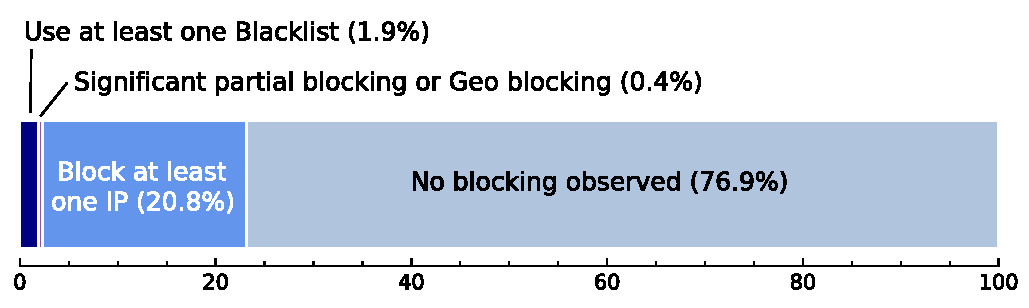
\includegraphics[width=0.95\columnwidth]{data_usage/images/reflector_breakdown_v2.pdf}
\caption{Breakdown of {\reflector} blocking based on three
  experimental runs.}
\label{fig:reflector-breakdown}
\end{figure}

For a particular experimental run, I randomly selected 25 IPs from
each blacklist that satisfies the requirements defined in
Section~\ref{sec:methodology}: exclusive, stable, routable,
geo-diversified, and AS disjoint. Then I evaluated the blocking
behavior for all {\reflroughnum} {\reflectors} against the 225
blacklist IPs sampled from all nine blacklists. To increase the chances
that these sampled IP will be stable, also to handle cases where reflectors
might update the blacklists slowly(a reflector might take a long time to
start blocking the newest IPs in a blacklist, although I discover
later that it is not the case, see Section~\ref{sec:latency-analysis}),
I ensure the sampled IPs have stayed in the blacklist for at least
2 weeks before the experiment. Since for each blacklist,
an experimental run can takes days to perform, as a post-processing step
I remove blacklist IPs from consideration that did not remain on the
blacklist for the duration of the experiment.

To increase the amount of evidence of blacklist blocking behavior, I
conducted three experimental runs, each time using a different set of 25
IPs from each blacklist. I then conclude that a {\reflector} is using a 
blacklist if only if all experiment runs show that it blocked all the 
sampled stable IPs from that blacklist.

I conducted the measurements from December 3--23rd, 2019.  During
this period, I tested 96,067,051 distinct \texttt{\small
  ({\reflector},IP)} pairs\footnote{The first two experiment I tested against
  all {\reflectors}, the last experiment I only tested against the ones that
  have shown blocking behavior in the first two tests}.
Based upon the criteria from
Section~\ref{sec:methodology}, I are able to conclusively determine
the blocking behavior (blocking or not blocking) of 98.3\% of the
tested pairs.  Among these pairs, 894,570 pairs display a
clear signal indicating ``blocking''.

Figure~\ref{fig:reflector-breakdown} presents the blocking behavior of
all 222,782 reflectors I tested partitioned into four categories:
those reflectors that I conclude use at least one of the public
blacklists (1.9\%), reflectors that block a large fraction of IPs on
at least one blacklist in every experiment(0.4\%, see more in
Section~\ref{sec:partial-blocking}), remaining reflectors that block at
least one blacklist IP (20.8\%), and reflectors that do not block any
blacklist IPs (76.9\%). (I identified 4,253 {\reflectors} that use at
  least one blacklist (Section~\ref{sec:blacklist-use}).  I also
  discovered reflectors that block a significant fraction of blacklist
  IPs, due in part to geo-blocking
  (Section~\ref{sec:partial-blocking}).  Finally, I identified a
  large number of reflectors blocking at least one IP, suggesting
  wider use of a much larger set of blacklists
  (Section~\ref{sec:large-scale}).) Note that given the requirements for hosts to
be reflectors, such as running old OS versions, it is not surprising a
large percentage shows no blocking of the blacklist IPs: they already
have attributes anti-correlated with high degrees of security hygiene.
Consequently, I want to emphasize that one should not conclude that
this percentage is representative of all hosts on the Internet.

These high-level results provide the foundation for additional
analyses and experiments, and going forward I further investigate
each of these categories of reflector blocking behavior in turn.
Section~\ref{sec:blacklist-use} explores blacklist use among the
{\reflectors}, Section~\ref{sec:partial-blocking} then examines
significant partial blocking behavior (including geo-blocking), and
Section~\ref{sec:large-scale} explores how reflectors that show any
blocking behavior can be used as evidence of much broader use of
blacklists.  As a final analysis, Section~\ref{sec:consistency}
studies the consistency of reflector blocking behavior at a coarser
granularity.

\begin{table}
\setlength{\tabcolsep}{4pt}
\centering
\caption{The number of {\reflectors} I conclude using each of the nine different
  blacklists, as well as the number of unique /24s and ASes those
  reflectors appear in.}
\begin{tabular}{l r r r}
 \toprule
 \textbf{Blacklist} (abbr.)   & \textbf{Reflectors}  & \textbf{/24s}   & \textbf{ASes}\\
 \midrule
 {\spamhausdrop} (DROP)                  & 4,142         & 1,782  & 50  \\
 {\spamhausedrop} (eDROP)                & 1,272         & 362    & 25  \\
 {\dshieldtop} (DTop)                    & 223           & 69     & 18  \\
 {\etcompromised} (ET)                   & 116           & 58     & 15  \\
 {\bdsatif} (BDS)                        & 85            & 41     & 3   \\
 {\feodo} (Feodo)                        & 64            & 26     & 16  \\
 %\textbf{\ciarmy}                              & 59            & 39 \\
 {\snortfilter} (Snort)                  & 52            & 20     & 11  \\
 {\blocklistde} (DE)                     & 36            & 18     & 8   \\
 {\ettor} (Tor)                          & 24            & 9      & 8   \\
 \midrule
 \textbf{Total Unique}                   & 4,253         & 1,827  & 77  \\
 \bottomrule
\end{tabular}

\label{tab:perfect-blocking-reflectors}
\end{table}

\section{Reflectors Using Blacklists}
\label{sec:blacklist-use}

In this section, I focus on the reflectors that use the blacklists I
study, including the relative popularity of the blacklists, patterns
in the use of multiple blacklists, and the rate at which reflectors
update.  I also use external sources of ground truth to validate my
findings.  Overall, I conclude from the results in this section that
my methodology is indeed effective at identifying blacklist use from
a remote third-party vantage point.

Recall that I use three experimental runs that test whether
reflectors block 25 randomly chosen IPs from the blacklists, and only
conclude that a reflector uses a blacklist if it blocks {\em all}
stable IPs on that blacklist across all runs.  Based on these criteria,
I identified 4,253 reflectors that use one of these public
blacklists.  Table~\ref{tab:perfect-blocking-reflectors} shows the
number of {\reflectors} using each of the nine different blacklists,
as well as the number of unique /24s and ASes those reflectors appear
in.

{\spamhausdrop} is by far the most popular blacklist in the
collection, followed by {\spamhausedrop}.  The remaining blacklists
have a comparatively small number of {\reflectors} using them.  On one
hand, since many aspects of my methodology and experiment make
conservative choices, these results should be considered a lower
bound.  On the other, one should have very high confidence in these results:
I believe these reflectors are actually on networks that block the
IPs on these blacklists.


\begin{figure}[t]
  \centering
  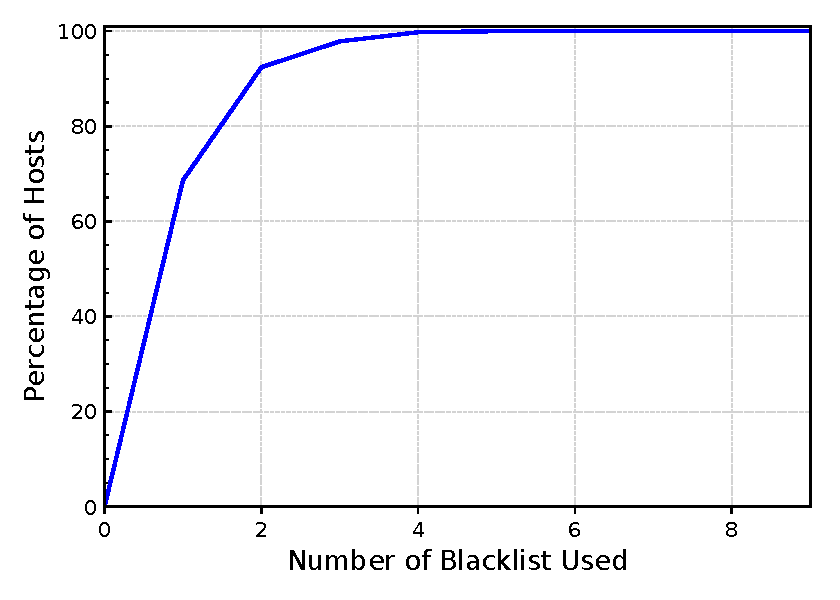
\includegraphics[width=0.8\linewidth]{data_usage/images/perfect_shared_cdf_v2.pdf}
  \caption{CDF of the number of blacklists used by {\reflectors}}
  \label{fig:perfect-shared-cdf}
\end{figure}

\subsection{Multiple Blacklist Use}

For the {\reflectors} using at least one blacklist,
Figure~\ref{fig:perfect-shared-cdf} shows the cumulative distribution
of the number of blacklists they use.  At least for the most popular
public blacklists I study, most use just one.  Over 68.6\% use just
one blacklist, 23.8\% use two or more, and only 7.6\% use three or more.
I find one {\reflector} using six of the nine blacklists -- the most
I see in my study.

For these {\reflectors}, though, there are interesting patterns to the
multiple blacklists used.  Figure~\ref{fig:perfect-heatmap} shows the
use of multiple blacklists with a heatmap.  Each cell shows the fraction of the {\reflectors} using the blacklist in the
   row $R$ that are also using the blacklist in the column $C$: $|R \cap C| / |R|$. Rows and columns
correspond to blacklists, and each cell of the heatmap shows the
fraction of the {\reflectors} using the blacklist in row $R$ that are
also using the blacklist in column $C$.  For example, the first cell
for {\etcompromised} shows that 78\% of the {\reflectors} that use ET
also use the {\spamhausdrop} blacklist.  Diagonal cells are 1.00 since
they show blacklists compared with themselves.

The first cell of the {\spamhausedrop} row indicates that all
{\reflectors} that use {\spamhausedrop} also use {\spamhausdrop}.
Since the eDROP list is an extension of the DROP list, the behavior is
strongly consistent with expectations (and, as such, is also a minor
validation of the methodology).  Moreover, the many significant values
in the first two columns show that {\reflectors} that use any of the
other blacklists very often also use {\spamhausdrop} and eDROP.  These
results underscore the popularity of {\spamhausdrop}, and indicate
that if a {\reflector} blocks traffic using blacklists, it very likely
uses {\spamhausdrop}.

\begin{figure}[t]
  \centering
  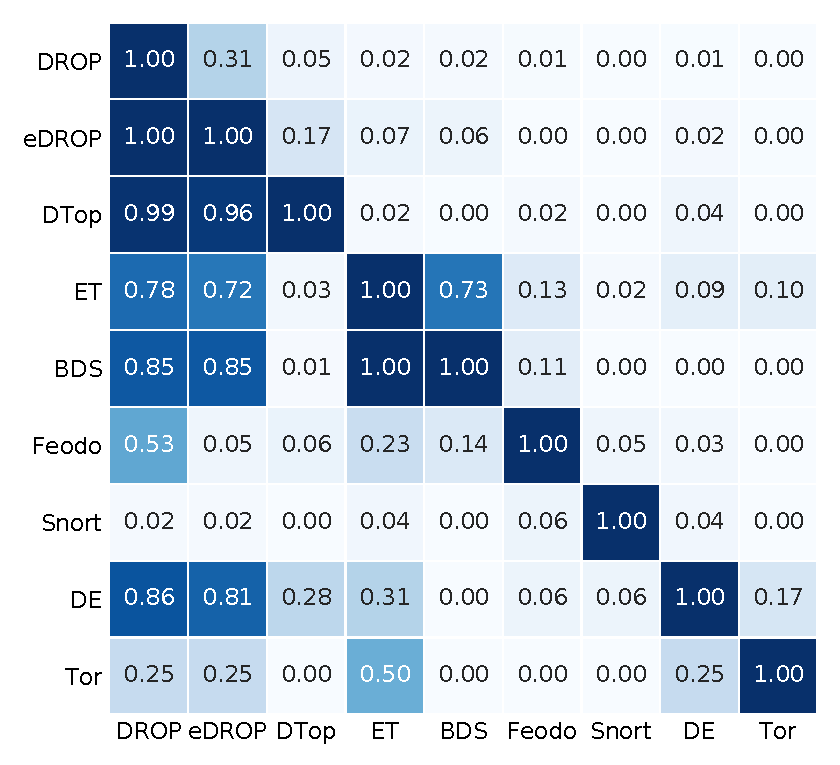
\includegraphics[width=0.85\linewidth]{data_usage/images/perfect_blocking_heatmap.pdf}
  \caption{Pair-wise overlap of {\reflectors} using the different blacklists.}
  \label{fig:perfect-heatmap}
\end{figure}

\subsection{Reflector Update Latency}
\label{sec:latency-analysis}

The objective of IP blacklists is to capture the most up-to-date IPs
associated with malicious activities. As new threats come and go on
the Internet, the content on the lists keeps changing. This dynamic
nature of underlying threats and thus the IPs on the blacklists
underscores the importance of {\reflectors} keeping their blacklists
recent.
%% Thus far, we focused on the stable portion of the blacklist,
%% in order to infer usage.
The goal of our next experiment is to estimate the delay between when
new IPs appear on a blacklist and when reflectors start blocking them.

%% However, to infer update behavior of
%% {\reflectors} we use IPs that are newly added to the blacklist so as
%% to measure how long it takes for {\reflectors} to start blocking the
%% new IPs. We refer this analysis as \textit{latency} analysis.

%% The latency analysis is time sensitive and to get fine granularity
%% we would need to determine the blocking behavior quickly. However,
%% our inference technique is not an instant test. The measurement
%% infrastructure and ethical considerations constrains how quickly
%% we finish the experiment. Typically, the measurement lasts
%% in the order of hours -- allowing us to measure ``latency'' at a
%% day granularity.

%Furthermore, when testing mulitple blacklist IPs against one host, these
%experiments have to be run sequentially, one after another. Otherwise, the
%effects of probing packets on the IP ID field will be mixed together. Also,
%we need to have some gap between each experiment, ensuring different
%experiments will not interfere with each other. All these requirements can
%make one measurement to take hours to finish, making it insufficient to be
%used to reason fine-granularity latency. Therefore, in this experiment we
%focus on day-granularity latency, where we %check how many days do it take
%for each {\reflector} to start blocking newly added IPs %in blacklists.

Because a single pass of the full set of {\reflectors} takes hours, we
examine the blacklist update behavior of {\reflectors} at the
granularity of a day.  For each blacklist we identify newly added IPs
between two consecutive days, and consider only those new IPs that
were not on the blacklist in the prior two weeks.  For this
measurement, the blacklist IPs do not need to be exclusive, but still
need to be routable.  One day after the new IPs appear on a blacklist,
we then test whether the {\reflectors} using that blacklist now block
these IPs, we repeat the experiment daily afterward if necessary.
We also conduct this latency experiment twice to ensure consistent
results(Since {\ettor} is a synthesized list, we did not measure
the update latency regarding this blacklist).

%% After curating this list of blacklist IPs to measure we wait
%% for 24 hours and check if the {\reflectors} we identified in the
%% previous section block these IPs. If no blocking behavior is
%% identified we keep repeating the experiment every day till we see
%% blocking. We repeat this experiment at a later date to ensure
%% consistent results.

%Here we wait for 24 hours because some hosts could update their blacklist
%daily on a fix time (One university we checked update their blacklists every
%day on 6am), then our experiments time might miss the timing.

%% {\dshieldtop},
%% {\etcompromised}, {\bdsatif}, {\bdsatif}, {\feodo}, {\snortfilter},
%% {\blocklistde}, start blocking the newly added IPs on our first measurement
%% indicating that {\reflectors} update their blacklist in a timely manner.

Aside from one outlier, we find that \textit{all} reflectors track
updates to the blacklists. The {\reflectors} that use the six
non-Spamhaus blacklists all update within the one-day period. The
outlier is a group of reflectors using {\spamhausdrop} that stop updating
after late October 2019 (We observed this by testing with the newly added IPs
in {\spamhausdrop} in the past), all the other {\reflectors} that block
{\spamhausdrop} update within one-day period. After investigating, we found that
all these outlier {\reflectors} are located in one organization (a hosting
provider). We suspect this organization stops updating their list after that
October.

For {\spamhausedrop}, it hasn't added new IPs since Dec 17, 2019 as of Feb 14,
2020. We tested all the corresponding {\reflectors} with the newly added IPs
in {\spamhausedrop} back on Dec 17, 2019 and before, and found all the
{\reflectors} are update to date.

%% Thus, in this case we construct lists of ``newly added IPs'' of two
%% list in the past, and check if the {\reflectors} are up to date on
%% these lists.  We find that all {\reflectors} that use {\spamhausedrop}
%% block the set of newly added IPs on December 17th, indicating that
%% these reflectors are up to date. However, in the case of
%% {\spamhausdrop} while most {\reflectors} block the latest newly added
%% IPs, for 2,772 {\reflectors} we find that we need to go before Nov
%% 2019 to find ``newly added IPs'' that are blocked. Mapping the
%% {\reflectors} IPs to an AS and then to an organization using the CAIDA
%% AS to Organization~\cite{caida_as_org} dataset we find that all 2,772
%% {\reflectors} belong to one organization. We suspect this organization
%% included the {\spamhausdrop} on late October 2019 and never updated
%% the list afterwards.

% and strongly
%indicates the use of network level blocking using {\spamhausdrop} by the
%organization.

%, it is a little bit challenging since
%these two lists do not update frequently---only a few times per mont. Worse,
%these new IPs are often unroutable, making them unsuitable for our measurement.
%Therefore, we calculate the newly added IPs in these two lists in the past,
%using the data we collected, and test against the corresponding {\reflectors}.
%We found that all {\reflectors} that use {\spamhausedrop} are blocking the
%latest IPs(added on Dec 17th). While for {\spamhausdrop}, there are 2,772
%{\reflectors} that only blocks IPs that are added earlier than Nov 2019, and
%all the other {\reflectors} are blocking the latest IPs(added on Feb 4th 2020).
%And all these IPs are from the one organization. We suspect this organization
%included the {\spamhausdrop} on late October 2019 and never updated their list.

\subsection{Validation}

We are able to infer the use of blacklists for various hosts from our
measurement. Ideally, we would also want to validate our findings.
After checking the organizations where our {\reflectors} are from, we
reached out to 2 universities that we conclude are using blacklists.
We got the ground truth regarding the exact blacklists they are using, and
successfully validated our findings. More specifically, University $A$
confirmed our findings that they use \bdsatif, \etcompromised,
\spamhausdrop\ and \spamhausedrop. University $B$ confirmed our finding that
they use \spamhausdrop\ and \spamhausedrop.

%For the Tor list blocking, we check the reverse DNS of the {\reflectors},
%and for the ones that we can find the reverse DNS record, we access the website
%from a normal browser and at the same time, from a TOR browser. We observed
%that for all these reflectors, we can access them from a normal browser, but can not
%establish a connection from the Tor browser, proving that they are
%blocking connections from Tor.


\section{Partial Blocking}
\label{sec:partial-blocking}

%% In Section~\ref{sec:perfect-blocking}, we looked into {\reflectors} that
%% consistently block all blacklist IPs sampled for a blacklist. We further
%% confirm this by re-running the measurement three times with three different
%% set of blacklist IPs sampled from the blacklist at different times. However,
%% our measurement also discovers blocking behavior that is not ``perfect''.
%% Every time we sample blacklist IPs and test, many {\reflectors} only block
%% some of the IPs we sampled, while leaving the rest of IPs unblocked. We refer
%% to these cases as \textit{partial blocking}. In this section, we dive deeper
%% into these cases of partial blocking. Specifically, we look at different reasons
%% one may see partial blocking and then look in more detail at {\reflectors}
%% that show consistent, and significant partial blocking.

When performing our experimental runs we noticed that a small
percentage of reflectors consistently blocked a significant subset of
blacklist IPs, but not all, in \textit{every experiment}.
This consistency suggests that, while the
{\reflector} may not use the exact blacklist, there is a large overlap
between the blacklist and the blocking policy of the {\reflector}.  We
refer to such reflectors as exhibiting \textit{significant partial blocking}
behavior.  Figure~\ref{fig:reflector-breakdown} shows these reflectors
are just 0.4\% of all reflectors that we tested, but they still
correspond to 21\% of the number of reflectors that perfectly block at
least one blacklist and therefore motivate further investigation.  As
a result, in this section we characterize this partial blocking
behavior in more detail.

%% Therefore, if a {\reflector} only blocks a small portion of the IPs we
%% sampled from a blacklist, it could not give us much insight about the
%% host's behavior regarding that blacklist.

%% However, we observe that many of these {\reflectors} show partial
%% blocking behavior consistently: Every time we test with a certain
%% blacklist, they always block a significant portion of the IPs we
%% sampled from that list.

%% However, before we dive deeper into these {\reflectors} we briefly touch upon
%% geo-blocking -- a significant contributor to partial blocking and how we try and
%% reduce the effects that geo-blocking may have on our results.
%\textcolor{red}{Show the table about the breakdown between >75\% and >50\%}.

\subsection{Geo-Blocking}
\label{sec:geo-blocking}

%% Geo-blocking is the case where the {\reflector} blocks all the traffic from a
%% certain country. Some sites apply this blocking either for policy reason
%% (e.g. block GDPR countries~\cite{bbcnews}.), or for security reasons (e.g.
%% block countries where recent attacks originated from, like Russia or China).
%% Although during blacklist IP sampling, we go the extra mile to increase the
%% geo diversity of IPs, we might still end up with sampled IPs largely from a
%% few countries. Primarily, this is because the blacklist itself can have a
%% disproportionate amount of IPs from only a few countries. For example,
%% {\dshieldtop} on Jan. 25th had over 50\% of its IPs coming from Netherlands.
%% If a host blocks traffic from Netherlands, then we would miss conclude that
%% host is partially blocking {\dshieldtop}.

%% To eliminate the effects of geo-blocking, we conducted an additional
%% experiment to identify the geo-blocking hosts among our {\reflectors}. For
%% each country the blacklist IPs had covered, we randomly select 20 IPs from
%% that country, and test against all {\reflectors}, using the same IP ID
%% technique, to identify if the hosts that are blocking these IPs. Here we
%% acquire IP address prefixes of each country from 4 location services:
%% MaxMind~\cite{maxmind}, IP2Location~\cite{ip2location}, IPDeny~\cite{ipdeny}
%% and IPIP.net~\cite{ipip}, and we only sample IPs from the intersection of the
%% prefixes provided by each service. Put differently, for each country we test,
%% we only sample from the IPs where all 4 location services are agree they are
%% from that country. We further make sure the sampled IPs are not overlapped
%% with any of the blacklists we have, and they are BGP routable. We tested 20
%% countries in total, from big countries like Russia and China, to small island
%% countries like Singapore and Seychelles.

%% In total, we identify 677 {\reflectors} that at least block one country we
%% tested, and 473 {\reflectors} that block at least two countries. 549
%% {\reflectors} block IPs from China, making it the most popular target of
%% geo-blocking in our collection. Russia is the second most blocked country,
%% where we found 414 hosts blocking Russian IPs, followed by Hong Kong and
%% Vietnam, for which there are 196 and 193 {\reflectors} blocking their IPs
%% respectively. European countries like Belgium, Netherlands and France also
%% have over 60 hosts blocking them.

%% Note that what we discovered here is network layer geo-blocking, and there
%% can be other forms of geo-blocking, like application layer blocking (e.g.
%% HTTP 403 Forbidden). We do not try to comprehensively cover all possible
%% geo-blocking cases since this experiment was only to help us identify the
%% potential side-effects of geo-blocking in our experiment, so we could better
%% distinguish the blacklist related blocking behavior in our experiment.

%% One potential cause of partial blocking is geo-blocking.

Geo-blocking is one type of blocking we identified that contributes to
this partial blocking.  A {\reflector} using geo-blocking will
drop all traffic from a particular country.  Organizations typically
use geo-blocking either for policy reason (e.g., block GDPR
countries~\cite{bbcnews}), or for security reasons (e.g., block
countries that are sources of attacks, such as Russia or China).  If a
reflector uses geo-blocking, we will observe it blocking IPs on a
blacklist if those IPs happen to be located in a blocked country.  Although
we take extra efforts to increase the geo diversity when sampling IPs(Section~\ref{sec:methtarg}),
this kind of overlap can still be exacerbated if a blacklist happens to have
concentrations of IPs from particular countries.  For example,
{\dshieldtop} on January 25, 2020 had over 50\% of its IPs geo-located
in the Netherlands.  If a reflector blocks traffic from the
Netherlands, then we would observe that the reflector is partially
blocking {\dshieldtop}.

%% Recall that Although during blacklist IP sampling, we go the extra
%% mile to increase the geo diversity of IPs, we might still end up with
%% sampled IPs largely from a few countries. Primarily, this is because
%% the blacklist itself can have a disproportionate amount of IPs from
%% only a few countries.

To identify whether a {\reflector} uses geo-blocking, we test whether
the {\reflector} consistently blocks a set of IPs from a particular
country.  For all countries related to blacklist IPs that we test, we
first enumerate the IP address prefixes for those countries using four
IP-based location services: MaxMind~\cite{maxmind},
IP2Location~\cite{ip2location}, IPDeny~\cite{ipdeny}, and
IPIP.net~\cite{ipip}.  For each country, we then randomly select 20 IP
addresses from those prefixes such that: (1) all four location
services agree on the country label for the IPs, (2) the IPs do not
appear on a blacklist, and (3) the IPs are BGP routable.  Then for all
{\reflectors}, we test whether it blocks all of the randomly-chosen
IPs for each country.  If it does, then we conclude that it uses
geo-blocking.

We tested our {\reflectors} against 20 countries in total, ranging
from large countries like Russia and China to small island countries
like Singapore and Seychelles.  Overall, only a small number of
{\reflectors}, 614 (0.28\%), block at least one country, and 432 block
at least two.  China is blocked most often, with 501 of the 614
{\reflectors} blocking random IPs in China.  Russia is second at 376,
followed by Hong Kong (177) and Vietnam (175).  European countries
including Belgium, Netherlands, and France also have over 60
{\reflectors} blocking them.

Note that our methodology identifies geo-blocking at the network
layer.  Other forms of geo-blocking exist, such as application-layer
blocking (e.g., HTTP 403 Forbidden).  We do not explore all possible
geo-blocking mechanisms since our goal was to identify {\reflectors}
using geo-blocking at the network layer.

%% \noteby{GV}{Thinking about it more, if we had more time we could turn
%%   geo-blocking into a result instead of treating it as error.  The
%%   challenge with fitting it into the current framing is that it is not
%%   always significant partial blocking.}

%% , as they could introduce noise
%% when determining network-level blocking based upon blacklists.

\subsection{Significant Partial Blocking}

\begin{table}[t]
\centering
\small
%\begin{adjustbox}{width=\columnwidth}
\begin{tabular}{l r r r | r r r }
 \toprule
 \textbf{}           &\multicolumn{3}{c}{\textbf{Blocked over 75\%}}    &\multicolumn{3}{c}{\textbf{Blocked over 50\%}} \\
 \textbf{Blacklist}  &\textbf{Hosts}   &\textbf{/24s}   &\textbf{ASes}  &\textbf{Hosts}   &\textbf{/24s}   &\textbf{ASes} \\
 \midrule
 DROP      & 28      & 18     & 3   &  23      & 21    & 3\\
 eDROP     & 96      & 60     & 32  &  49      & 27    & 18\\
 DTop        & 157     & 66     & 19  &  319     & 165   & 72\\
 ET     & 13      & 7      & 6   &  31      & 19    & 17\\
 BDS           & 8       & 5      & 5   &  7       & 7     & 7\\
 Feodo             & 65      & 30     & 19  &  23      & 17    & 15\\
 Snort       & 11      & 9      & 7   &  34      & 20    & 17\\
 DE       & 148     & 38     & 1   &  13      & 11    & 4\\
 Tor             & 63      & 35     & 26  &  31      & 19    & 16\\
 %% {\spamhausdrop}      & 28      & 18     & 3   &  23      & 21    & 3\\
 %% {\spamhausedrop}     & 96      & 60     & 32  &  49      & 27    & 18\\
 %% {\dshieldtop}        & 157     & 66     & 19  &  319     & 165   & 72\\
 %% {\etcompromised}     & 13      & 7      & 6   &  31      & 19    & 17\\
 %% {\bdsatif}           & 8       & 5      & 5   &  7       & 7     & 7\\
 %% {\feodo}             & 65      & 30     & 19  &  23      & 17    & 15\\
 %% {\snortfilter}       & 11      & 9      & 7   &  34      & 20    & 17\\
 %% {\blocklistde}       & 148     & 38     & 1   &  13      & 11    & 4\\
 %% {\ettor}             & 63      & 35     & 26  &  31      & 19    & 16\\
 \midrule
 \textbf{Total}              & 492     & 207    & 71  & 459      & 257   & 108\\
 \bottomrule
\end{tabular}
%\end{adjustbox}
\caption{Number of reflectors exhibiting significant partial blocking on each blacklist.}
\label{tab:partial-blocking-reflectors}
\end{table}

%\noteby{GV}{At what point in the workflow are geo-blocking reflectors
%  removed?}

%% Recall that we selected all {\reflectors} exclusively within the US to
%% minimize blocking behavior caused by censorship
%% (Section~\ref{sec:methrefl}).

In addition to geo-blocking, there are reasons why a {\reflector} may
block a blacklist IP that is not due to the reflector using that
blacklist.  A host may have internal policies that deny access from
some network providers, or network administrators may add IPs into
their firewall on an ad-hoc basis based on an organization's internal
strategies or policies.  These alternate blocking behaviors could
overlap with the blacklist IPs we sampled, leading to partial blocking
behavior in our results.

%% We go through all partial blocking we observed, and remove the ones
%% that caused by geo-blocking.

Having identified reflectors using geo-blocking, we remove these
reflectors from further consideration.  We then calculate two groups of
{\reflectors}: for each blacklist, we identify {\reflectors} that
partially block over 75\% of our sampled IPs \textit{every time} we
test them, and another group where they partially block over 50\% of
our sampled IPs.
%We exclude the cases where we fail to conclude the blocking behavior of a
%few {\reflectors} and blacklist IP pairs (after 15 trials)
%\noteby{GV}{Not clear on this?}.

%Every time we test, we sample IPs from the exclusive part of that blacklist,
%where we check against over 100 public IP blacklist (including some obsolete
%ones). Therefore,

For each blacklist, Table~\ref{tab:partial-blocking-reflectors}
summarizes the number of {\reflectors} that fall into each category.
If a {\reflector} is blocking more than 75\% of our sampled IPs every
time, it is plausible that the {\reflector} is using a source that is
very similar to the blacklist we tested.  For instance, there could be
other blacklists where the data collection methodology is similar to
the method used by the public blacklists in our study.  Previous work
has shown that commercial products can aggregate data from public
blacklists, and that they potentially conduct post-processing to
eliminate some content~\cite{li2019reading}.

We suspect that the partial blocking behavior in
Table~\ref{tab:partial-blocking-reflectors} likely results from such
cases.  In particular, the number of {\reflectors} that are partial
blocking {\dshieldtop} is relatively high compared with other
blacklists---it covers over 30\% of all {\reflectors} in the first
group and over 69\% in the second group, suggesting that this list may
be relatively frequently included into other lists.

%% Looking into the organizations related to these partial blocking hosts
%% (Section~\ref{sec:perfect-blocking}), {\feodo} is again covered by the
%% most diverse set of organizations, showing its popularity among
%% different sectors.  \noteby{GV}{Keep in mind that the next section
%%   claims that we cannot map to organizations...}

%% Overall, though, only a small number of {\reflectors} show significant
%% partial blocking, which is consistent with the finding in the previous
%% section.

%% (Less is More)
%% One interesting fact is that there are 253 {\reflectors} from
%% the two partial blocking groups overlap with the {\reflectors} we
%% identified previously that use a blacklist, which is because some
%% {\reflectors} use one blacklist but only partially block another.

\section{Beyond Our Blacklists}
\label{sec:large-scale}

%In this section we analyze how fast does different network update their blocking policy.
%So far the goal of our measurement was to infer if a {\reflector} uses a
%specific blacklist to block traffic. While this informs our view of the usage
%of specific blacklists it does not inform our broader perspective on the
%usage of threat intelligence at large. Essentially, in this section we would
%like to see if any of our {\reflectors} use any blacklist, or implement any
%security features that involves IP-based traffic blocking.

%During our measurement, we looked at over 100 public IP blacklists, but there
%is a wide selection of commercial blacklists that we cannot cover. In order
%to look at the blocking behavior from a wider lens, we would like to test
%blacklist IPs that are shared by as many products as possible. Of course,
%there is no concrete way to identify these IPs, so we try to use some
%heuristic to increase the likelihood that the IPs selected are also covered
%by other blacklists.

%In order to accomplish this, we still sample IPs from the top 9 blacklist we
%identified, but instead of selecting exclusive IPs, we sample from the
%\textit{nonexclusive} portion of each blacklists, so that these IPs are
%shared with at least one more blacklist. We further reduce the candidate pool
%by only keeping the IPs that have stayed in the blacklist for at least 3
%weeks. Being ``shared'' and ``stable'' are the heuristics we use to increase
%the chances that these IPs are also shared with many other blacklists. We
%then drop the IPs that are not routable or are from the {\reflector} AS.
%Finally, we randomly sample 80 IPs from the remaining IPs for our experiment.
%We test these IPs against all our {\reflectors} to identify blocking
%behaviors. To be conservative, we conduct this experiment twice and use two
%different set of randomly selected 80 IPs. Additionally, each time we also
%include a control group, where we randomly select 80 IPs from
%\textcolor{red}{Explain how control group come.}

\begin{figure}[t]
\centering
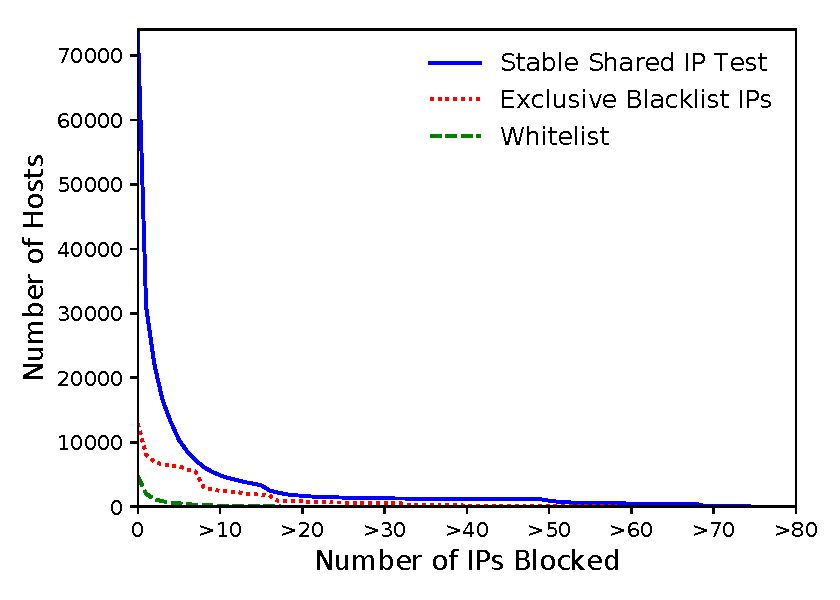
\includegraphics[width=1.0\columnwidth]{images/large_scale_rcdf_v2.pdf}
\caption{Number of {\reflectors} ($y$-axis) that block at least
  some number of blacklist IPs ($x$-axis).  5,412 reflectors,
  for instance, block 10 or more ``Shared'' IPs.}
\label{fig:large_scale_rcdf}
\end{figure}


Previously we chose blacklist IPs that were exclusive to each
blacklist, effectively creating a set of IPs that served as a
signature for that blacklist. But as we can see from Figure~\ref{fig:reflector-breakdown},
there are over 20\% of {\reflectors} that blocked at least one
blacklist IP during one of the three experiments, and we do not
have a clear explanation. One possible case is that the blacklist IPs
we sampled happen to overlap with some commercial blacklists we
do not know, and those lists are more widely used. To check this
possibility, we change our blacklist IP sampling criteria and conduct
a new experiment.

Now our goal is the opposite: we want
to choose among common, or shared, IPs that appear on multiple
blacklists.  As added caution, we also focus on shared IPs that are
the most stable, appearing on the blacklists for at least three weeks.
Our goal is to bias selecting blacklist IPs that are so egregiously
suspicious that not only do they appear on multiple of our public
blacklists for a long period of time, but as a result they also likely
appear on other public and commercial blacklists that we do not have
access to.

% \noteby{GV}{Opportunity for an analogy here.}

For this experiment we randomly selected 80 blacklist IPs that appear
on more than one blacklist and, as with previous experiments, that are
routable and AS disjoint.  We refer to this set as the ``Shared''
blacklist IPs.  For comparison, we also randomly selected a set of 80
blacklist IPs from our previous experiment, the ones that are
exclusive to one blacklist (``Exclusive''), and a random set of 80 IPs
as a whitelist set (``Whitelist''), again with the routable and AS disjoint
criteria. Here the whitelist is constructed by randomly sampling IPs
from top 10,000 most visited IPs among all the network traffic in our own
organization in one day (an education institute of over 30K students
and faculty).


%% This is showed as the green dash line in Figure~\ref{fig:large_scale_rcdf}.

For each of these sets of 80 blacklist IPs,
Figure~\ref{fig:large_scale_rcdf} shows how many {\reflectors} block
the same number of IPs as a distribution over the number of blacklist
IPs blocked.  (We evaluated multiple random sets of shared blacklist
IPs to see whether the random selections introduced noticeable
variance.  Since the results were very consistent across the different
random sets, for clarity we just show results for one of them.)  For
example, for ``Exclusive'' blacklist IPs only 2,649 {\reflectors}
block 10 or more IPs.  In contrast, for ``Shared'' blacklist IPs that
appear on more than one blacklist, far more {\reflectors} block them.
Over 73K {\reflectors} block at least one IP from the shared set, and
5,412 {\reflectors} block 10 or more IPs.  In contrast, for the
whitelist set, there are only 202 {\reflectors} that block 10 or more
whitelist IPs(we checked these whitelist IPs and found the most blocked
ones are from Cloudflare, which is a popular CDN network but
known to associate with malicious activities).
These results suggest that the number of Internet
hosts that potentially use security-related traffic blocking is much
larger than just the ones that use the public blacklists we study.

%% \noteby{GV}{Since shared 1 and 2 essentially overlap, we can just show
%%   one on the graph.  I added the footnote to convey that we did this
%%   more than once for added reassurance.}\noteby{VL}{I still feel it
%%   is a little bit weird if we do not show both result in the graph, because in
%%   the following we say we use top 12 IPs in \textbf{two} experiments}.

%% Uses a larger font size
\begin{table}[t]
\centering
\small
\begin{tabular}{r  r  r  r}
 \toprule
                         & \multicolumn{3}{c}{\textbf{Granularity}} \\
 \textbf{Blacklist IP}   & \textbf{IP}  & \textbf{/24}   & \textbf{AS}\\
 \midrule
 178.73.215.171             & 25,749                 & 175        & 210     \\
 185.176.27.98              & 15,560                 & 5,598      & 1,690   \\
 185.175.93.103             & 13,550                 & 1,155      & 1,224   \\
 92.63.194.115              & 11,889                 & 2,028      & 1,442   \\
 176.10.99.200              & 9,049                  & 466        & 238     \\
 185.156.73.54              & 8,863                  & 1,623      & 5,441   \\
 80.67.223.41               & 6,689                  & 624       & 624      \\
 176.100.109.3              & 4,871                  & 553       & 610      \\
 171.25.193.25              & 4,468                  & 212       & 148      \\
 216.239.90.19              & 4,421                  & 56        & 39       \\
 185.220.102.8              & 4,297                  & 273       & 273      \\
 62.210.37.82               & 4,058                  & 528       & 300      \\
 \bottomrule
\end{tabular}
\caption{Blocking behavior of reflectors with the top 12 most-blocked
  blacklist IPs.  The second column shows the number of {\reflectors}
  that block the particular IP, the third column shows the
  \textit{maximum} number of {\reflectors} that block IPs from the
  same /24, and the last column shows the maximum number of
  {\reflectors} that block IPs sampled from the same AS.}
\label{tab:super-malicious-ips}
\end{table}


% (probably should have the %s in separate columns for more convenient column space control)
\begin{table*}[t]
	\centering
	\small
	\begin{tabular}{l|rr|r|r} \toprule
		\multicolumn{1}{c}{\textbf{}} & \multicolumn{2}{c}{\textbf{Consistent}}                                                      & \multicolumn{1}{c}{\textbf{Almost Consistent}} & \multicolumn{1}{c}{\textbf{Inconsistent}}      \\
		\textbf{Blacklist}            & \multicolumn{1}{c}{\textbf{No Blocking (\%)}} & \multicolumn{1}{c|}{\textbf{Consistent (\%)}} & \multicolumn{1}{c|}{\textbf{Off By One (\%)}}   & \multicolumn{1}{c}{\textbf{Inconsistent (\%)}} \\
\midrule
{\bdsatif} & 35,540 \hspace*{2pt} (88.19\%) & 398 \hspace*{2pt} (0.99\%) & 2,332 \hspace*{2pt} (5.79\%) & 2,030 \hspace*{2pt} (5.03\%) \\
{\blocklistde} & 40,228 \hspace*{2pt} (99.82\%) & 24 \hspace*{2pt} (0.06\%) & 13 \hspace*{2pt} (0.03\%) & 35 \hspace*{2pt} (0.09\%) \\
{\dshieldtop} & 39,603 \hspace*{2pt} (98.27\%) & 393 \hspace*{2pt} (0.98\%) & 138 \hspace*{2pt} (0.34\%) & 166 \hspace*{2pt} (0.41\%) \\
{\etcompromised} & 39,535 \hspace*{2pt} (98.10\%) & 298 \hspace*{2pt} (0.74\%) & 102 \hspace*{2pt} (0.25\%) & 365 \hspace*{2pt} (0.91\%) \\
{\feodo} & 39,943 \hspace*{2pt} (99.11\%) & 195 \hspace*{2pt} (0.48\%) & 42 \hspace*{2pt} (0.10\%) & 120 \hspace*{2pt} (0.31\%) \\
{\snortfilter} & 39,830 \hspace*{2pt} (98.83\%) & 250 \hspace*{2pt} (0.62\%) & 88 \hspace*{2pt} (0.22\%) & 132 \hspace*{2pt} (0.33\%) \\
{\spamhausdrop} & 39,320 \hspace*{2pt} (97.57\%) & 750 \hspace*{2pt} (1.86\%) & 30 \hspace*{2pt} (0.07\%) & 200 \hspace*{2pt} (0.50\%) \\
{\spamhausedrop} & 39,792 \hspace*{2pt} (98.73\%) & 349 \hspace*{2pt} (0.87\%) & 36 \hspace*{2pt} (0.09\%) & 123 \hspace*{2pt} (0.31\%) \\
{\ettor} & 40,000 \hspace*{2pt} (99.25\%) & 165 \hspace*{2pt} (0.41\%) & 43 \hspace*{2pt} (0.11\%) & 92 \hspace*{2pt} (0.23\%) \\
\midrule
\textbf{Overall} & 353,791 \hspace*{2pt} (97.54\%) & 2,822 \hspace*{2pt} (0.78\%) & 2,824 \hspace*{2pt} (0.78\%) & 3,263 \hspace*{2pt} (0.90\%) \\
\midrule
\textbf{Control Group} & 40,255 \hspace*{2pt} (99.89\%)	& 3 \hspace*{2pt} (0.01\%) & 37 \hspace*{2pt} (0.09\%) & 5 \hspace*{2pt} (0.01\%) \\
\bottomrule
	\end{tabular}
	\caption{The blocking consistency of the reflectors in /24 prefixes with more than one reflector.  Multiple reflectors in most /24 prefixes do not block, and as such are consistent.  But when multiple reflectors in /24 prefixes do block, there is substantial inconsistency.  }
	\label{tab:consistency-breakdown}
\end{table*}

Of course, it is possible that this more extensive blocking behavior
is not a result of security-related blocking, but rather because of
other blocking policies such as geo-blocking.  One notable difference,
though, is that security-based traffic blocking usually targets
individual IPs, whereas other policy-driven blocking can target a
specific network or subnet.  As another experiment, we check whether
the blocking we observed indeed targets individual IPs, or instead
larger network blocks.  We select the top 12 IPs where they have
the most amount of {\reflectors} blocking them in the previous test.
For each of these blacklist IPs, we randomly sample
another three IPs from the same /24, and randomly sample another four
IPs from the same AS.  For all of these IPs, we then measure how many
{\reflectors} block each of them.

%% (Original version)
%%
%% \begin{table}[t]
%% \centering
%% \footnotesize
%% \begin{tabular}{r | r | r | r}
%%  \toprule
%%  \textbf{Blacklist IP}   & \textbf{Blocking IP}  & \textbf{Blocking /24}   & \textbf{Blocking AS}\\
%%  \midrule
%%  178.73.215.171             & 25,749                 & 175        & 210     \\
%%  185.176.27.98              & 15,560                 & 5,598      & 1,690   \\
%%  185.175.93.103             & 13,550                 & 1,155      & 1,224   \\
%%  92.63.194.115              & 11,889                 & 2,028      & 1,442   \\
%%  176.10.99.200              & 9,049                  & 466        & 238     \\
%%  185.156.73.54              & 8,863                  & 1,623      & 5,441   \\
%%  80.67.223.41               & 6,689                  & 624       & 624      \\
%%  176.100.109.3              & 4,871                  & 553       & 610      \\
%%  171.25.193.25              & 4,468                  & 212       & 148      \\
%%  216.239.90.19              & 4,421                  & 56        & 39       \\
%%  185.220.102.8              & 4,297                  & 273       & 273      \\
%%  62.210.37.82               & 4,058                  & 528       & 300      \\
%%  \bottomrule
%% \end{tabular}
%% \caption{Blocking behavior of reflectors with the top 12 most-blocked
%%   blacklist IPs.  The second column shows the number of {\reflectors}
%%   that block the particular IP, the third column shows the
%%   \textit{maximum} number of {\reflectors} that block IPs from the
%%   same /24, and the last column shows the maximum number of
%%   {\reflectors} that block IPs sampled from the same AS.}
%% \label{tab:super-malicious-ips}
%% \end{table}


Table~\ref{tab:super-malicious-ips} shows the number of {\reflectors}
that block the top 12 blacklist IPs, the random IPs from the same
/24 as the blacklist IPs, and the random IPs from the same AS (For the
/24 test and AS test, we listed the maximum number of {\reflectors} that
block IPs in two tests). These
results confirm that {\reflectors} exhibit blocking behavior targeting
specific IPs rather than larger network blocks.  Indeed, searching the
Web based on these blacklist IPs returns reports linking these IPs to
a range of malicious activities, including massive port scanning,
brute-force login attempts, and sending spam. That said, although we do
not know the exact feeds these hosts are using, our results suggest
that security-related network blocking is prevalent even among hosts
such as these reflectors.

\section{Blocking Consistency}
\label{sec:consistency}
% TODO: Location of the Table! :(
% GEOFF: Link to the breakdown by AS Type
% https://docs.google.com/spreadsheets/d/1QAWr1qb01reJVAmhvl-ukOJjDl5E_1kr_uIQrAOwWyo/edit#gid=691238820
%
%% \begin{table*}[t]
%% 	\centering
%% 	\small
%% 	\begin{tabular}{l|rr|r|r} \toprule
%% 		\multicolumn{1}{c}{\textbf{}} & \multicolumn{2}{c}{\textbf{Consistent}}                                                      & \multicolumn{1}{c}{\textbf{Almost Consistent}} & \multicolumn{1}{c}{\textbf{Inconsistent}}      \\
%% 		\textbf{Blacklist}            & \multicolumn{1}{c}{\textbf{No Blocking (\%)}} & \multicolumn{1}{c}{\textbf{Consistent (\%)}} & \multicolumn{1}{c}{\textbf{Off By One (\%)}}   & \multicolumn{1}{c}{\textbf{Inconsistent (\%)}} \\ \hline
%% 		\textbf{\bdsatif}              & 35540 (88.19\%)                               & 398 (0.99\%)                                 & 2332 (5.79\%)                                  & 2030 (5.03\%)                                  \\
%% 		\textbf{\blocklistde}          & 40228 (99.82\%)                               & 24 (0.06\%)                                  & 13 (0.03\%)                                    & 35 (0.09\%)                                    \\
%% 		\textbf{\dshieldtop}           & 39603 (98.27\%)                               & 393 (0.98\%)                                 & 138 (0.34\%)                                   & 166 (0.41\%)                                   \\
%% 		\textbf{\etcompromised}        & 39535 (98.10\%)                               & 298 (0.74\%)                                 & 102 (0.25\%)                                   & 365 (0.91\%)                                   \\
%% 		\textbf{\feodo}                & 39943 (99.11\%)                               & 195 (0.48\%)                                 & 42 (0.10\%)                                    & 120 (0.31\%)                                   \\
%% 		\textbf{\snortfilter}          & 39830 (98.83\%)                               & 250 (0.62\%)                                 & 88 (0.22\%)                                    & 132 (0.33\%)                                   \\
%% 		\textbf{\spamhausdrop}         & 39320 (97.57\%)                               & 750 (1.86\%)                                 & 30 (0.07\%)                                    & 200 (0.50\%)                                   \\
%% 		\textbf{\spamhausedrop}        & 39792 (98.73\%)                               & 349 (0.87\%)                                 & 36 (0.09\%)                                    & 123 (0.31\%)                                   \\
%% 		\textbf{\ettor}                & 40000 (99.25\%)                               & 165 (0.41\%)                                 & 43 (0.11\%)                                    & 92 (0.23\%)                                    \\
%% 		\midrule
%% 		\textbf{Overall} 			   & 353791 (97.54\%)   & 2822	(0.78\%) & 2824 (0.78\%) & 3263 (0.90\%) \\
%% 		\midrule
%% 		\textbf{Control Group}  	   & 40255  (99.89\%)	& 3	(0.01\%)	& 37 (0.09\%)	 & 5 (0.01\%)	   \\
%% 		\bottomrule
%% 	\end{tabular}
%% 	\caption{Consistency Breakdown}
%% 	\label{tab:consistency-breakdown}
%% \end{table*}

As a final analysis, we explore the consistency of reflector blocking
behavior at a coarser granularity.  A common use case of blacklists is
at the granularity of an organization, often via some kind of network
appliance.  In such a scenario, we would expect the blocking behavior
of {\reflectors} to be consistent across an organization: if one
{\reflector} blocks a blacklist IP, then other {\reflectors} in the
same organization should also block it.

Ideally we would like to map reflectors to organizations to answer
this question.  However, mapping an IP to an organization is a
challenging problem, particularly with the increasing use of WHOIS
anonymization.  Instead, we use the common, more tractable technique
of aggregating reflectors by their /24 prefix.  As a result, in this
section we answer a methodological question: If we aggregate
reflectors by their /24 prefix, do the aggregated reflectors exhibit
consistent blocking behavior?  Is the /24 prefix aggregation a useful
proxy for expected consistent blocking by organizations?

%% However, mapping an IP to an organization is a
%% challenging problem, particularly with the increasing use of WHOIS
%% anonymization.  Further, multiple ``organizations'' could potentially
%% map to a single AS, as with transit and access ASes. Thus, we use the
%% common method of assuming hosts on the same /24 prefix are part of the
%% same network and, as such, the same organization.

%% Specifically, for each /24 with more than one {\reflector}, we check
%% if the {\reflectors} block the exact same set of sampled blacklist IPs.

%\subsection{Consistency Methodology}

Our data set has 134,370 {\reflectors} that are part of /24s with more
than one {\reflector}.  For each blacklist, we categorize the blocking
behavior of multiple {\reflectors} in the same /24 into one of three
categories: \textit{consistent}, \textit{almost consistent}, and
\textit{inconsistent}.  We define a /24 to be ``consistent'' for a
blacklist if \textit{all} the individual {\reflectors} in that /24
block the \textit{exact same} blacklist IPs.
%
A /24 is ``almost consistent'' if the blocking behavior of the
{\reflectors} in a /24 differs only by one IP. For example, a /24 is
``almost consistent'' if it has four {\reflectors}, three of which
block the same 21 IPs from a blacklist, and the fourth {\reflector}
blocks 20 out the same 21 IPs.
%% since if we had tried more than 15 times we could have potentially
%% found them to be consistent.
%
Finally, we consider all other /24s ``inconsistent''.

%% any /24 that does not fall into the aforementioned two categories,
%% we consider them as ``inconsistent''.

%there is the case of missed blacklist IPs -- blacklist IPs for which we could
%not get a good signal for blocking behavior. In the specific instance, where
%the sum of ``perfect'' and ``missed'' blacklist IPs is exactly the same for
%all individual {\reflectors} in a /24 we carve out that /24 as unknown since
%had we persisted beyond 15 tries we could have found it as consistent.

%\subsection{Consistency Results}

Using these definitions, Table~\ref{tab:consistency-breakdown} shows
the consistency results for all the /24s that have more than one
{\reflector}.  The results are dominated by /24s that do not show any
blocking behavior.  We consider such /24s consistent since all the
hosts under these /24s block the same number (zero) of blacklist IPs,
but these cases also do not provide much insight.

Excluding the ``no blocking'' cases, then in the presence of any
blocking, consistency of blocking behavior at a /24 granularity is far
from guaranteed.  As discussed in Section~\ref{subsec:fpfn_analysis},
our measurement technique has very low false positive and false
negative rates.  Measurement error can potentially explain some
``almost consistent'' cases and perhaps some ``inconsistent'' cases,
too.  However, the consistency results for the control group,
comprised of 20 randomly sampled US IPs
(Section~\ref{sec:perfect-blocking}), shows that the potential effect
of measurement error on consistency is small.  In other words, the
inconsistent cases do indeed demonstrate different blocking behavior
among hosts within the same /24.

One situation that could lead to inconsistent blocking behavior within
a /24 is when the network belongs to a cloud or hosting provider, and
the IPs within the same /24 are used by distinct entities.  For
instance, when manually examining the inconsistent /24s for {\bdsatif}
(which has the highest inconsistency), we found more than 60\% of
these /24s belong to cloud or hosting providers.  Another situation
leading to inconsistent block behavior is when a /24 belongs to an ISP
which sub-allocates IP addresses to different customers.

In summary, our results indicate that we cannot assume consistent
blocking behavior for {\reflectors} in the same /24 network.



%\section{Discussion}


\subsection{Limitation}
%Our measurement took the first step to understand how threat intelligence
%blacklists are used on the Internet.
Our experiment took the first to unveil how threat intelligence blacklists are
used on the Internet, by measuring over 220K hosts on the Internet. One
limitation of our measurement, however, is the hosts we selected. We select
these hosts primarily based on the present of IP ID side channel, and low
network traffic. This might affect our candidate selection, provide us a biased
set of sample set. We provide a lower bound for the threat intelligence usage
online.

Another limitation is our limited access to the commercial threat intelligence
products. All the experiment in this paper is conducted with public threat
intelligence feeds. As we see from Section~\ref{sec:partial-blocking} and
Section~\ref{sec:large-scale}, the potential number of hosts that are using
some threat intelligence products is much higher. In this paper, we took the
best effort to peer into the commercial space, relying on the fact that some
commercial products share content with public feeds. Future work should explore
more the commercial threat intelligence.


\subsection{Future Work}
Our work try to understand the usage of threat intelligence products. We utilize
the IP ID side channel and measured one specific type of usage: network layer
traffic blocking. But as we mentioned earlier, there are many different ways
people can use the threat intelligence, future work should focusing more on
unveiling other type of usage, for example, application layer access deny.

Another thing regarding the IP ID side channel is that although the global
shared IP ID counter is regarded as old implemention, and more recent system
have switched to more modern implementions. But as pointed out by~\cite{klein2019ip},
even the most recent IP ID implementation still consist of exploitable side
channels. Future work could explore the possibility to using these side channels,
to create more vantage points for this type of measurement.

\section{Conclusion}
Our paper describes, implements and tests a technique for inferring
the deployment of network layer blacklisting and, further, for
attributing the use of particular blacklists in particular networks.
There are a range of limitations in our pilot study, most
significantly including potential selection bias arising from using
quiescent U.S. hosts running older versions of Windows as well as our
exclusive use of public blacklist data (i.e., we do not have access to
high-priced commercial threat intelligence feeds which could be
distinct).  However, even given these limitations our measurements of
220K hosts reveal a number of interesting artifacts.  First, we
witness the widespread use of \emph{some} kind of network layer
blocking (affecting over a third of hosts in our data set) even if it
is not consistent with membership in any of the lists we track.
Second, we find that there is evidence of intra-network diversity in
traffic blocking policy.  While a number of network prefixes have
consistent blocking behavior across multiple hosts, quite a few do
not, suggesting different network security policies are being employed
on different subnets.  Finally, for blacklist use that can be
precisely attributed the most widely used blacklists (Spamhaus DROP
and eDROP and DShield Top) are also those that have extremely low
false positives.~\footnote{The DROP and eDROP lists are a small subset
  of Spamhaus' feed that specifically deals with address for which the
  entire network prefix is believed to be abusive (e.g., prefix
  hijacking).} This suggests that for many networks proactive traffic
  blocking is gated on having lists of sufficient accuracy to remove
  the risks of accidentally blocking legitimate traffic.

\chapter{Conclusion}
\label{chapter:conclusion}

This dissertation focuses on using empirical approach to study 
problems surrounding threat intelligence. 
In Chapter~\ref{chapter:data_character}, I proposed 
a set of simple but also fundamental metrics, and measured a broad
set of threat intelligence sources, and reported the 
characteristics and limitations of \ti\ data. In 
Chapter~\ref{chapter:data_usage}, I designed a method and conducted 
a large scale measurement on how online hosts are using threat 
intelligence data. To summarize, I will first highlight the lessons 
I learned from my studies, and then discuss the takeaways of my
study for the community. Here are the high-level lessons from my 
threat intelligence study:

\begin{itemize}
	\item Threat intelligence feeds, far from containing
    homogeneous samples of some underlying truth, vary tremendously in the
    kinds of data they capture based on the particularities of their
    collection approach. Unfortunately, few \ti\ vendors explain the
    mechanism and methodology by which their data are collected and thus
    \ti\ consumers must make do with simple labels such as
    ``scan'' or ``botnet'', coupled with inferences about the
    likely mode of collection. Worse, a significant amount of data does not
    even have a clear definition of category, and is only labelled as
    ``malicious'' or ``suspicious'', leaving the ambiguity to consumers to
    decide what action should be taken based on the data.

    \item There is little evidence
    that larger feeds contain better data, or even that there are
    crisp quality distinctions between feeds across different categories
    or metrics (i.e., that a \ti\ provider whose feed performs well on one
    metric will perform well on another, or that these rankings will hold
    across threat categories). How data is collected also does not
    necessarily imply the feeds' attributes. For example, crowdsourcing-based feeds (\eg\ Badips feeds), are not always slower in reporting data
    than the self-collecting feeds (like \feedetiprep).

    \item Most IP-based \ti\ data sources are collections of
    singletons (i.e., that each IP address appears in at most one source)
    and even the higher-correlating data sources frequently have
    intersection rates of only 10\%. Moreover, when comparing with broad
    sensor data in known categories with broad effect (e.g., random
    scanning) fewer than 2\% of observed scanner addresses appear in most of
    the data sources I analyzed; indeed, even when focused on the largest
    and most prolific scanners, coverage is still limited to 10\%. There
    are similar results for file hash-based sources with little overlap
    among them.
    
    \item Security related network blocking is relative prevalent on the
    Internet. The measurement has shown that many online hosts, even with 
    our biased selection of low security hygiene hosts, are blocking network 
    traffic based on threat intelligence data, or part of the data. When
    studying network connectivity disruption, researchers should not ignore 
    the effect of these security related blocking, instead, we should model 
    these behavior when conducting measurements and analyzing the results.
    
    \item The network behaviors within a subnet are not always the same, 
    different hosts in the same network can have different behavior, and 
    these cases are not neglectable. Researchers should not make such 
    assumptions when measuring the behaviors of a network, and one should
    always be careful when trying to conclude a behavior with only a few
    vantage points in a network.
    
\end{itemize}

The low intersection and coverage of \ti\ feeds could be the result of
several non-exclusive possibilities. First is that the underlying space 
of indicators (both IP addresses and malicious file hashes) is large and 
each individual data source can at best sample a small fraction thereof.  
It is almost certain that this is true to some extent. Second, different collection methodologies---even for the same threat category---will select 
for different sub distributions of the underlying ground truth data.
Third, this last effect is likely exacerbated by the fact that not all
threats are experienced uniformly across the Internet and, thus,
different methodologies will skew to either favor or disfavor targeted
attacks.

There are many ways people can use threat intelligence data.
It can be used to \emph{enrich} other information
(e.g., for investigating potential explanations of a security
incident), as a probabilistic canary (i.e., identifying an overall
site vulnerability via a single matching indicator may have value even
if other attacks of the same kind are not detected) or in providing a
useful source of ground truth data for supervised machine learning
systems. However, even given such diverse purposes, organizations still 
need some way to prioritize which threat intelligence products to invest 
in. The metrics I proposed in Chapter~\ref{chapter:data_character} 
provide some direction for such choices. For example, an analyst who 
expects to use \ti\ interactively during incident response would be better
served by feeds with higher coverage, but can accommodate poor accuracy, 
while an organization trying to automatically label malicious instances 
for training purposes (e.g., brute force attacks) will be better served by 
the converse.

Based on my experience analyzing \ti\ data and how people are using it, 
I try to provide several recommendations for the security community on this
topic moving forward:

\begin{itemize}
    \item The threat intelligence community should standardize data labeling,
    with a clear definition of what the data means and how the data is 
    collected. Security experts can then assess whether the data fit their 
    need and the type of action should be taken on this data.

    \item There are few rules of thumb in selecting among \ti\ feeds,
    as there is not a clear correlation between different feed properties.
    Consumers need empirical metrics, such as those I describe, to
    meaningfully differentiate data sources, and to prioritize certain 
    metrics based on their specific need.

    \item Blindly using \ti\ data---even if one could afford to acquire
    many such sources---is unlikely to provide better coverage and is
    also prone to collateral damage caused by false positives. Customers
    need to be always aware of these issues when deciding what action
    should be taken on this data.

    \item Besides focusing on the \ti\ data itself, future work should 
    investigate the operational uses of threat intelligence in industry, 
    as the true value of \ti\ data can only be understood in operational
    scenarios. Moreover, the community should explore more potential ways 
    of using the data, which will extend people's understanding of threat 
    intelligence and also influence how vendors are curating the data and
    providing the services.

    \item Follow up on the previous point, it is also important to for the
    community to study the potential impact of people using threat 
    intelligence. Since this is security related data, certain use cases,
    like blocking network traffic (either IP or DNS), could have broader
    impact on the Internet. As threat intelligence getting more and more
    popular, researchers should closely follow the impact of these products,
    so we can spot problems early on and make changes before heavy damage
    is made.

\end{itemize}

% Stuff at the end of the dissertation goes in the back matter
\backmatter
\bibliographystyle{plain} % Or whatever style you want like plainnat
\bibliography{background,local,sysnet}

\end{document}
